\documentclass[12pt,oneside,a4paper,brazil,english,sumario=tradicional,]{abntex2}
%%%%%%%%%%%%%%%%%%%%%%%%%%%%%%%%%%%
\usepackage[hyphenbreaks]{breakurl}
\usepackage{booktabs}
\usepackage{minted}
\usepackage{morewrites}
%\DisemulatePackage{index}
\usepackage[table]{xcolor}
%\usepackage[subfigure]{tocloft} 
\usepackage{subfig} 
\usepackage{nth}
\usepackage{pifont}
%%%%%%%%%%%%%%%%%%%%%%%%%%%%%%%%%%%
\usepackage{cmap}
\usepackage{mathptmx}
%\usepackage{lmodern}
%\usepackage{helvet}
%\renewcommand{\familydefault}{\sfdefault}
%--------------
%\renewcommand{\rmdefault}{phv} % Arial
%\renewcommand{\sfdefault}{phv} % Arial	
\usepackage[T1]{fontenc}
%\usepackage{uarial}
%\renewcommand{\familydefault}{\sfdefault}
%\usepackage{blindtext}
\usepackage[utf8]{inputenc}
\usepackage{lastpage}
\usepackage{indentfirst}
\usepackage{framed}
\usepackage{color}
\usepackage{graphicx}
\usepackage{svg}
\usepackage{amsfonts}
\usepackage{tcolorbox}
\renewcommand{\thepage}{\roman{page}}
\usepackage{hyperref}
\usepackage{epstopdf}
\usepackage[referable]{threeparttablex}
\usepackage{lipsum}
\usepackage{blindtext}
\usepackage{caption}
%\usepackage{subcaption}
\usepackage{bbm}
%\usepackage[chapter]{algorithm}
%\usepackage{algorithmic}
\usepackage{multirow}
\usepackage{rotating}
\usepackage{eurosym}
\usepackage{pdfpages}
\usepackage{threeparttable}
\usepackage{rotating}
\usepackage[acronym,toc]{glossaries}
\makeglossaries
% For loading this file the following package and lines are 
% required in main latex file:
%
%   \usepackage[acronym]{glossaries}
%   \loadglsentries{acronyms}
%   \makeglossaries
%
% The entries follows are according to the line:
% \newacronym{<label>}{<abbrv>}{<full description>}
%[A]
%\newglossaryentry{IDS}{name=IDS, description={Coordinated Universal Time}}
%\newglossaryentry{adt}{name=ADT, description={Atlantic Daylight Time}}
%\newglossaryentry{est}{name=EST, description={Eastern Standard Time}}
%\printglossaries
%\newglossaryentry{CLI}
%{
%    name=CLI,
%    description={Command Line Interface}
%}
%\newglossaryentry{XSS}
%{
%    name=XSS,
%    description={Type of computer security vulnerability typically found in Web applications}
%}
\newglossaryentry{botnet}
{
    name=botnet,
    description={inter-connected computers and controlled by a malicious user in order to launch repetitive tasks against certain target}
}
\newglossaryentry{container}
{
	name=container,
	description={Lightweight virtualization method for running multiple isolated instances of an single Linux operating system}
}
\newglossaryentry{testbed}
{
    name=TESTBED,
    description={Platform for testing of containers, applications and servers}
}
\newglossaryentry{intelligence}
{
    name=intelligence,
    description={Information previously processed by intelligence analysts and that are relevant, actionable and valuable for the organization}
}
\newglossaryentry{INTRIG}
{
    name=INTRIG,
    description={Information \& Networking Technologies Research \& Innovation Group}
}
\newglossaryentry{TEST}
{
    name=TEST,
    description={testing}
}
\newglossaryentry{malware}
{
	name=malware,
	description={This description will be write later}
}
\newglossaryentry{actionable}
{
	name=actionable,
	description={Data that must be specific enough to prompt some response, or change}
}
\newglossaryentry{REN-ISAC}
{
	name=REN-ISAC,
	description={Research and Education Networking Information Sharing and Analysis Center}
}
%%%%%%%%%%%%%%%%%%%%%%%%%%%%%%%%%%%%%%%%%%%%%
%[A]
\newacronym{AaaS}{AaaS}{ALTO-as-a-Service}
\newacronym{CDF}{CDF}{Cumulative Distribution Function}
\newacronym{ALTO}{ALTO}{Application-Layer Traffic Optimization}
\newacronym{API}{API}{Application Programming Interface}
\newacronym[\glsshortpluralkey=ASes]{AS}{AS}{Autonomous System}
\newacronym{ASN}{ASN}{Autonomous System Number}
%[B]
\newacronym{BGP}{BGP}{Border Gateway Protocol}
%[C]
\newacronym{CDN}{CDN}{Content Delivery Network}
\newacronym{CL}{CL}{Confidence Level}
\newacronym{CI}{CI}{Confidence Interval}
\newacronym{CC}{CC}{Correlation Coefficient}
%[D]
%[E]
\newacronym{EPS}{EPS}{Endpoint Property Service}
\newacronym{ECS}{ECS}{Endpoint Cost Service}
%[F]
\newacronym{FCC}{FCC}{Federal Communications Commission}
%[G]
\newacronym{GDB}{GDB}{Graph Database}
\newacronym{GTC}{GTC}{General Terms and Conditions}
%[H]
%[I]
\newacronym{IETF}{IETF}{Internet Engineering Task Force}
\newacronym{IXP}{IXP}{Internet eXchange Point}
\newacronym{ISP}{ISP}{Internet Service Provider}
\newacronym{IX.br}{IX.br}{Internet Steering Committee project in Brazil}
%[J]
%[K]
\newacronym{KP}{KP}{Knowledge Plane}
%[L]
\newacronym{LG}{LG}{Looking Glass}
%[M]
\newacronym{MBA}{MBA}{Measuring Broadband America}
%[N]
\newacronym{NAP}{NAP}{Network Access Point}
\newacronym{NOS}{NOS}{Network Operating System}
\newacronym{NSP}{NSP}{Network Service Provider}
\newacronym{NOC}{NOC}{Network Operation Center}
\newacronym{NSF}{NSF}{National Science Foundation}
%[O]
\newacronym{OS}{OS}{Operating System}
\newacronym{ODL}{ODL}{OpenDaylight}
%[P]
\newacronym{P2P}{P2P}{Peer-to-peer}
\newacronym{P4P}{P4P}{Provider Portal for Applications}
\newacronym{PID}{PID}{Provider-Defined Identifier}
%[Q]
\newacronym{QoE}{QoE}{Quality of Experience}
%[R]
\newacronym{RS}{RS}{Route Server}
\newacronym{RA}{RA}{Routing Arbiter}
%[S]
\newacronym{SDN}{SDN}{Software-Defined Networking}
\newacronym{SP}{SP}{Service Provider}
%[T]
%[U]
%[W]
\newacronym{WAN}{WAN}{Wide Area Network}
%[V]
\newacronym{VM}{VM}{Virtual Machine}
%[X]
%[Y]
%[Z]
%\usepackage[USenglish,hyperpageref]{backref} %NÚMERO DA PÁGINA DE UMA CITAÇÃO APARECENDO NAS REFERÊNCIAS 
\usepackage[alf,abnt-etal-cite=2,abnt-etal-list=0,abnt-etal-text=emph]{abntex2cite}	% 
\usepackage{unicamp}
%\graphicspath{{./eps/}}
%\DeclareGraphicsExtensions{.eps}
\newcommand{\mb}[1]{\mathbf{#1}}
\newtheorem{mydef}{Defini\c{c}\~{a}o}[chapter]
\newtheorem{lemm}{Lema}[chapter]
\newtheorem{theorem}{Teorema}[chapter]
%\floatname{algorithm}{Pseudoc\'{o}digo}
%\renewcommand{\listalgorithmname}{Lista de Pseudoc\'{o}digos}

%New packages-----------------------------------
%\usepackage[table,xcdraw]{xcolor}
\usepackage{blindtext, rotating}
\usepackage{comment}
\usepackage{breakurl}
\usepackage{multirow}
\usepackage{mathtools}
\usepackage[colorinlistoftodos]{todonotes}
\usepackage{amssymb}
\usepackage{cite}
\usepackage{hyperref}
\usepackage{url}
\usepackage[T1]{fontenc}
\usepackage{xcolor}
%\usepackage{subfig}
%\usepackage{titling}
\usepackage{pdfpages}
\usepackage{environ}
\usepackage{setspace}
\usepackage{minted}
\usepackage{tcolorbox}
%Trecho de código para realizar a listagem de código fonte
% Definindo novas cores
\definecolor{verde}{rgb}{0,0.5,0}
% Configurando layout para mostrar codigos C++
\usepackage{listings}
\lstset{
  language=C++,
  basicstyle=\ttfamily\small,
  keywordstyle=\color{blue},
  stringstyle=\color{verde},
  commentstyle=\color{red},
  extendedchars=true,
  showspaces=false,
  showstringspaces=false,
  numbers=left,
  numberstyle=\tiny,
  breaklines=true,
  backgroundcolor=\color{green!10},
  breakautoindent=true,
  captionpos=b,
  xleftmargin=0pt,
}

\usepackage{tabularx}
\usepackage{titlesec}% http://ctan.org/pkg/titlesec
\usepackage{makecell}
\usepackage{footnote}
%\makesavenoteenv{tabular}


%\renewcommand{\backrefpagesname}{Citado na(s) p\'{a}gina(s):~}
%\renewcommand{\backref}{}
%\renewcommand*{\backrefalt}[4]{
%	\ifcase #1 %
%		Nenhuma cita\c{c}\~{a}o no texto.%
%	\or
%		Citado na p\'{a}gina #2.%
%	\else
%		Citado #1 vezes nas p\'{a}ginas #2.%
%	\fi}%

\definecolor{blue}{RGB}{41,5,195}
\makeatletter
\hypersetup{
     	%pagebackref=true,
		pdftitle={\@title},
		pdfauthor={\@author},
    	pdfsubject={\imprimirpreambulo},
	    pdfcreator={LaTeX with abnTeX2},
		pdfkeywords={abnt}{latex}{abntex}{abntex2}{trabalho acad\^{e}mico},
		hidelinks,					% desabilita as bordas dos links
		colorlinks=false,       	% false: boxed links; true: colored links
    	linkcolor=blue,          	% color of internal links
    	citecolor=blue,        		% color of links to bibliography
    	filecolor=magenta,      	% color of file links
		urlcolor=blue,
%		linkbordercolor={1 1 1},	% set to white
		bookmarksdepth=4
}
\makeatother
\setlength{\parindent}{2cm}

% Controle do espa\c{c}amento entre um par\'{a}grafo e outro:
\setlength{\parskip}{0.2cm}

\orientador{Prof. Dr. Christian Rodolfo Esteve Rothenberg}
\instituicao{%
    UNIVERSIDADE ESTADUAL DE CAMPINAS
    \par
    Faculdade de Engenharia El\'{e}trica e de Computa\c{c}\~{a}o	
    }
\tipotrabalho{Disserta\c{c}\~{a}o (Mestrado)}
\preambulo{Dissertation presented to the Faculty of Electrical and Computer Engineering of the University of Campinas in partial fulfillment of the requirements for the degree of Master in Electrical Engineering, in the area of Computer Engineering. \vspace{0.4cm} \\
Disserta\c{c}\~{a}o apresentada à Faculdade de Engenharia Elétrica e Computa\c{c}\~{a}o da Universidade Estadual de Campinas como parte dos requisitos exigidos para a obten\c{c}\~{a}o do título de Mestre em Engenharia Eletrica, na Àrea de Engenharia de Computa\c{c}\~{a}o.}
% --- 

%\usepackage[english]{babel}
%\usepackage[utf8]{inputenc}
\usepackage{amsmath}
\usepackage{amsfonts}
\usepackage{graphicx}
\usepackage[colorinlistoftodos]{todonotes}
\usepackage{algorithm}
\usepackage{algpseudocode}



%%%%%%%%%%%%%%%%%%%%%%%%%%%%%%%%%%%%%%%%%%%%%%%%%%%%%%%%%%%%%%%%%%%%%%%%%%%%%%%%
\newcommand{\Author}{
Anderson dos Santos Paschoalon
}

%%%%%%%%%%%%%%%%%%%%%%%%%%%%%%%%%%%%%%%%%%%%%%%%%%%%%%%%%%%%%%%%%%%%%%%%%%%%%%%%
\newcommand{\Year}{
	2017
}

%%%%%%%%%%%%%%%%%%%%%%%%%%%%%%%%%%%%%%%%%%%%%%%%%%%%%%%%%%%%%%%%%%%%%%%%%%%%%%%%
\newcommand{\ThesisTitle}{
SIMITAR: A Tool for Generation of Synthetic and Realistic Network Workload for Benchmarking and Testing
}

%%%%%%%%%%%%%%%%%%%%%%%%%%%%%%%%%%%%%%%%%%%%%%%%%%%%%%%%%%%%%%%%%%%%%%%%%%%%%%%%
\newcommand{\TituloDaTese}{
SIMITAR: Uma Ferramenta para Geração de Trafego de Rede Sintético e Realistico para Benchmarking e Testes
}

%%%%%%%%%%%%%%%%%%%%%%%%%%%%%%%%%%%%%%%%%%%%%%%%%%%%%%%%%%%%%%%%%%%%%%%%%%%%%%%%
\newcommand{\AtaDeDefesa}{
\textbf{COMISSÃO JULGADORA - DISSERTAÇÃO DE MESTRADO}
\vspace{1cm}
\begin{flushleft}
\textbf{Candidato}: Anderson dos Santos Paschoalon \hspace{1cm}     RA: 083233 \\
\textbf{Data da Defesa}: \\
\textbf{Título da Tese}: \\
``SIMITAR: A Tool for Generation of Synthetic and Realistic Network Workload for Benchmarking and Testing''\\%english\\
``SIMITAR: Uma Ferramente para Geração de Trafego de Rede Sintético e Realistico para Benchmarking e Testes''%portuguese
\end{flushleft}
\vspace{0.2cm}
\begin{flushleft}Prof. Dr. Christian Rodolfo Esteve Rothenberg (Presidente, FEEC/UNICAMP)\\
Prof. Dr. Edmundo Roberto Mauro Madeira (IC/UNICAMP) - Membro Titular\\
Prof. Dr. Marcos Antonio de Siqueira (PADTEC) - Membro Titular
\end{flushleft}
\vspace{0.2cm} 
\begin{flushleft}Ata de defesa, com as respectivas assinaturas dos membros da Comissão Julgadora, encontra-se no processo de vida acadêmica do aluno. \end{flushleft}
}

%%%%%%%%%%%%%%%%%%%%%%%%%%%%%%%%%%%%%%%%%%%%%%%%%%%%%%%%%%%%%%%%%%%%%%%%%%%%%%%%
\newcommand{\Abstract}{

Application-Layer Traffic Optimization (ALTO) is a recently standardized protocol that provides abstract network topology and cost maps in addition to endpoint information services that can be consumed by applications in order to become network-aware and to take optimized decisions regarding traffic flows. 
In this work, we propose a public service based on the ALTO specification using public routing information available at the Brazilian Internet eXchange Points (IXPs).
Our ALTO server prototype takes the acronym AaaS (ALTO-as-a-Service) and is based on over 2.5GB of real BGP data from the 25 Brazilian IX.br public IXPs.
We evaluate our proposal in terms of functional behaviour and performance via proof-of-concept experiments, which point to the potential benefits of applications being able to take smart endpoint selection decisions when consuming the developer-friendly ALTO APIs.

\vspace{\onelineskip}

\noindent\textbf{Keywords}: Routing (Computer network management); IXPs (Internet exchange points); Computer networks; SDN (software defined networking).
}

%%%%%%%%%%%%%%%%%%%%%%%%%%%%%%%%%%%%%%%%%%%%%%%%%%%%%%%%%%%%%%%%%%%%%%%%%%%%%%%%
\newcommand{\Resumo}{
Otimização de Tráfego na Camada de Aplicação (ALTO - \textit{Application-Layer Traffic Optimization}) é um protocolo recentemente padronizado que fornece uma topologia da rede e mapa de custos abstratos, além de serviços de informação de endpoints que podem ser consumidos pelos aplicativos, a fim de tornar-se conscientes da rede e tomar decisões otimizadas sobre os  
Neste trabalho, propomos um serviço público baseado nas especificações ALTO usando informação de roteamento pública disponível nos Pontos de Troca de Tráfego (PTTs) brasileiros.
Nosso protótipo de servidor ALTO, representado pela sigla AaaS (ALTO-as-a-Service), é baseado em mais de 2,5 GB de dados BGP reais dos 25 PTTs públicos brasileiros (IX.br).
Nossa proposta é avaliada em termos de comportamento funcional e desempenho através de experimentos de prova de conceito que apontam como potencial benefício das aplicações, a capacidade de tomar decisões inteligentes na seleção de endpoint ao consumir as APIs ALTO.
\vspace{\onelineskip}
\noindent\textbf{Palavras-chaves}: Roteamento (Administração de redes de computadores); Engenharia de tráfego; Redes de computadores; Bancos de dados.

}

%%%%%%%%%%%%%%%%%%%%%%%%%%%%%%%%%%%%%%%%%%%%%%%%%%%%%%%%%%%%%%%%%%%%%%%%%%%%%%%%
\newcommand{\Acknowledgements}{
First of all, I would like to thank my advisor Prof. Dr. Christian Rothenberg for the trust and for letting me be part of his selected group of students. I would not be able to imagine the undertaking of this research without his innovative ideas, consistent support and continuous encouragement. I would therefore like to express my gratitude for being a great instructor and an even greater friend. 

At the State University of Campinas (Unicamp) I have had the opportunity to learn from the best professors. I would like to acknowledge Prof. Dr. Mauricio Magalhães, Prof. Dr. Edson Borin, Prof. Dr. Edmundo Madeira and Prof. Dr. Léo Pini for sharing their knowledge and experience, which served as a constant motivation throughout this work.

I would like to thank the committee members Marcos Antonio de Siqueira, Edmundo Roberto Mauro Madeira and Christian Rothenberg for the recommendations and insightful criticism they offered me in order to improve the final version of my thesis.

I had the good fortune to meet very talented people within the INTRIG and LCA groups. My special thanks go to Mateus, Samuel, Samira, Gyanesh, Alex, Luis, Raphael, Anderson, Hirley, Ramon, Alaelson, Claudio, Talita, Javier, Elias, Rodrigo, Roberto, Mariana, Ranyeri, Aldo, Wallace, Vitor, Raphael V. and Amadeu, Mariana and Lino for their friendship and their support throughout these two years.

I would like to express special gratitude for the financial and technical support received from the Ericsson Innovation Center (Brazil), which allowed me to carry out this research.
}

%%%%%%%%%%%%%%%%%%%%%%%%%%%%%%%%%%%%%%%%%%%%%%%%%%%%%%%%%%%%%%%%%%%%%%%%%%%%%%%%
\newcommand{\Agradecimentos}{
	exemplo	
}


%%%%%%%%%%%%%%%%%%%%%%%%%%%%%%%%%%%%%%%%%%%%%%%%%%%%%%%%%%%%%%%%%%%%%%%%%%%%%%%%
\newcommand{\Epigrafe}{
\textit{``Discipline, sooner or later, will defeat intelligence.''\\
``A disciplina cedo ou tarde vencerá a inteligência.''\\
``La disciplina tarde o temprano vencerá a la inteligencia.''}
}

%%%%%%%%%%%%%%%%%%%%%%%%%%%%%%%%%%%%%%%%%%%%%%%%%%%%%%%%%%%%%%%%%%%%%%%%%%%%%%%%
\newcommand{\EpigrafeAuthor}{
Japanese proverb
}

%%%%%%%%%%%%%%%%%%%%%%%%%%%%%%%%%%%%%%%%%%%%%%%%%%%%%%%%%%%%%%%%%%%%%%%%%%%%%%%%
\newcommand{\Dedicatoria}{

Nesssa dedicatoria, gostaria de agradescer a todos que me ajudarem por essa etapa, direta ou indiretamente. Des daqueles que me inspiraram e me motivaram a seguir por esse caminho, aqueles que me ensinaram e me ajudaram durante o processo, e a aqueles cuja simples companhia me deram energia e me motivaram para estar aqui onde estou hoje. A todos, seja os que estão listado abaixo, como aqueles cuja minha memória não me ajudou na escrita desse texto.

Gostaria de agradecer ao meu professor e orientador Christian Esteves Rothemberg, sem o qual, seja pelo ensino, seja pela orientação e apoio durante o projeto, este trabalho não teria saído do papel. Gostaria de agredecer toda sua paciencia e entendimento por esses ultimos anos.Sua liderança será uma fonte de inspiração para mim para o restante de minha carreira, e ela está apenas começando. Sem sua idéias  inovadoras, suporte e encorajamento continuo, este projeto não teria saido do papel. Especialmente pelo fato de que em pesquisa muitas vezes as coisas não saem como o esperado, e temos que reiniciar do zero o processo. 

Agradeço também a todos os Intrigers, colegas de grupo e de bancada, Alex, Javier, Nathan, Daniel, Danny, Gyanesh, Rafael, Fabricio e todos os demais. Agradeço a todos os demais colegas de laboratorio do LCA, em especial a Mijail, Suelen, Amadeu, Paul, ....

Agradeço a todos os companheiros e amigos que fiz em todos esses anos de Unicamp

Agradeço a todos os grandes amigos e companheiros da Opus Dei, em especial Padre Fabiano. E também todos meus caros amigos da Igreja Batista Fonte.

Agradeço aos meus companheiros passados e atuais da casa P7: Lucas Zorzetti(Xildo), 

Agradeço a minha família, a meu Pai Tirso José Paschoalon por todo sua preocupação e ensino.  A minha Mãe Rosangela dos Santos Mota, por todo o seu carinho e amor. E a minha irmã Ariela Paschoalon, pela companhia e afeto. 

E por ultimo agradeço a Deus por todos seu dons, proteção e amor.

}

%\loadglsentries{00_Acronyms}
%\makeglossaries
%% For loading this file the following package and lines are 
% required in main latex file:
%
%   \usepackage[acronym]{glossaries}
%   \loadglsentries{acronyms}
%   \makeglossaries
%
% The entries follows are according to the line:
% \newacronym{<label>}{<abbrv>}{<full description>}
%[A]
%\newglossaryentry{IDS}{name=IDS, description={Coordinated Universal Time}}
%\newglossaryentry{adt}{name=ADT, description={Atlantic Daylight Time}}
%\newglossaryentry{est}{name=EST, description={Eastern Standard Time}}
%\printglossaries
%\newglossaryentry{CLI}
%{
%    name=CLI,
%    description={Command Line Interface}
%}
%\newglossaryentry{XSS}
%{
%    name=XSS,
%    description={Type of computer security vulnerability typically found in Web applications}
%}
\newglossaryentry{botnet}
{
    name=botnet,
    description={inter-connected computers and controlled by a malicious user in order to launch repetitive tasks against certain target}
}
\newglossaryentry{container}
{
	name=container,
	description={Lightweight virtualization method for running multiple isolated instances of an single Linux operating system}
}
\newglossaryentry{testbed}
{
    name=TESTBED,
    description={Platform for testing of containers, applications and servers}
}
\newglossaryentry{intelligence}
{
    name=intelligence,
    description={Information previously processed by intelligence analysts and that are relevant, actionable and valuable for the organization}
}
\newglossaryentry{INTRIG}
{
    name=INTRIG,
    description={Information \& Networking Technologies Research \& Innovation Group}
}
\newglossaryentry{TEST}
{
    name=TEST,
    description={testing}
}
\newglossaryentry{malware}
{
	name=malware,
	description={This description will be write later}
}
\newglossaryentry{actionable}
{
	name=actionable,
	description={Data that must be specific enough to prompt some response, or change}
}
\newglossaryentry{REN-ISAC}
{
	name=REN-ISAC,
	description={Research and Education Networking Information Sharing and Analysis Center}
}
%%%%%%%%%%%%%%%%%%%%%%%%%%%%%%%%%%%%%%%%%%%%%
%[A]
\newacronym{AaaS}{AaaS}{ALTO-as-a-Service}
\newacronym{CDF}{CDF}{Cumulative Distribution Function}
\newacronym{ALTO}{ALTO}{Application-Layer Traffic Optimization}
\newacronym{API}{API}{Application Programming Interface}
\newacronym[\glsshortpluralkey=ASes]{AS}{AS}{Autonomous System}
\newacronym{ASN}{ASN}{Autonomous System Number}
%[B]
\newacronym{BGP}{BGP}{Border Gateway Protocol}
%[C]
\newacronym{CDN}{CDN}{Content Delivery Network}
\newacronym{CL}{CL}{Confidence Level}
\newacronym{CI}{CI}{Confidence Interval}
\newacronym{CC}{CC}{Correlation Coefficient}
%[D]
%[E]
\newacronym{EPS}{EPS}{Endpoint Property Service}
\newacronym{ECS}{ECS}{Endpoint Cost Service}
%[F]
\newacronym{FCC}{FCC}{Federal Communications Commission}
%[G]
\newacronym{GDB}{GDB}{Graph Database}
\newacronym{GTC}{GTC}{General Terms and Conditions}
%[H]
%[I]
\newacronym{IETF}{IETF}{Internet Engineering Task Force}
\newacronym{IXP}{IXP}{Internet eXchange Point}
\newacronym{ISP}{ISP}{Internet Service Provider}
\newacronym{IX.br}{IX.br}{Internet Steering Committee project in Brazil}
%[J]
%[K]
\newacronym{KP}{KP}{Knowledge Plane}
%[L]
\newacronym{LG}{LG}{Looking Glass}
%[M]
\newacronym{MBA}{MBA}{Measuring Broadband America}
%[N]
\newacronym{NAP}{NAP}{Network Access Point}
\newacronym{NOS}{NOS}{Network Operating System}
\newacronym{NSP}{NSP}{Network Service Provider}
\newacronym{NOC}{NOC}{Network Operation Center}
\newacronym{NSF}{NSF}{National Science Foundation}
%[O]
\newacronym{OS}{OS}{Operating System}
\newacronym{ODL}{ODL}{OpenDaylight}
%[P]
\newacronym{P2P}{P2P}{Peer-to-peer}
\newacronym{P4P}{P4P}{Provider Portal for Applications}
\newacronym{PID}{PID}{Provider-Defined Identifier}
%[Q]
\newacronym{QoE}{QoE}{Quality of Experience}
%[R]
\newacronym{RS}{RS}{Route Server}
\newacronym{RA}{RA}{Routing Arbiter}
%[S]
\newacronym{SDN}{SDN}{Software-Defined Networking}
\newacronym{SP}{SP}{Service Provider}
%[T]
%[U]
%[W]
\newacronym{WAN}{WAN}{Wide Area Network}
%[V]
\newacronym{VM}{VM}{Virtual Machine}
%[X]
%[Y]
%[Z]

%\newcommand{\breakcell}[2][c]{%
%  \begin{tabular}[#1]{@{}c@{}}#2\end{tabular}}
%\usepackage{algpseudocode,algorithm,algorithmicx}
%\newcommand*\DNA{\textsc{dna}}
%\newcommand*\Let[2]{\State #1 $\gets$ #2}
%\algrenewcommand\algorithmicrequire{\textbf{Precondition:}}
%\algrenewcommand\algorithmicensure{\textbf{Postcondition:}}

%\usepackage{algorithm}
%\usepackage{algpseudocode}

\titulo{\ThesisTitle

\vspace{0.7cm} \TituloDaTese
}
\autor{\Author}
\local{CAMPINAS}
\data{\Year}

% ---- compila o \'{\i}ndice  ----
\makeindex
%\makenomenclature
% ---

% ---- In\'{\i}cio do documento ----
\begin{document}

% Retira espa\c{c}o extra obsoleto entre as frases.
\frenchspacing

% ---- ELEMENTOS PR\'{E}-TEXTUAIS ----
\pretextual

\pagenumbering{gobble}

% --- Capa ---
\imprimircapa
% ---

% --- Folha de rosto (o * indica que haver\'{a} a ficha catalogr\'{a}fica) ---
%\setcounter{page}{1}
\imprimirfolhaderosto

\begin{fichacatalografica}
%    \vspace*{\fill}
%    \begin{center}
%        \textsc{Inclua aqui o pdf com a ficha catalogr\'{a}fica fornecida pela BAE.}
%    \end{center}
%    \vspace*{\fill}
% --- --- ---
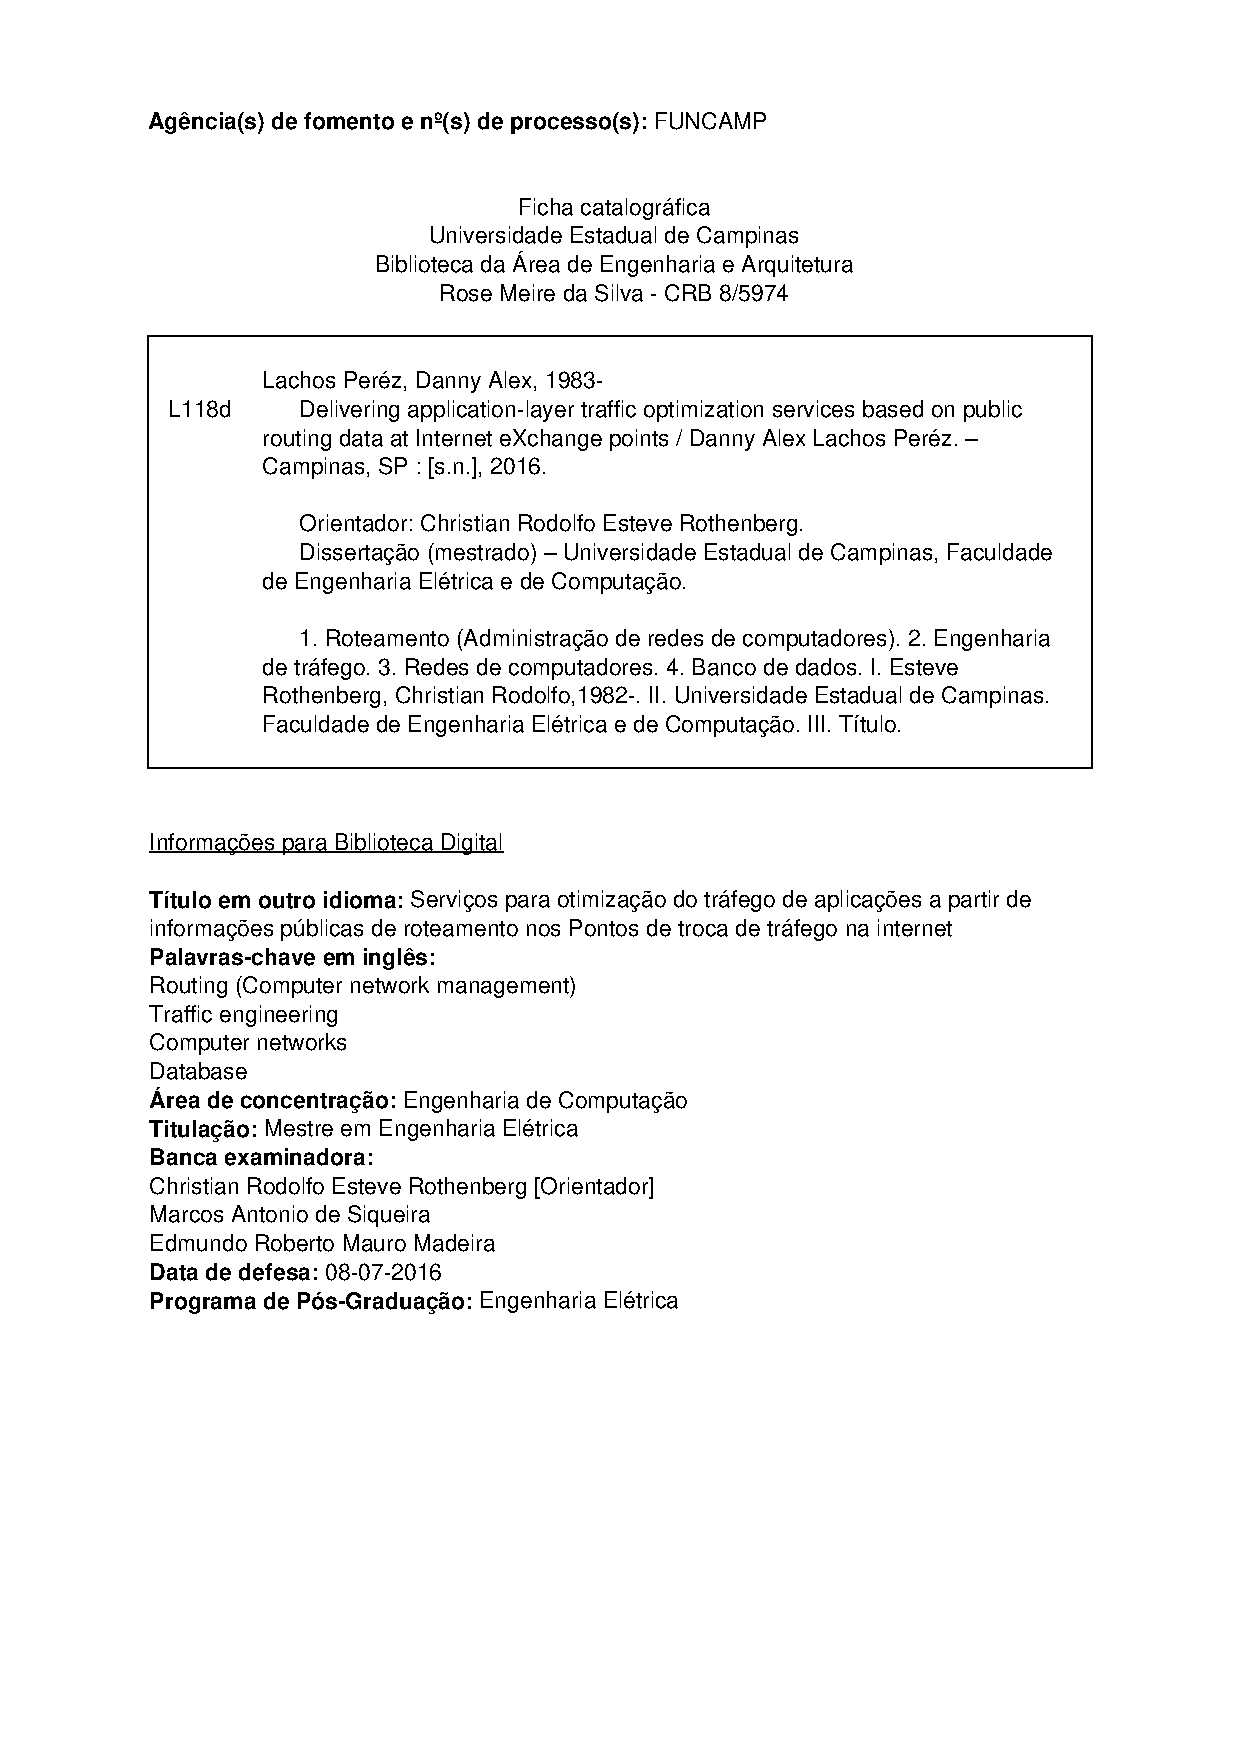
\includepdf[pages={1}]{docs/Ficha-Catalografica-Protocolo-86219375.pdf}
%
\includepdf[pages={1}]{figures/cat.jpg}
%\includepdf{ficha-catalografica.pdf}
\end{fichacatalografica}
% ---
\newpage
%\vspace*{\fill}
%\begin{center}
%    \textsc{Inclua aqui a folha de assinaturas.}
%\end{center}
\AtaDeDefesa

%\vspace*{\fill}
\newpage
% --- --- ---
%\includepdf[pagecommand={\thispagestyle{plain}}]{folha-assinaturas.pdf}	
%\cleardoublepage
% --- Dedicat\'{o}ria ---
\begin{dedicatoria}
\vspace*{\fill}
\centering
\noindent
\Dedicatoria
\vspace*{\fill}
\end{dedicatoria}


\begin{agradecimentos}
\Acknowledgements
\end{agradecimentos}

% ---
% --- Ep\'{\i}grafe  ---
\begin{epigrafe}
\vspace*{\fill}
\begin{flushright}
\begin{minipage}{9.9cm}
\Epigrafe
\end{minipage}
\end{flushright}
\begin{flushright}
\textit{\EpigrafeAuthor}
\end{flushright}
\end{epigrafe}

% ---
% --- RESUMOS (em portugu\^{e}s e ingl\^{e}s ---

\begin{resumo}
\Abstract
\newpage
\begin{otherlanguage*}{english}
\begin{center}{\ABNTEXchapterfont\huge Resumo}\end{center}
\Resumo
\end{otherlanguage*}
\end{resumo}


% --- inserir lista de ilustra\c{c}\~{o}es ---
\pdfbookmark[0]{\listfigurename}{lof}
\listoffigures*
\newpage
%\cleardoublepage
% ---

% --- inserir lista de tabelas ---
\pdfbookmark[0]{ \listtablename}{lot}
\listoftables*
\newpage
% ---
%\printglossary
%\cleardoublepage

\printglossary[type=\acronymtype]
\newpage
% --- inserir o sumario ---

\pdfbookmark[0]{\contentsname}{toc}
\tableofcontents*
\cleardoublepage
% ---

%\input{acronyms}
%\renewcommand{\nomname}{Acronyms and Abbreviations List}
%%\pdfbookmark[0]{\nomname}{las}
%\printnomenclature
\cleardoublepage
% ---
\pagenumbering{arabic}
\setcounter{page}{17}

% ---- ELEMENTOS TEXTUAIS ----
\textual

% ---- Introdu\c{c}\~{a}o ----
%%%%%%%%%%%%%%%%%%%%%%%%%%%%%%%%%%%%%%%%%%%%%%%%%%%%%%%%%%%%%%%%%%%%%%%%%%%%%%%%
\chapter{Introduction}\label{ch:introduction}
%%%%%%%%%%%%%%%%%%%%%%%%%%%%%%%%%%%%%%%%%%%%%%%%%%%%%%%%%%%%%%%%%%%%%%%%%%%%%%%

%4th-review
\section{Motivation}
 

The type of traffic used for performing evaluation matters; this is a fact. Studies show that realistic Ethernet traffic provides different and variable load characteristics on routers\cite{harpoon-validation}, even with the same average bandwidth consumption, showing that constant traffic is not sufficient for complete technology validation. This conclusion indicates that tests which employ traffic generators with constant rates are not enough for complete validation of new technologies. Bursty traffic can cause packet losses and buffer overflows, impacting on network performance and measurement accuracy\cite{burstiness-queue-lenght}. Small packets tend to degrade application performance\cite{comparative-trafficgen-tools}.  Furthermore, realistic traffic is essential on security research, such as for the evaluation of firewall middleboxes, studies on intrusion, and malicious workloads\cite{ditg-paper}. 

New networking scenarios such as \acrshort{SDN} and virtualized networks (\acrshort{NFV} and \acrshort{VNF}s) become harder to predict in terms of performance compared to hardware-based technologies, due to the multiple layers of software and platform parameters demanding validation in a broadening range of use cases~\cite{nfv-challenges}. Another critical question about the interaction between application-network has had the flow-oriented operation of SDN networks, in which each new flow arriving on an SDN switch demands further communication with the controller. Therefore the controller can be a bottleneck on the switches performance.  Also,  new types of traffic patterns introduced by \acrshort{IoT} and Machine-to-Machine (\acrshort{M2M}) communication\cite{machine2machine}  increase the complexity of the network traffic characterization, turning pre-defined models used by traffic generators obsolete. 

Furthermore, realistic traffic generators are essential security research, since the generation of realistic workloads is essential for evaluation of firewall middleboxes. It includes studies of intrusion, anomaly detection, and malicious workloads. By realistic, we refer to traffic that represents well the traffic features, such as protocols, payloads, and protocols, able to emulate benign and malicious workloads. 

Aiming to address these gaps, this dissertation introduces \acrshort{SIMITAR}, an auto-configurable network traffic generator. SIMITAR stands for \textit{SnIffing, ModellIng, and TrAffic geneRation}, which correspond to the main operation processes of the proposed framework.  SIMITAR has an application independent traffic model, that can represent a wide variety of scenarios. It also decouples the traffic modeling and packet-generation layer, using a factory design pattern, enabling its application on different scenarios, and technology update, via technology abstraction.  SIMITAR code and all scripts used in this paper are available at GitHub\cite{projeto-github} for validation, experiment reproducibility, and re-use purposes. 


\section{Related Work}


\begin{table*}[ht!]
    \centering
    \caption{Comparison of existing traffic generation tools.}
    \scalebox{0.80}{ 
    \begin{tabular}{ccccc}
        \hline
        \rowcolor[HTML]{9B9B9B} 
        \hline
        \textbf{Solution}     & \textbf{Auto-configurable} & \textbf{Realistic Traffic} & \textbf{Traffic Custumization} & \textbf{Extensibility} \\ \hline
        Harpoon     & yes              & yes               & yes                   & \textbf{no}   \\
        \rowcolor[HTML]{C0C0C0} 
        D-ITG                & \textbf{no}      & yes               & yes                   & \textbf{no}   \\
        Swing                & yes              & yes               & \textbf{no}           & \textbf{no}   \\
        \rowcolor[HTML]{C0C0C0} 
        Ostinato             & \textbf{no}      & \textbf{no}       & yes                   & yes           \\
        LegoTG               & \textbf{no}      & \textbf{no}       & yes                   & yes           \\
        \rowcolor[HTML]{C0C0C0} 
        sourcesOnOff          & \textbf{no}      & yes               & yes                   & \textbf{no}   \\
        Iperf                & \textbf{no}      & \textbf{no}       & yes                   & \textbf{no}   \\ 
        \rowcolor[HTML]{C0C0C0} 
        \textbf{SIMITAR}          & \textbf{yes}      & \textbf{yes}               & \textbf{yes}                   & \textbf{yes}   \\ \hline
    \end{tabular}
    }
    \label{tab:related-work}
\end{table*}



Traffic generators are tools to transfer or inject network packets in a controlled manner,  aiming not at the actual data transfer data but at the functional validation and performance benchmarking of devices under test (\acrshort{DUT}) for varying technologies or scenarios. The open-source community offers a vast variety of traffic generators. Since most have been built for specific goals,  each uses different methods for traffic generation, and offer control over different traffic features, such as throughput, packet-sizes, protocols, and so on\cite{ditg-paper}. 

Traffic generators can be classified into two main groups: replay engines\cite{sourcesonoff-paper} and model-based tools. Replay engines, such as TCPReplay and TCPivo\cite{tcpivo-paper}, work replicating in a given network interface a given packet capture file. These tools can generate realistic traffic but have their constraints. They are deterministic since will always reproduce the same traffic from the packet capture. Replay engines require storage of packet capture, what can be a problem for traffics of high bandwidth traffic. Also, they assume the user has access to packet captures appropriate for his testing purposes, which is not always true, due to a limited number of public sources. Model-based tools rely on software models to replicate one or more characteristics of the traffic. 

%Following the taxonomy presented by Botta et al.\cite{do-you-trust}:
%\begin{itemize}
%\item \textbf{Application-level traffic generators}: they try to emulate network applications simulating real workloads stochastically and(or) responsively. Eg.: Surge, D-ITG\footnote{D-ITG works mainly on packet-level but can emulate some applications}.
%\item \textbf{Flow-level traffic generators}: they can reproduce features of flows, such as flow duration, a diurnal behavior. Eg.: Harpoon\cite{harpoon-validation}.
%\item \textbf{Packet-level traffic generators}: most traffic generators available fall in this class. They aim to reproduce physical features such as inter-packet times, packet size, bandwidth and packets per second. Eg.: Iperf\cite{web-iperf}, Ostinato\cite{web-ostinato}, D-ITG\cite{ditg-paper}, sourcesOnOff\cite{sourcesonoff-paper}.
%\item \textbf{Multi-level traffic generators}: it proposes to take into account existing interaction among each layer of the network stack. Eg.: Swing\cite{swing-paper}.
%\end{itemize}

Model-based tools have their limitations as well. Traffic generators that emulate the applications,  are designed to represent only specific scenarios on computer networking, and are not enough to represent a large variety of scenarios. Many  traffic generator tools only offer constant-rate and Poisson models, which does not represent well the complexity of internet traffic\cite{selfsimilar-ethernet}. Other tools such as D-ITG offer dozens of parameters and models to be configured, but delegate to the user the task of creating, validate and script his traffic model. To the best of our knowledge, we found only two open-source auto-configurable tools: Swing and Harpoon.  However, none of them has an extensible architecture, which turns supporting modern and fast \acrshort{I/O} \acrshort{API}s (such as DPDK\cite{web-dpdk}) a hard task. Table~\ref{tab:related-work} present a summary of the above mentioned features for some relevant traffic generators: Swing\cite{swing-paper}, Harpoon\cite{harpoon-validation}, sourcesOnOff\cite{sourcesonoff-paper}, D-ITG\cite{ditg-paper}, Iperf\cite{web-iperf}, Ostinato\cite{web-ostinato} and LegoTG\cite{legotg-paper}.


\section{Objectives, Requirements, and Methodology}


Based on the provided context, we defined a set of targets for our research:


\begin{enumerate}

	\item \textbf{Survey}: Evaluate open-source Ethernet workload tools and address features each one has. We wanted to know the existing solutions, innovation points on the current state of affairs, and how can we some could be integrated and reused by our solution;
	
	\item \textbf{Background studies}: Study the characterization and mathematical modeling of Ethernet traffic, what are the best models and challenges. 
	
	\item \textbf{Definition of Realistic Traffic}: Define what realistic traffic generation is, and how to measure if any synthetic traffic is realistic or not. 
	
	\item \textbf{Design}: Create a general method for modeling and parameterization of Ethernet traffic;
	
	\item \textbf{Development}:  Create a self-configurable tool that observes and uses real network traffic, and reproduce its behavior characteristics, avoiding the storage of large \textit{pcap} files. 
	
\end{enumerate}

Towards the above-stated objectives, we  had identified a set of requirements of the envisioned traffic generation tool should meet:

\begin{itemize}

\item \textbf{Auto-configurable}: It must be able to extract data from real traffic and store in a database, and use it to parametrize its traffic model. It must be able to obtain data from real-time traffics and from \textit{pcap} files;

\item \textbf{Technology independent}: It must have a flow-based abstract model for traffic generation, not attached to any specific technology.

\item \textbf{Extensibility}: traffic modeling and generation must be decoupled. Ideally, it must be able to use as a traffic generator engine any library or traffic generator tool;

\item \textbf{Simple usage}: It must be easy to use. It has to take as input a Compact Trace Descriptor, just as a traffic replay engine (such as TCPreplay) would take a \textit{pcap} file;

\item \textbf{Human readable model}: it must produce a human-readable file as output that describes our traffic using our abstract model. We call this file a Compact Trace Descriptor (\acrshort{CDT});

\item \textbf{Traffic generation programmability}: It must have what we call traffic generation programmability. The compact trace descriptor must be simple and easy to read. That way, the user may want to create our custom traffic, in a platform agnostic way.

\item \textbf{Flow-oriented}: traffic modeling and generation must be flow-oriented. Each flow must be modeled and generated separately.

\end{itemize}


\begin{figure}[!ht]
    \centering
    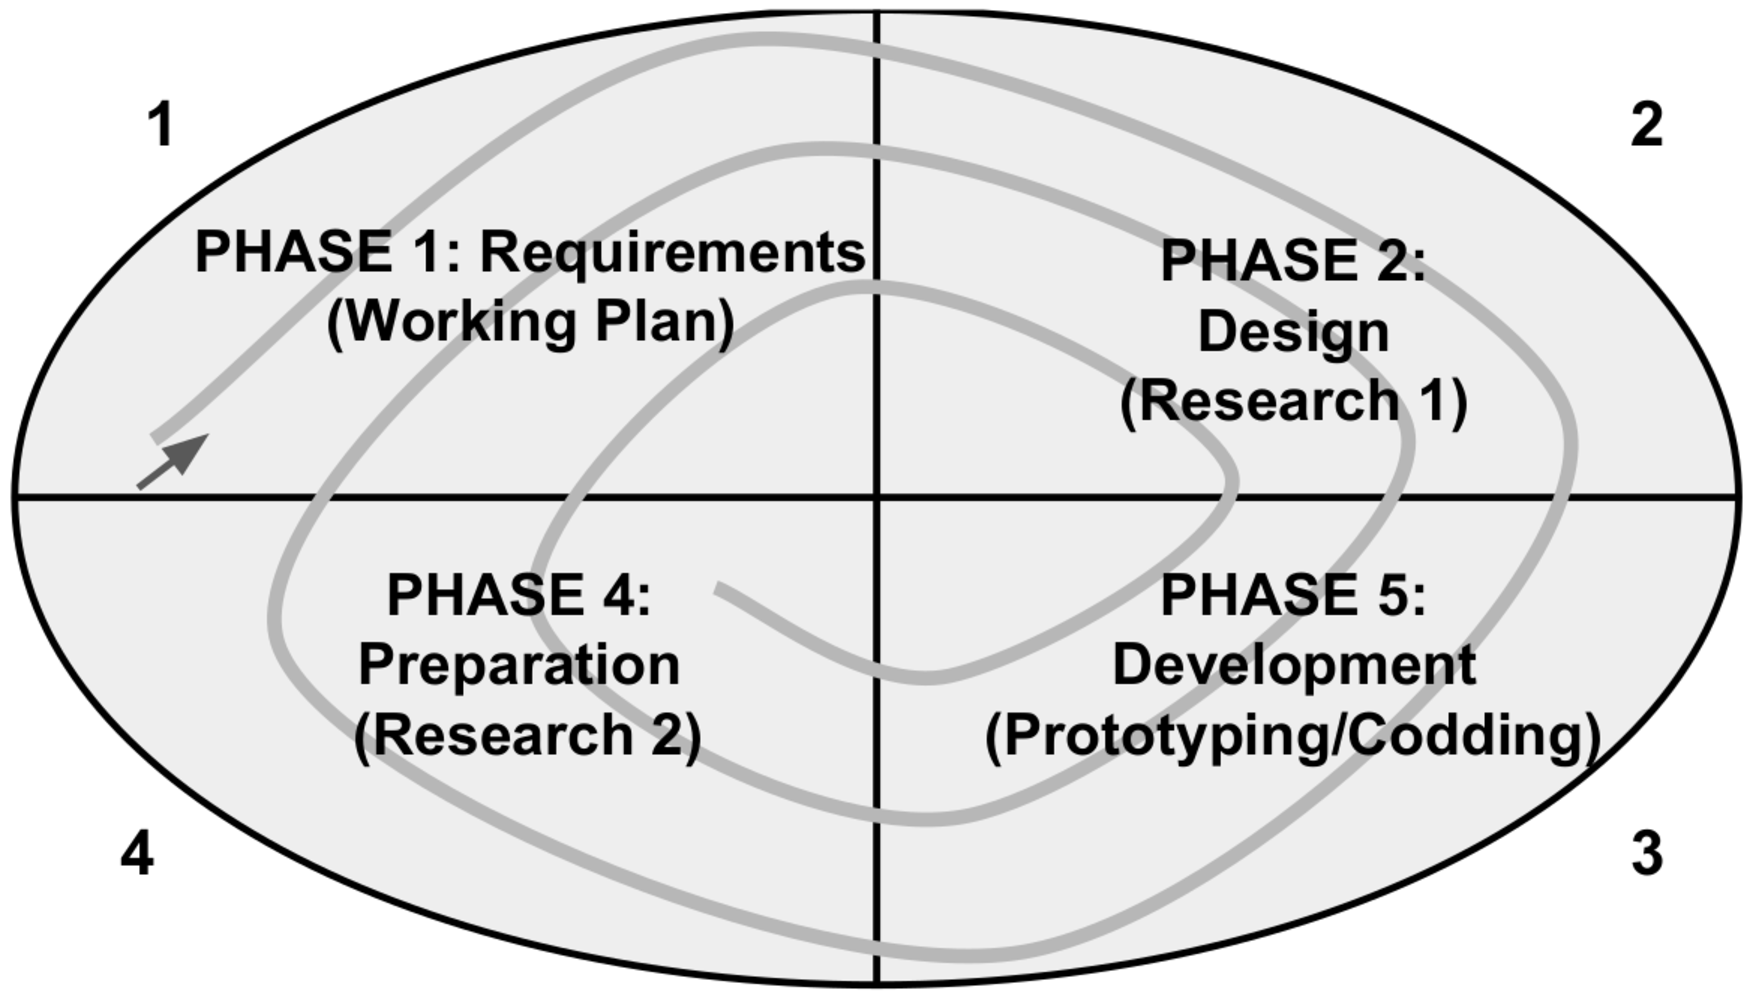
\includegraphics[scale=0.3]{figures/ch1/dev-cicle}
    \caption{Spiral research and development procedure}
    \label{fig:dev-cicle}
\end{figure}

We have adopted a spiral procedure of development, as suggested Sommerville on \textit{Software Engineering}\cite{sommerville}, but adapted to an academic research process. Figure~\ref{fig:dev-cicle} shows the model of development we had adopted. It had four main phases: 

\begin{enumerate}
    \item \textit{Requirements (working plan)};
    \item \textit{Design (research 1)};
    \item \textit{Development (prototyping/codding)};
    \item \textit{Preparation (research 2)}.
\end{enumerate}

On the \textbf{Requirements phase}, we create tasks,  formalized on \textit{Working Plans} documents.  These tasks should cover the whole process. On the \textbf{Design (research 1) phase}, where the focus of the research are related works. We research on literature to learn about topics defined by the task, to help we design our solutions. On this step, during the initial phases of the project,  we also conceived the architecture along with \acrshort{UML} diagrams\footnote{\textbf{Unified Modeling Language (UML)} is a modeling language designed to provide a standardized way of representing and design systems\cite{uml}.}. Some small changes are inevitable, but structural changes turn to be impractical on later phases. The next phase is the \textbf{Development phase}. It is the prototyping and coding phase.  The last is the \textbf{Preparation phase} when we evaluate the results achieved on the Development phase, and we go back to research again,  aiming to prepare the next \textit{Working Plan}.  On this phase, the focus of the research is on points of innovation.


\section{Outline}


In this introductory Chapter, we had presented an abstract of state of affairs, and the main goals of our research. \textit{\textbf{Chapter~\ref{ch:literature-review}}} presents a survey on open-source traffic generator tools, summarizing the benefits, and features supported by each one. The chapter offers a  review of topics on realistic traffic generation and defines important concepts on network traffic modeling; such as self-similarity and heavy-tailed distributions. Also, the chapter presents a survey on techniques for validating traffic generator tools 

\textit{\textbf{Chapter~\ref{ch:architecture}}} presents \textit{SIMITAR} traffic generator. We describe its low-level requirements and define an architecture and their algorithms.  We explain its operation and suggest some use cases. In \textit{\textbf{Chapter~\ref{ch:modeling-evaluation}}} we go deep on the modeling process we had developed for our traffic generator. We validate the effectiveness of Information Criteria \acrshort{AIC} and \acrshort{BIC} as a method selection of stochastic models for  Ethernet traffic.  We also discuss some other algorithms we developed such as \textit{calcOnOff} and the application protocol guesser. In \textit{\textbf{Chapter~\ref{ch:validation}}}, we define a set of metrics based on previous tests on validation of traffic generators found in the literature. Here, we focus on the packet, flow, and scaling metrics. We test our tool in an emulated SDN testbed with Mininet\cite{web-mininet}\footnote{\textbf{Mininet} is a network emulator. It can run a collection of  hosts, switches, routers and links over a single Linux kernel, using lightweight virtualization\cite{web-mininet-repo}.}, using OpenDayLight\cite{web-opendaylight} as a controller. 

\textit{\textbf{Chapter~\ref{ch:future-work}}}  highlights future actions to improve SIMITAR on realism and performance along with other future research avenues, including improving its computational performance, expand it to new APIs of traffic generation and calibration of its constants. Finally, we end the work presentation with a conclusion ( \textit{\textbf{Chapter~\ref{ch:conclusion}}}).

\textit{\textbf{Appendices}} \textit{\textbf{~\ref{ap:revision-probability}}}, \textit{\textbf{~\ref{ap:networks}}}, and \textit{\textbf{~\ref{ap:traffic-gen-survey}}} provide supplementary materials for Chapter\textit{\textbf{~\ref{ch:literature-review}}}: Review of Mathematical Concepts, Computer Networks, and Traffic Generators. Appendix\textit{\textbf{~\ref{ap:aditional-plots}}} provides charts in addition to those presented in Chapter~\ref{ch:modeling-evaluation}, and Appendix\textit{\textbf{~\ref{ap:uml}}} complements the presentation of the architecture discussed in Chapter~\ref{ch:architecture} by presenting SIMITAR  UML class-diagrams.
%%%%%%%%%%%%%%%%%%%%%%%%%%%%%%%%%%%%%%%%%%%%%%%%%%%%%%%%%%%%%%%%%%%%%%%%%%%%%%%%
\chapter{Literature Review}\label{ch:literature-review}
%%%%%%%%%%%%%%%%%%%%%%%%%%%%%%%%%%%%%%%%%%%%%%%%%%%%%%%%%%%%%%%%%%%%%%%%%%%%%%%%

%%%%%%%%%%%%%%%%%%%%%%%%%%%%%%%%%%%%%%%%%%%%%%%%%%%%%%%%%%%%%%%%%%%%%%%%%%%%%%%%
\section{A Brief Survey on Traffic Generators}\label{sec:traffic-gen}

A traffic generator is a tool capable of creating and injecting packets into a computer network in a controlled way to generate a synthetic traffic \cite{validate-trafficgen}.  There is a vast variety of traffic generators described on the literature \cite{validate-trafficgen} \cite{ditg-paper} and available in the open-source community\footnote{\href{http://www.icir.org/models/trafficgenerators.html}{http://www.icir.org/models/trafficgenerators.html}}. This is a consequence of an equally large amount of approaches for crafting synthetic traffic \cite{validate-trafficgen}.

The development of new network generators tightly related with to the current needs of network environment, applications sets, and purpose of use \cite{validate-trafficgen}. For example, if we want to evaluate the performance limits of equipment or new technology, you may want to execute stress tests, at specific constant rates. In this case, a maximum throughput traffic generator is more interesting\cite{validate-trafficgen}. On the other hand, to test how it performs on an actual network environment, you should search for a tool that produces a stochastically realist profile. Or, if you have a more specific usage case, you may search for a traffic generator that emulates an application scenario such as a client and a network server\cite{surge-paper}. 


Alongside with the variety of traffic generators, there are many APIs to create traffic. Some are low-level APIs which enables direct packet injection, such as \textit{libpcap}\cite{web-tcpdump}, \textit{libtins}\cite{web-libtins}, DPDK\cite{web-dpdk} and the GNU C socket library\cite{web-socket}. And there are high-level APIs, provided by traffic generator tools, such as D-ITG\cite{ditg-paper}, Ostinato\cite{web-ostinato} and MoonGen\cite{moongen-paper}. In this case, they enable an easy custom traffic generation and statistics. Also, there are implementations of hardware-based traffic generators using NetFPGAs\footnote{\href{http://netfpga.org/site/\#/}{http://netfpga.org/site/\#/}}.


There are many classifications of traffic generators\cite{sourcesonoff-paper}\cite{hybrid-traffic-gen}\cite{validate-trafficgen}\cite{do-you-trust}, and many have features that fall into more than one class. But classify them it is an efficient way to distinguish the difference between these tools. We will cite here two sorts of classification:

\begin{itemize}
	\item According to its abstraction level \cite{do-you-trust};
	%\item According to its purpose (engine replay, throughput, realism) \cite{validate-trafficgen}
	\item According to its implementation.
\end{itemize}

The most common classification is about its abstraction level\cite{do-you-trust}, and it divides the traffic generators in four groups: Application-level, flow-level, packet-level and multi-level traffic generators. We present a diagram illustrating its concept in figure ~\ref{fig:layers-workload-tools}.

%%%%%%%%%%%%%%%%%%%%%%%%%%%%%%%%%%%%%%%%%%%%%%%%%%%%%%%%%%%%%%%%%%%%%%%%%%%%%%%%
\subsection{According to its abstraction level}

\textbf{Application-level traffic generators}: they try to emulate the behavior of network applications, simulating real workloads stochastically or responsively \footnote{Responsiveness refers to the property of capacity of response over time of the workload tool. That means the behavior of the output may change according to what packets have arrived in the network interface}. As examples, we have Surge\cite{surge-paper}, which emulates the communication between clients and web servers.

\textbf{Flow-level traffic generators}: they can configure and reproduce flow characteristics\cite{do-you-trust}\cite{sourcesonoff-paper}, such as flow duration, start times distributions, and temporal (diurnal) traffic volumes\cite{do-you-trust}. Harpoon \cite{harpoon-paper} is able to extract these parameters from Cisco NetFlow data, collected from  routers.

\textbf{Packet-level traffic generators}: most common type of traffic generator. They can control packet-features like inter-departure times, packet size, throughput and packets per second\cite{validate-trafficgen}. \cite{validate-trafficgen} classify them as replay engines, maximum throughput generators, and model-based generators. Traffic Replay engines, such TCPreplay\cite{web-tcpreplay}, can read packet capture files (\textit{pcap} files), and inject copies on a network interface. Model-based generators, such D-ITG \cite{ditg-paper}, TG\cite{web-tg}, may have PS and IDT configured by the user. They can configure IDT  either by constant values (defining the packet rate or bandwidth) or by stochastic models. Maximum throughput engines like Ostinato and Seagull are tools that the main goal is to perform end-to-end stress testing. Are included in this category generators that can craft packets from the link layer, like Brute, KUTE, and pktgen.

\textbf{Multi-level traffic generators}: this is a more recent class of network traffic generator. They take into account existing interaction among each layer of the network stack, to create network traffic as close as possible to reality. Today, the most relevant tool is Swing \cite{swing-paper}. Swing take as input collected \textit{pcap} files. Botta at al. \cite{do-you-trust} argues that due its complexity, they are rarely used to conduct experimental researchers. Also, due its complexity, its performance is limited\cite{legotg-paper}. 

% On the other hand, D-ITG reached 9808 Mbps\cite{comparative-trafficgen-tools} in a link of 10 Gbps, but operating as a maximum throughput generator.


\begin{figure}[!ht]
	\centering
	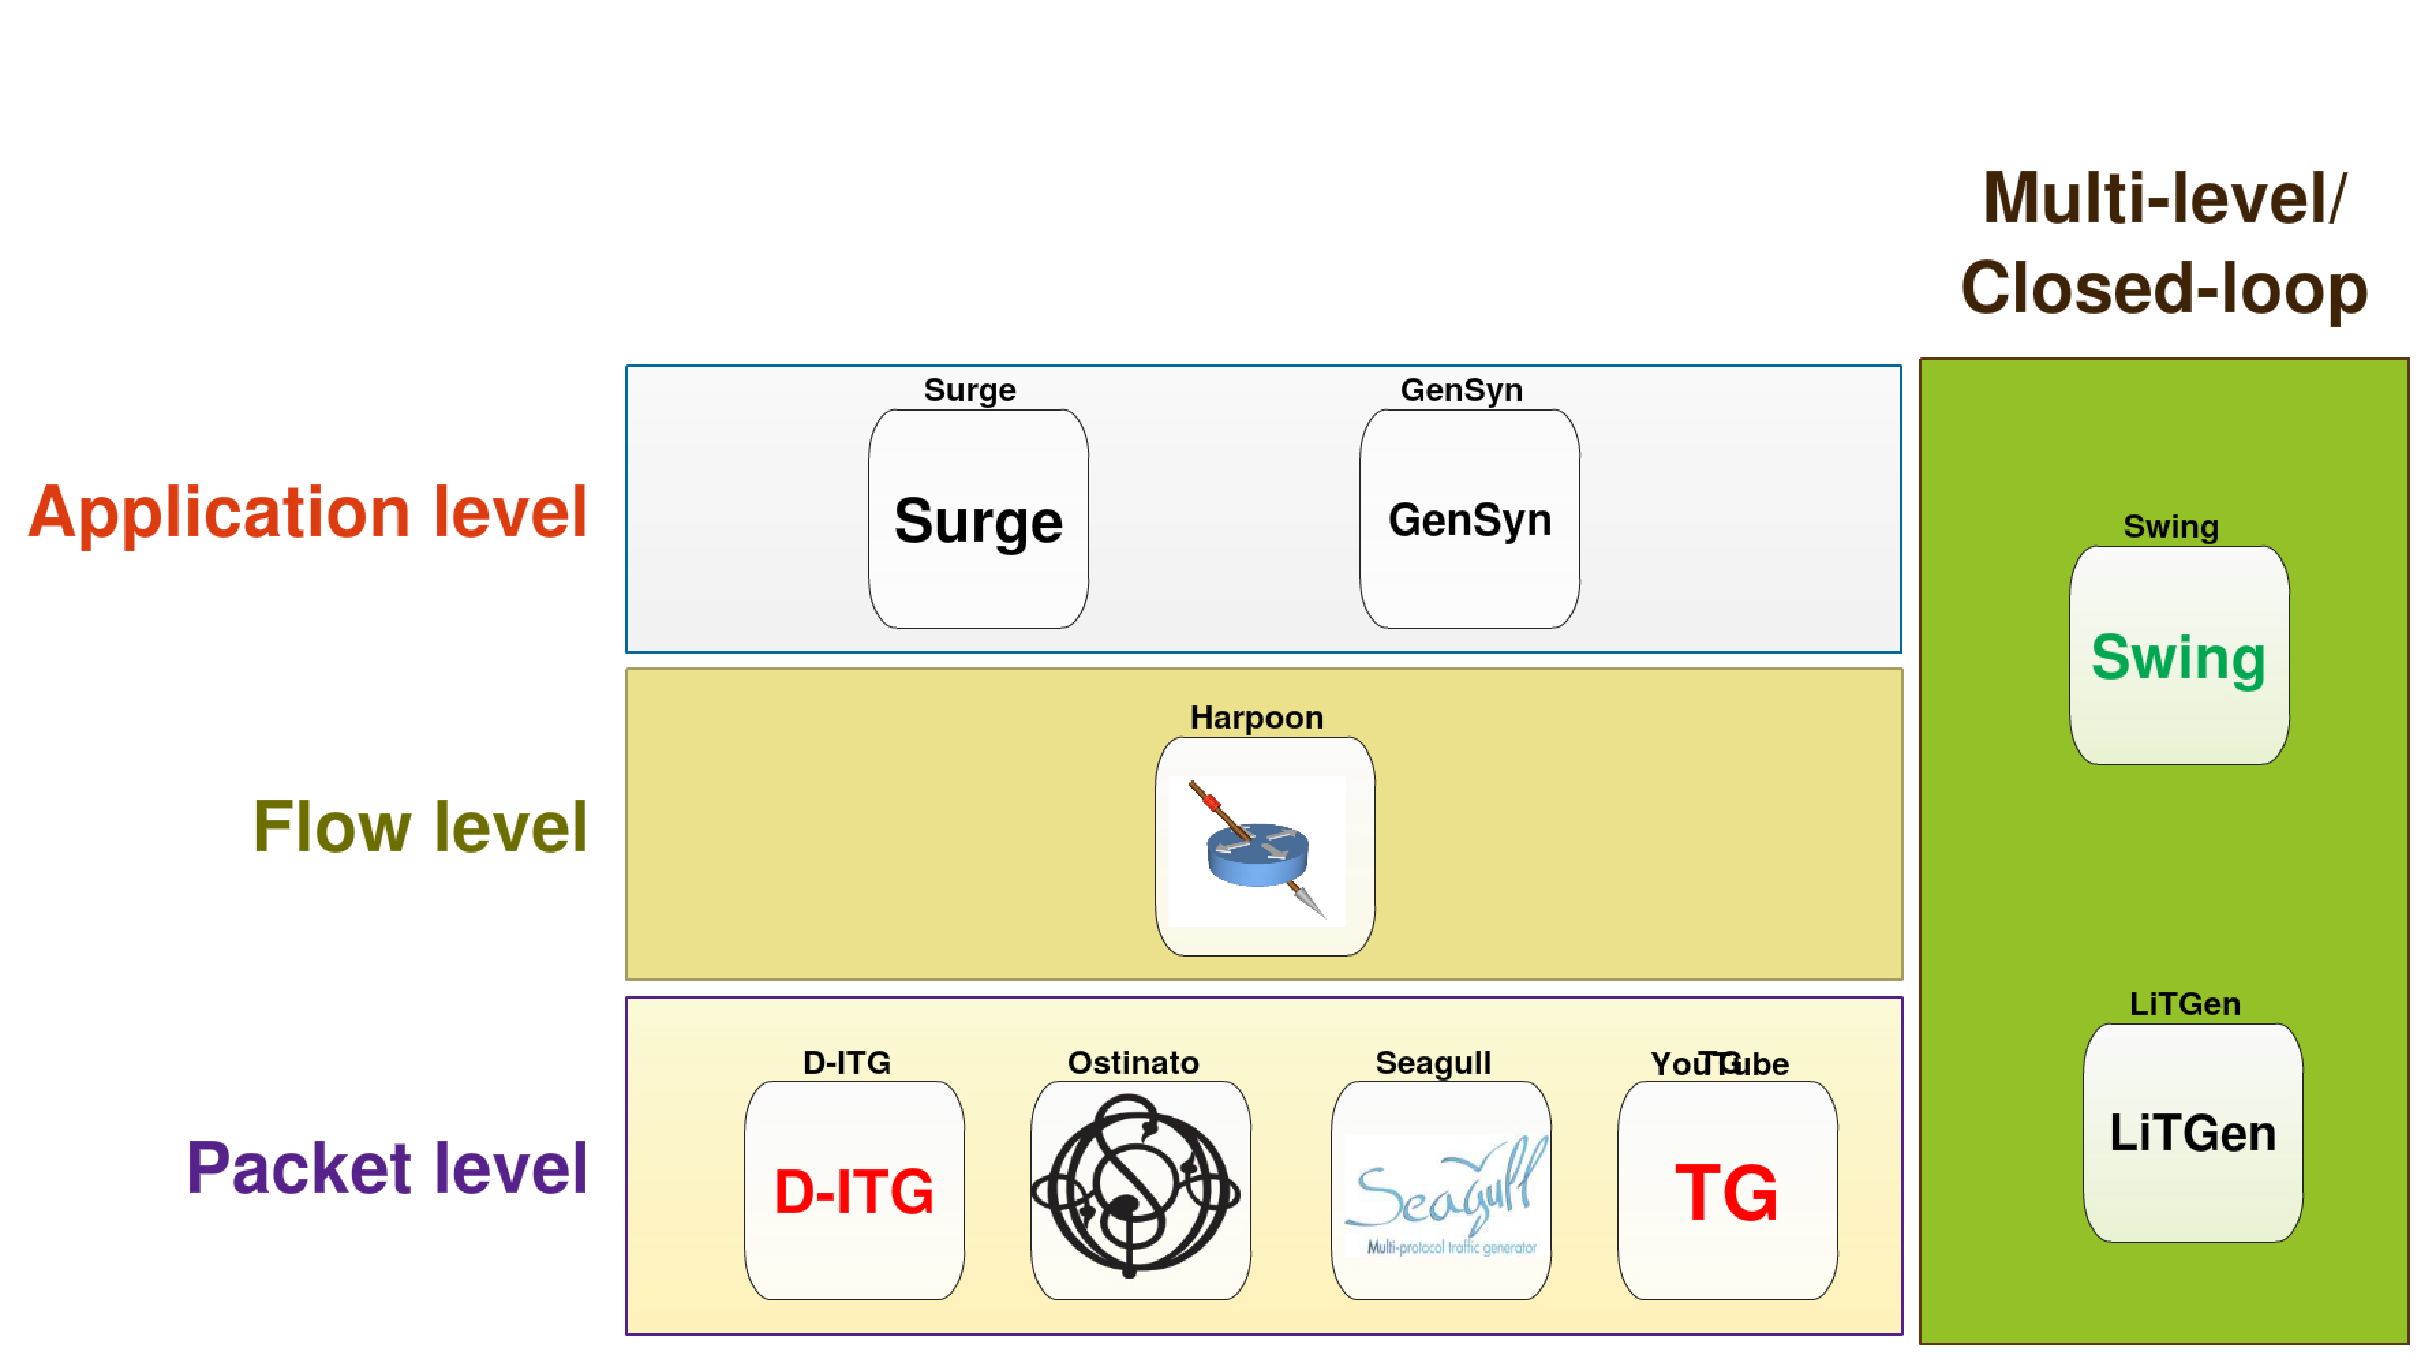
\includegraphics[scale=0.4]{figures/ch2/types-workload-tools}
	\caption{Diagram representing different traffic generators, according to its abstraction layer.}
	\label{fig:layers-workload-tools}
\end{figure}


%%%%%%%%%%%%%%%%%%%%%%%%%%%%%%%%%%%%%%%%%%%%%%%%%%%%%%%%%%%%%%%%%%%%%%%%%%%%%%%%
\subsection{According to its implementation}

\textbf{Software-only traffic generators}: Implementations of traffic generators utterly independent of its running hardware platform. This implementation comprehends most of traffic generator tolls.

\textbf{Software and hardware-dependent traffic generators}: Traffic generators implemented in software, but dependent on the underlying hardware. The most preeminent examples of this class are implemented over DPDK\cite{web-dpdk}. DPDK works directly on the NIC interface, avoiding overheads of the Operational System. As cited on its official website, this approach permits huge precision and speed in the timing of packets, since it can send and receive packets within less than 80 clock cycles.

\textbf{Hardware traffic generators}: This open-source traffic generators implementations are implemented in hardware description language (VHDL/Verilog), and work on NetFPGAs. Some examples of implementations are: PacketGenerator \cite{web-netfpgapacketgenerator}, Caliper \cite{web-caliper}, and OSNT Packet Generator \cite{web-osnt}.


%Tabela: revisao dos principais geradores de trafego
\renewcommand{\tabularxcolumn}[1]{>{\small}m{#1}}


\begin{table}[t!]
\caption{Review of features of some open-source traffic generators}
\begin{center}
\begin{footnotesize}
\begin{tabularx}{\linewidth}{
|>{\hsize=0.9\hsize\raggedright\arraybackslash}X	% 10% of 4\hsize 
|>{\hsize=1.16\hsize\centering\arraybackslash}X					% 30% of 4\hsize
>{\hsize=1.37\hsize\centering\arraybackslash}X					% 30% of 4\hsize
>{\hsize=1.16\hsize\centering\arraybackslash}X					% 30% of 4\hsize
>{\hsize=0.7\hsize\centering\arraybackslash}X					% 30% of 4\hsize
>{\hsize=0.7\hsize\centering\arraybackslash}X|					% 30% of 4\hsize
% sum=4.0\hsize for 4 columns
}
	\hline
	\textbf{Traffic Generator} & 
    \textbf{Operating System} & 
    \textbf{Protocols supported} & 
    \textbf{Stochastic distribution} & 
    \textbf{Interface} & 
    \textbf{Operation Level} \\
    
    \hline
    GenSyn	&
    Java virtual machine &
    TCP, UDP, IPv4 &
    (\textit{user model}, \textit{responsible}) &
    GUI &
    application-level \\
    			
    \hline
    Harpoon &
    FreeBSD 5.1-5.4, Linux 2.2-2.6, MacOS X 10.2-10.4, and Solaris 8-10 &
    TCP, UDP, IPv4, IPv6 &
    (\textit{flow-level model, based on a input trace})&
    CLI &
    flow-level\\    

    \hline
    D-ITG &
    Linux, Windows, Linux Familiar, Montavista, Snapgear &
    IPv4, IPv6, ICMP, TCP, UDP, DCCP, SCTP &
    Constant, uniform, exponential, pareto, cauchy, normal, poisson, gamma, on/off, \textit{pcap}&
    CLI, Script, API &
    packet-level \\
    
    \hline
    Ostinato &
    Linux, Windows, FreeBDS &
    Ethernet/802.3/LLC SNAP; VLAN (with QinQ); ARP, IPv4, IPv6, IP Tunnelling (6over4, 4over6, 4over4, 6over6);TCP, UDP, ICMPv4, ICMPv6, IGMP, MLD; HTTP, SIP, RTSP, NNTP etc... \textit{extensible}&
    constant &
    GUI, CLI, Script, API &
    packet-level\\
	 		
    \hline
    Seagull&
    Linux, Windows &
    IPv4, IPv6, UDP, TCP, SCTP, SSL/TLS and SS7/TCAP. \textit{extensible}&
    constant, poisson, \textit{responsible} &
    CLI, API &
    packet-level\\



    \hline
    PackETH &
    Linux, MacOS, Windows &
    ethernet II, ethernet 802.3, 802.1q, QinQ, ARP, IPv4, IPv6, UDP, TCP, ICMP, ICMPv6, IGMP &
    constant &
    CLI, GUI &
    packet-level \\ 

    \hline
    Iperf &
    Windows, Linux, Android, MacOS X, FreeBSD, OpenBSD, NetBSD, VxWorks, Solaris &
    IPv4, IPv4, UDP, TCP, SCTP &
    constant &
    CLI &
    packet-level \\ 
     
    \hline
\end{tabularx} 
\label{tab:trafficgen-list1}
\end{footnotesize}
\end{center}
\end{table} 
\clearpage

\begin{table}[t!]
\caption{Review of features of some open-source traffic generators}
\begin{center}
\begin{footnotesize}
\begin{tabularx}{\linewidth}{
|>{\hsize=0.9\hsize\raggedright\arraybackslash}X	% 10% of 4\hsize 
|>{\hsize=1.16\hsize\centering\arraybackslash}X					% 30% of 4\hsize
>{\hsize=1.37\hsize\centering\arraybackslash}X					% 30% of 4\hsize
>{\hsize=1.16\hsize\centering\arraybackslash}X					% 30% of 4\hsize
>{\hsize=0.7\hsize\centering\arraybackslash}X					% 30% of 4\hsize
>{\hsize=0.7\hsize\centering\arraybackslash}X|					% 30% of 4\hsize
% sum=4.0\hsize for 4 columns
}
	\hline
	\textbf{Traffic Generator} & 
    \textbf{Operating System} & 
    \textbf{Protocols supported} & 
    \textbf{Stochastic distribution} & 
    \textbf{Interface} & 
    \textbf{Operation Level} \\
   
    \hline
    Swing &
    Linux &
    IPv4, TCP, UDP, HTTP, NAPSTER, NNTP and SMTP &
    \textit{capture trace}  &
    CLI &
    closed-loop and multilevel \\     
   
    \hline
    BRUTE &
    Linux &
    IPv4, IPv6 &
    constant, poisson, trimoda &
    CLI &
    packet-level \\ 
    
         
    \hline
    SourcesOnOff &
    Linux &
    IPv4, TCP, UDP &
    on/off (Weibull, Pareto, Exponential and Gaussian) &
    CLI &
    packet-level \\      
     
     \hline
    TG &
    Linux, FreeBSD, Solaris SunOS &
    IPv4, TCP, UDP &
    Constant, uniform, exponential, on/off &
    CLI &
    packet-level \\ 
    
    \hline
    Mgen &
    Linux(Unix), Windows &
    IPv4, IPv6, UDP, TCP, SINK &
    Constant, exponential, on/off &
    CLI, Script &
    packet-level \\ 

     
     \hline
    KUTE &
    Linux 2.6 &
    UDP &
    constant &
    kernel module &
    packet-level \\ 
     
     \hline
    RUDE \& CRUDE &
    Linux, Solaris SunOS, and FreeBSD &
    IPv4, UDP &
    constant &
    CLI &
    packet-level\\      

     
     \hline
    NetSpec &
    Linux &
    IPv4,UDP, TCP &
    uniform, Normal, log-normal, exponential, Poisson, geometric, Pareto, gamma &
    Script &
    packet-level \\ 
     
     \hline
    Nping &
    Windows, Linux, Mac OS X &
    TCP, UDP, ICMP, IPv4, IPv6, ARP &
    constant &
    CLI &
    packet-level \\ 
     
     
     \hline
    TCPreplay &
    Linux &
    \textit{pcap} &
    constant, \textit{pcap} &
    CLI &
    packet-level (\textit{replay engine}) \\ 

     
     \hline
    TCPivo &
    Linux &
    \textit{pcap} &
    constant, \textit{pcap} &
    CLI &
    packet-level (\textit{replay engine}) \\ 

     \hline
     NetFPGA PacketGenerator &
     Linux &
     \textit{pcap} &
     constant &
     CLI &
     packet-level (\textit{hardware-based}) \\ 

 

    \hline
\end{tabularx} 
\label{tab:trafficgen-list2}
\end{footnotesize}
\end{center}
\end{table} 
\clearpage

\begin{table}[t!]
\caption{Review of features of some open-source traffic generators}
\begin{center}
\begin{footnotesize}
\begin{tabularx}{\linewidth}{
|>{\hsize=0.9\hsize\raggedright\arraybackslash}X	% 10% of 4\hsize 
|>{\hsize=1.16\hsize\centering\arraybackslash}X					% 30% of 4\hsize
>{\hsize=1.37\hsize\centering\arraybackslash}X					% 30% of 4\hsize
>{\hsize=1.16\hsize\centering\arraybackslash}X					% 30% of 4\hsize
>{\hsize=0.7\hsize\centering\arraybackslash}X					% 30% of 4\hsize
>{\hsize=0.7\hsize\centering\arraybackslash}X|					% 30% of 4\hsize
% sum=4.0\hsize for 4 columns
}
	\hline
	\textbf{Traffic Generator} & 
    \textbf{Operating System} & 
    \textbf{Protocols supported} & 
    \textbf{Stochastic distribution} & 
    \textbf{Interface} & 
    \textbf{Operation Level} \\
 
    \hline
    NetFPGA Caliper &
    Linux &
    \textit{pcap} &
    constant &
    CLI &
    packet-level (\textit{hardware-based}) \\  

    \hline
    NetFPGA OSNT &
    Linux &
    \textit{pcap} &
    constant &
    CLI &
    packet-level (\textit{hardware-based}) \\    
 
     \hline
     MoonGen &
     Linux &
     IPv4, IPv6, IPsec, ICMP, UDP, TCP &
     constant, poisson &
     Script API (Lua) &
     packet-level (\textit{hardware-dependent}) \\ 
     
    \hline
    Dpdk Pktgen &
    Linux &
    IPv4, IPv6, ARP, ICMP, TCP, UDP, \textit{pcap} &
    constant, \textit{pcap} &
    CLI, Script API (Lua) &
    packet-level (\textit{hardware-dependent})\\      
     
     \hline
     Dpdk NFPA &
     Linux &
     \textit{pcap} &
     constant, \textit{pcap} &
     CLI, Web &
     packet-level (\textit{hardware-dependent}) \\ 
     
     \hline
     LegoTG &
     Linux &
     \footnote{Depend on underlying tools used} &
     \footnote{Depend on underlying tools used}  &
     CLI, Script &
     packet-level \\  
 
     \hline
     LiTGen &
     \textit{missingInfo} &
     \textit{missingInfo} &
     \textit{wifi model} &
     \textit{missingInfo} &
     closed-loop and multilevel\\   
 
     \hline 
     gen\_send/ gen\_recv &
     Solaris, FreeBSD, AIX4.1, Linux &
     UDP &
     constant &
     CLI &
     packet-level \\

     \hline 
     mxtraf &
     Linux &
     TCP, UDP, IPv4 &
     constant &
     GUI, script &
     packet-level \\

     \hline 
     Jigs Traffic Generator (JTG) &
     Linux &
     TCP, UDP, IPv4, IPv6 &
     constant &
     CLI &
     packet-level \\

     \hline 
     SURGE &
     Linux &
     TCP, IPv4 &
     \textit{application model} &
     CLI &
     application-level\\


     \hline 
     Httperf  &
     Linux &
     TCP, IPv4 &
     \textit{application model} &
     CLI &
     aplication-level \\


     \hline 
     VoIP Traffic Generator &
     Linux &
     UDP, IPv4 &
     \textit{application model} &
     CLI &
     application-level \\

    \hline
\end{tabularx} 
\label{tab:trafficgen-list3}
\end{footnotesize}
\end{center}
\end{table} 
\clearpage




%%%%%%%%%%%%%%%%%%%%%%%%%%%%%%%%%%%%%%%%%%%%%%%%%%%%%%%%%%%%%%%%%%%%%%%%%%%%%%%%
\section{Network Traffic Modeling and Realistic Traffic Generation}\label{sec:modeling-traffic}


Along with the huge diversity of traffic generator tools, there are many traffic generation approaches, depending on the main purpose of the traffic generator. Maximum throughput traffic generators have in mind the idea of sending as much traffic through an interface as it can. But the generation of a realistic workload is a need for validation of many aspects of a new infrastructure. First, to generate a realist traffic, we need to define the complexity that our synthetic traffic must have, compared to real ones. Depending on our purpose, we may focus on one or more aspects of the traffic. For example, protocols, header customization, packet-level features (inter-departure, packet-size) and flow level features (number of flows and flow modeling).


As presented, there is a huge amount of open-source traffic generators available. Each of them with many different sets of features available. But, on the generation of realistic workload, the set of possibilities become much more restrict. On the other hand, there are many works on characterization, modeling, and simulation of different types of network workload \cite{ditg-paper}.


As stated by Botta et al.\cite{ditg-paper},  a synthetic network workload generation over real networks should be able to: (1) Capture real traces complexity over different scenarios; (2) Be able to custom change some specific properties generated traffic ; (3) Return measure indicators of performance experienced by the workload.


To generate realistic traffic workloads, two main approaches exist in the literature \cite{ditg-paper}. First, we have the trace-based generation, where replay engines generate the traffic. As examples, we have TCPreplay, TCPivo, and others. The other approach is an analytical model-based generation. In this case, the packet generation process depends on analytical and stochastic models. As examples of tools, we have Swing, D-ITG, TG, MGEN RUDE/CRUDE, Seagull, and many others.  These tools control traffic features using stochastic and analytical models and/or enable header customization. 


The advantage of the replay engine is its simplicity. There is no need for stochastic modeling of features. It just needs to know how to read the packet from a file, called \textit{pcap}, and replicate it on the internet interface. Most of the traffic features such as packet sizes, inter-departure, and packet headers will be realistic. But, its major issue is the storage space required to generate traffic without replication. In fact, depending on the throughput required, just some seconds of traffic replication will cost GB's of hard disk space. If it is necessary to generate traffic for a longer time, or good \textit{pcaps} traces are not available, analytical are necessary. 


Classical models for network traffic generation were the same used in telephone traffic, such as pure Poisson or Poisson-related, like Markov and Poisson-batch\cite{selfsimilar-ethernet}. They are able to describe the randomness of an Ethernet link but cannot capture the presence of "burstiness" in a long-term time scale, such as traffic "spikes" on long-range "ripples" \cite{selfsimilar-ethernet}. In fact, as we can see at \cite{selfsimilar-ethernet} the nature of the Ethernet traffic is self-similar. It has a fractal-like shape since characteristics seen in a small time scale should appear on a long-scale as well. This is most of the time referred as long-range dependence or degree of long-range dependence (LRD). One way to identify if a process is self-similar is checking its Hurst parameter, or Hurst exponent H, as a measure of the "burstiness" and LRD. In fact, a random process is self-similar and LRD  if 0.5 < H < 1 \cite{stochartic-selfsimilar}. Furthermore, some later studies advocate the use of more advanced multiscaling models (multifractal), addressed by investigations that state multifractal characteristics.

Another stochastic characteristic of the Ethernet traffic is high variability, or infinite variance. Processes with such characteristic are said to be heavy-tailed \cite{sourcesonoff-paper}. In practical terms, that means a sudden discontinuous change can always occur. Heavy tail means that a stochastic distribution is not exponentially bounded\cite{sourcesonoff-paper}. This means that a value far from the mean does not have a negligible probability of occurrence. We can express self-similar and heavy-tailed processes using heavy-tailed stochastic distributions, such as Pareto and Weibull. As a reference for these stochastic distributions, a list in the table ~\ref{tab:distributions-equations}. In the last column, we indicate if the distribution is or not heavy-tailed.

\begin{table}[t!]
\centering
\caption{Probability density function (PDF) and Cumulative distribution function (CDF) of some random variables, and if this stochastic distribution has or not self-similarity property. Some functions used to express these distributions are defined at the table ~\ref{tab:distributions-definitions} }
\label{tab:distributions-equations}
\scalebox{0.82}{ 
\begin{tabular}{lcccr}
Distribution & PDF Equation & CDF Equation & Parameters & Heavy-tailed\\ \hline
\\
\multirow{2}{*}{Poisson} & \multirow{2}{*}{$f[k] = \frac{e^{-\lambda}\lambda^k}{k!}$} & \multirow{2}{*}{$F[k] = \frac{\Gamma(\lfloor k + 1 \rfloor, \lambda)}{ \lfloor k \rfloor!}$} &  $\lambda > 0$  (mean, \\
 &  &  & variance) & no \\ 
\\ 
\multirow{2}{*}{Binomial} & \multirow{2}{*}{$f[k] = \binom{n}{k}p^{k}(1 - p)^{n - k} $} & \multirow{2}{*}{$F[k] = I_{1 - p}(n - k, 1 + k)$} &  $n > 0$ (trials)\\  &  &  &$p > 0$ (success)  & no \\ 
\\
\multirow{2}{*}{Normal} & \multirow{2}{*}{$f(t) =  \frac{1}{\sqrt[]{2\sigma^2}\pi}e^{\frac{(t - \mu)^2}{2\sigma^2}}$ } & \multirow{2}{*}{ $F(t) = \frac{1}{2}[ 1 + \text{erf}(\frac{t - \mu}{\sigma\sqrt[]{2}})]$ } &  $\mu$ (mean) \\ &  &  & $\sigma > 0$ (std.dev) & no \\ 
\\ 
\multirow{2}{*}{Exponential} & \multirow{2}{*}{ $f(t) = \begin{cases} \lambda e^{-\lambda t} ;& t \geq 0 \\ 0;& t < 0 \end{cases} $  }   & \multirow{2}{*}{ $F(t) = 1 - e^{-\lambda t} $ } & \\ &  &  & $\lambda > 0$ (rate)  & no \\ 
\\
\multirow{2}{*}{Pareto} & \multirow{2}{*}{$f(t) = \begin{cases} \frac{\alpha t_{m}^\alpha}{t^{\alpha + 1}} ;& t \geq t_{m} \\ 0;& t < t_{m} \end{cases} $ } & \multirow{2}{*}{$F(t) = \begin{cases} 1 - (\frac{t_{m}}{t})^\alpha ;& t \geq t_{m} \\ 0;& t < t_{m}\end{cases} $} &  $\alpha > 0$ (shape)  \\ & &  &  $t_{m} > 0$ (scale)   & yes \\ 
\\ 
\multirow{2}{*}{Cauchy} & \multirow{2}{*}{ $f(t) = \frac{1}{\pi \gamma}[\frac{\gamma^2}{(t - t_{0})^{2} + \gamma^{2}}]$ } & \multirow{2}{*}{ $F(t) = \frac{1}{\pi}\arctan( \frac{t - t_{0}}{\gamma} ) + \frac{1}{2}  $ } &  $\gamma > 0$ (scale) \\ &  &   & $t_{0} > 0$ (location) & yes \\  
\\
\multirow{2}{*}{Weibull} & \multirow{2}{*}{ $f(t) = \begin{cases} \frac{\alpha}{\beta^\alpha}t^{\alpha - 1}e^{(t/\beta)^{\alpha}}; & t \geq 0 \\ 0; & t < 0 \end{cases}$  } & \multirow{2}{*}{ $F(t) = \begin{cases} 1 - e^{-(t/\beta)^{\alpha}}; & t \geq 0 \\ 0 ; & t < 0  \end{cases}$ } & $\alpha  > 0 $ (shape) \\ &  &  & $\beta > 0$ (scale)  & yes \\
\\
\multirow{2}{*}{Gamma} & \multirow{2}{*}{ $ f(t) = \frac{\beta^{\alpha}}{\Gamma(\alpha)}t^{\alpha - 1}e^{-\beta t}  $ } & \multirow{2}{*}{$ F(t) = 1 - \frac{1}{\Gamma(\alpha)}\Gamma(\alpha, \beta x) $} & $\alpha > 0$ (shape) \\ &  &  & $\beta > 0$ (rate) & no \\
\\ 
%\multirow{2}{*}{Student's t} & \multirow{2}{*}{} & \multirow{2}{*}{} &  \\ &  &  & & \\ 
%\\
\multirow{2}{*}{Beta} & \multirow{2}{*}{ $ f(t) = \frac{x^{\alpha - 1}(1 - x)^{\beta - 1}}{B(\alpha, \beta)} $ } & \multirow{2}{*}{ $ F(t) = I_{x}(\alpha, \beta) $ } &  $\alpha > 0$ (shape) \\ &  &  & $\beta > 0$ (shape) & no \\ 
\\ 
\multirow{2}{*}{Log-normal} & \multirow{2}{*}{ $ f(t) = \frac{1}{t \sigma \sqrt[]{2 \pi}}e^{- \frac{(\ln(x) - \mu)^{2}}{2 \sigma^{2}}} $ } & \multirow{2}{*}{ $ F(t) = \frac{1}{2} + \frac{1}{2}\text{erf}[\frac{\ln(x) - \mu}{\sqrt[]{2} \sigma}] $ } & $\mu$ (location)\\
 &  &  & $ \sigma > 0 $ (shape) & yes \\ 
\\
\multirow{2}{*}{Chi-squared} & \multirow{2}{*}{ $ f(t) = \frac{1}{2^{\frac{k}{2}}\Gamma(\frac{k}{2}) }t^{\frac{k}{2} - 1}e^{-\frac{t}{2}} $ } & \multirow{2}{*}{ $ F(t) = \frac{1}{\Gamma(\frac{k}{2})}\gamma(\frac{k}{2}, \frac{x}{2}) $ } &  \\
 &  &  & $ k \in \mathbb{N}_{>0} $ &  no\\ 
\\
 
\hline
\end{tabular} 
} %scalebox
\end{table}

\begin{table}[t!]
\centering
\caption{Definitions of some functions used by PDFs and CDFs}
\label{tab:distributions-definitions}
\begin{tabular}{ll}
\hline
Function                             & Definition \\ 
\hline
\\
Regularized Incomplete beta function & $ I_{x}(a, b) = \frac{B(x| a, b)}{B(a, b)} $           \\
\\
Incomplete beta function             & $ B(x| a, b) = \int_{0}^{x} t^{a - 1} (1 - t)^{(b - 1)} \text{d}t $           \\
\\
Beta function                        & $ B(x| a, b) = \int_{0}^{1} t^{a - 1} (1 - t)^{(b - 1)} \text{d}t $           \\
\\
Error function                       & $ \text{erf}(x) = \frac{1}{\sqrt[]{\pi}}\int_{x}^{-x} e^{-t^{2}} \text{d}t $           \\ 
\\
Lower incomplete Gamma function      & $ \gamma(s, x) = x^{s}\Gamma(s)e^{-x}\sum_{k = 0}^{\infty}\frac{x^{k}}{\Gamma(s+k+1)} $  \\
\\
\hline
\end{tabular}
\end{table}


We call these concepts of High variability and Self-similarity Noah and Joseph Effects \cite{selfsimilar-highvariability}. We can see at\cite{selfsimilar-highvariability} that a superposition of many ON/OFF sources (or packet trains) using ON and OFF that obey the Noah Effect (heavy-tailed probabilistic functions), also obey the Joseph effect. That means, it is self-similar and we can use to describe an Ethernet traffic. As we can see, some works on the literature on synthetic traffic uses this principle, like sourcesOnOff\cite{sourcesonoff-paper}, or have to support models like D-ITG\cite{ditg-paper}.


An accurate replication of a workload should be able to control packet headers such as QoS fields, protocols, ports, addresses, and so on. Traffic generators provide support for these features, more frequently in a limitted way. Most offer support just common protocols, such as TCP, UDP, and IPv4. On the other hands, there are some which provide a huge variety of support and control over packet headers like PackETH\cite{web-packeth} and D-ITG. Other tools are even able to enable you to extend this feature and develop support to new protocols. For example, Ostinato and Seagull permit you to define your own customized protocol.

%revisão da sessão 0.1 até aqui

Another relevant feature is the packet size distribution. As we can see in many works, the packet size of a trace may result in a huge impact in a trace throughput \cite{stochartic-selfsimilar}\cite{performance-trafficgen}, since small packets cause a larger overhead on packet processing. To exemplify, in the table~\ref{tab:packet-size-impact} we survey results from two different works \cite{comparative-trafficgen-tools} \cite{performance-trafficgen} about throughput impact of packet sizes. On packet size distribution characterization, we can find many works in the literature. For example, \cite{packet-distribution-model} analyses many packet sizes distributions of many packet traces, in many environments. Some general results are that \textbf{\textit{90\%}} of UDP packets are smaller than 500 bytes, and most packets transmitted using TCP have \textbf{\textit{40 bytes}} (acknowledgment) and \textbf{\textit{1500}} bytes (Maximum Transmission Unit, MTU) \cite{packet-distribution-model}. For UDP traffic, we have similar results, since mostly they are bimodal as well \cite{udp-flows-model}. Ostrowsky et al.\cite{udp-flows-model} found that, on UDP traces the modes of two regions are \textbf{\textit{120}} and \textbf{\textit{1350}} bytes, with a \textbf{\textit{cut-off}} value of \textbf{\textit{750 bytes}}. They also find that roughly UDP packets constitute \textbf{\textit{20\%}} of the total number of packets on captures. 


\begin{table}[t!]
\centering
\caption{Two different studies evaluating the impact of packet size on the throughput. Both compare many available open-source tools on different testbeds. In all cases, small packet sizes penalize the throughput. Bigger packet sizes achieve a higher throughput.}
\label{tab:packet-size-impact}
\scalebox{0.9}{
\begin{tabular}{|l|c|c|c|}
\hline
 & \multicolumn{3}{c|}{Traffic Generators} \\ \cline{2-4} 
\multicolumn{1}{|c|}{Article and setup} &  & \multicolumn{1}{c|}{Maximum bit-rate} & \multicolumn{1}{c|}{Maximum bit-rate} \\
 & \multicolumn{1}{c|}{Toll} & \multicolumn{1}{c|}{\begin{tabular}[c]{@{}c@{}}at small packet \\ sizes\end{tabular}} & \multicolumn{1}{c|}{\begin{tabular}[c]{@{}c@{}}at big packet \\ sizes\end{tabular}} \\ \hline
\textit{\begin{tabular}[c]{@{}l@{}}Comparative study of various \\ Traffic Generator Tools \cite{comparative-trafficgen-tools} ;\end{tabular}} & PackETH & 150 @(64 bytes) & 1745 @(1408 bytes) \\ \cline{2-4} 
\begin{tabular}[c]{@{}l@{}}setup: Linux (Centos 6.2, \\ Kernel version 2.6.32),\end{tabular} & Ostinato & 135 @(64 bytes) & 2850 @(1408 bytes) \\ \cline{2-4} 
\begin{tabular}[c]{@{}l@{}}Inter(R) Xeon(R) CPU with 2.96GHz,\\  RAM of 64GB , NIC Mellanox\end{tabular} & D-ITG & 62 @(64 bytes) & 1950 @(1408 bytes), \\
\begin{tabular}[c]{@{}l@{}}Technologies MT25418 {[}ConnectXVPI \\ PCIe 2.0 2.5GT/s - IB DDR{]}\end{tabular} &  &  & \begin{tabular}[c]{@{}l@{}}9808 @(1460 bytes, \\ 12 threads)\end{tabular} \\ \cline{2-4} 
10 Bbps. Protocol: TCP & Iperf & * & \begin{tabular}[c]{@{}l@{}}8450 @(1460 bytes, \\ 12 threads)\end{tabular} \\ \hline
\textit{\begin{tabular}[c]{@{}l@{}}Performance Monitoring of Various \\ Network Traffic Generators \cite{performance-trafficgen};\end{tabular}} & Iperf & 46.0 @(128 bytes) & 93.1 @(1408 bytes) \\ \cline{2-4} 
\begin{tabular}[c]{@{}l@{}}Inter(R) Pentium 4(R), CPU \\ with 3.0GHz, RAM 1GB,\end{tabular} & Netperf & 46.0 @(128 bytes) & 89.9 @(1408 bytes) \\ \cline{2-4} 
\begin{tabular}[c]{@{}l@{}}NIC Intel Pro/100 Adapter \\ (100Mbps),\end{tabular} & D-ITG & 38.1 @(128 bytes) & 83.1 @(1408 bytes) \\ \cline{2-4} 
\begin{tabular}[c]{@{}l@{}}Hard Drivers Seagate Barracuda \\ 7200 series with 20BG. \\ Protocol:TCP\end{tabular} & IP Traffic & 61.0 @(128 bytes) & 76.7 @(1408 bytes) \\ \hline
\end{tabular}
}
\end{table}


As could be expected, router capture traces, are mostly bimodal, since most of the traffic in backbones is TCP. But, the size of the each mode may change depending on the application. For example, a www usage tends to have a mode close to the MTU higher if compared to an FTP capture. So, for packet workload generation, these results suggest the importance of controlling the packet size behavior for each flow\cite{packet-distribution-model}.

On flow level traffic generation, some packet-level traffic generators permit the control of flow generation, mostly by manually controlling headers parameters through an API or via scripting. In terms of automatic flow configuration, an example is Harpoon\cite{harpoon-paper} which can to automatic configure its flows, using as input NetFlow Cisco traffic traces to automatically setting parameters. Harpoon deals with flow modeling in three different levels: file level, session level, and user level, not dealing with packet level at all.  In the file level, Harpoon model two parameters:  the size of files being transferred, and the time interval between consecutive file requests, called inter-file request time. The middle level is the session level, that consist of sequences files transfer between two distinct IP addresses. The session level has three components: the IP spatial distribution, the second is the inter-session start times and the third is the session duration. The last level is the user level. In Harpoon, "users" are divided on "TCP" and "UDP" users. Which conduct consecutive session using these protocols. This level has two components: the user ON time, and the number of active users. By modeling the number of users, harpoon can reproduce temporal(diurnal) traffic volumes, which is an interesting feature, once it is common on Internet traffic. 

A feature that may be highly desirable for realistic traffic generation is  operating in closed-loop like Swing\cite{swing-paper}. This means when the changes its behavior at run time according to the observation made in real-time, with involves modification of the traffic to be generated \cite{ditg-paper}. These modifications involve changes on parameters of statistical distributions of inter-departure time (IDT) and packet size (PS).

Closed-loop multi-layer and application layer traffic generators also models application and user behavior, like the number of request/response exchanges per connection, response sizes, request sizes, user think time between connections, the number of RREs, RREs think time, etc \cite{swing-paper}.

Finally, on newly arrived internet scenarios, due its increasing complexity of networks and the rise of many new technologies, such as SDN\cite{sdn-survey} and NFV\cite{nfv-challenges}; which include the replacement of old and reliable technologies by new and not as strongly validated ones. In this sense that a point to point validation is not enough anymore, an arriving requirement is the distributed workload generator, which includes a logically centralized module such as a controller\cite{ditg-paper}, or an orchestrator\cite{legotg-paper}, able to control and synchronize and deploy workloads of many different hots. As examples, D-ITG API gives this possibility via daemons, and LegoTG\cite{legotg-paper} Framework implements a complete and easily extensible orchestrator. Due new scenarios where virtualization network functions and hardware is overcoming hardware, a logically centralized control and orchestration of synthetic workloads is a feature that easy the work\cite{legotg-paper}.


%%%%%%%%%%%%%%%%%%%%%%%%%%%%%%%%%%%%%%%%%%%%%%%%%%%%%%%%%%%%%%%%%%%%%%%%%%%%%%%%
\section{Validation of Traffic Generator Tools}~\label{sec:validation-traffic-gen}

After the implementation of a traffic generator, it has to be validated. Thus, we need a set of proof of concepts to evaluate if it reached its purposes or not. 
There are many validation techniques researchers have proposed over time, according to the traffic generator intended behavior.  Magyesi and Szabó\cite{validate-trafficgen} presented on their work a survey of these techniques, grouped by type of metric. The authors classify them into four categories: packet based metrics, flow-based metrics, scaling characteristics and QoS/QoE related metrics. As suggested by other works\cite{swing-paper}, we state here that synthetic traffic can be considered realistic, metrics of these four classes are close to measured in a real scenario. Here we present a short review of each of these validation techniques. 


%%%%%%%%%%%%%%%%%%%%%%%%%%%%%%%%%%%%%%%%%%%%%%%%%%%%%%%%%%%%%%%%%%%%%%%%%%%%%%%%
\subsection{Packet Based Metrics}

Packet based are the most simple and more used metrics in the validation of traffic generators \cite{validate-trafficgen}. The most relevant packet based metrics are throughput\cite{do-you-trust}\cite{comparative-trafficgen-tools}\cite{performance-trafficgen}\cite{moongen-paper} (bytes and packets), packet size distribution\cite{packet-distribution-model} and inter packet time distribution (inter-arrival and inter-departure) \cite{sourcesonoff-paper} \cite{ditg-paper}.       


%%%%%%%%%%%%%%%%%%%%%%%%%%%%%%%%%%%%%%%%%%%%%%%%%%%%%%%%%%%%%%%%%%%%%%%%%%%%%%%%
\subsection{Flow Based Metrics}

Flow-based metrics are becoming more critical since newer network elements, like SDN devices, are able of executing flow-based operations\cite{validate-trafficgen}\cite{sdn-survey}. Magyesi and Szabó\cite{validate-trafficgen} consider the essential flow metrics the flow size distribution and the flow volume. The flow volume stands for the number of flows of traffic. The flow size distribution is a measure of the length of time and in size of data of each flow in network traffic. The flow volume is proportional to the number of flow instances that a flow-based device should run simultaneously. And the flow sizes defines how much time each of these instances will  run.


%%%%%%%%%%%%%%%%%%%%%%%%%%%%%%%%%%%%%%%%%%%%%%%%%%%%%%%%%%%%%%%%%%%%%%%%%%%%%%%%
\subsection{Fractal and Scaling Characteristics}

Second order characteristics such as burstiness and long-range dependence are responsible for the complex nature of the internet traffic\cite{validate-trafficgen}. Due its non-stationary nature, traditional methods fail on extract useful information\cite{validate-trafficgen}. The first analysis made in that way focused on the estimation of the Hurst exponent\cite{selfsimilar-ethernet}. They demonstrated the self-similar nature of the Ethernet traffic. As explained before, self-similar traffic should a Hust exponent $H$, such as $ 0.5 < H < 1$. Over the years, wavelet-based analysis has become an efficient way of reveal correlations, bursts and scaling nature of the ethernet traffic\cite{validate-trafficgen}. Many works found on the literature have used wavelet-based analysis \cite{swing-paper}\cite{non-intrusive-wavelet}\cite{wavelet-analysis-long-range}. 

Huang et al. \cite{non-intrusive-wavelet} and Abry and Veitch \cite{wavelet-analysis-long-range} offers an extensible explanation of wavelet-based scaling analysis (WSA) or wavelet multi-resolution energy analysis (WMA). Here, is presented a summary of the primary information offered by these two works, which you should refer to, for further details. 

First, consider a time series $X_{0,k}$ for $k = 0, 1, ... 2^n$:

\begin{equation}
\{X_{0,k}\} = \{ X_{0,0}, X_{0,1}, ... ,X_{0,2^{n}} \}
\end{equation} 

Supose then that we coaser $X_{0}$ in another time-serie $X_{1}$ with half of the original resolution, but using  $ \sqrt[]{2} $  as normalization factor:

\begin{equation}
X_{1,k} = \frac{1}{\sqrt{2}}(X_{0,2k} + X_{0,2k+1})
\end{equation}

If we take the differences, instead of the averages, evaluate the so-called \textit{details}. 

\begin{equation}
d_{1,k} = \frac{1}{\sqrt{2}}(X_{0,2k} - X_{0,2k+1})
\end{equation}

We can continue repeating this process, writing more coarse time series $X_{2}$ from $X_{1}$, until we reach $X_{n}$. Therefore, we will get a collection of \textit{details}:

\begin{equation}
\{d_{j,k}\} = \{ d_{1,0}, d_{1,1}, ..., d_{1,2^{n/2}}, ..., d_{n, 0} \}
\end{equation} 


This collection of details ${d_{j,k}}$ are called Discrete Haar Wavelet Transform. Using the \textit{details} we can calculate the energy function $E_{j}$, for each scale $j$, using:

\begin{equation}
E_{j} = \frac{1}{N_{j}} \sum_{k = 0}^{N_{j} - 1} |d_{j,k}|^{2}; \qquad j = 1, 2, ..., n
\end{equation} 
\\ 
were $N_{j}$ is the number of coefficients at scale $j$. If we plot $\log(E_{j})$ as a function o the scale $j$, we will obtain an wavelet multiresolution energy plot. 

On energy wavelet multiresolution energy plots, we can capture three different main behavior, according to the scale.  On \textbf{periodic time series}, the Energy values will be small. In fact, on perfectly periodic scales $j$, the values of the energy function $E_{j}$ will be zero. So periodicity will be sensed if the value of the energy function decrease. Perfect \textbf{white noise time series} will maintain the same value of the energy function. So an approximately constant values for the energy function $E_{j}$ indicates white noise behavior (which can be represented by a Poisson process\cite{poisson-white-noise}). On \textbf{self-similar time series}, the energy function plot $\log(E_{j})$ will grow approximately linearly with the scale $j$.  This explains why it has become a standard for realistic traffic generation analysis. In a single plot, we can easily identifiy periodicities, and self-similar and Poisson process characteristics, just seeing if it decays, grow, or remain constant.

Some recent works suggest the use of multi-fractal models, instead of the self-similar models (also called monofractal)\cite{validate-trafficgen}\cite{udp-flows-model}. Since there is a lack of multiscaling analysis on the literature on validation of traffic generators, this type of analysis will stay for future works. 

\begin{figure*}[ht!]
	\centering
	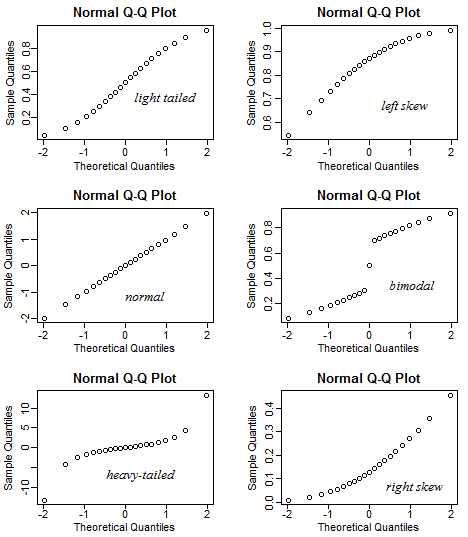
\includegraphics[width=0.6\textwidth]{figures/ch2/qqplot-tutorial}
	\caption{ How information about may be extracted from QQplots.}
	\label{fig:qqplot-tutorial}
\end{figure*}


Another way to analyze scalling characteristics is through QQplots. QQplot is a visual method to compare sample data with a specific stochastic distribution. It orders the sample data values from the smallest to largest, then plots it against the expected value given by the probability distribution function. The data sample values appear along the y-axis and the expected values along the x-axis. The more linear, the more the data is likely to be expressed by this specific stochastic distribution.

Dependent on how the plot behaves, some features of the empirical dataset compared to the theoretical can be observed. In the figure ~\ref{fig:qqplot-tutorial} is presented a summary. 


%%%%%%%%%%%%%%%%%%%%%%%%%%%%%%%%%%%%%%%%%%%%%%%%%%%%%%%%%%%%%%%%%%%%%%%%%%%%%%%%
\subsection{QoS/QoE Related Metrics}

For the point of view of a traffic generation, is interesting that the QoS and QoE metrics present similar values to the ones found in real scenarios. As stated by Magyesi and Szabó\cite{validate-trafficgen}, important QoS/QoE metrics on validation of workload tools are Roundtrip Time values (RTT), average queue waiting time and queue size. Still, on queue size, self-similar traffic consumes router buffers faster than Poisson traffic\cite{multi-player-online-game-self-similarity}.


\section{Conclusions}

In this chapter, we review and discussed some fundamental concepts of our research: network traffic generators, network traffic modeling, and network traffic generators validation. In the section ~\ref{sec:traffic-gen} we surveyed types of traffic generators, and a comparison between its considerable variability of features. It helped us to summarize and have a deep understanding of what is available today for use, and define its gaps. Also, it helped us to see find what tools and frameworks are possible for us to use. In the section ~\ref{sec:modeling-traffic} create a brief overview putting together efforts on network traffic modeling and realistic traffic generation. On modeling, we made a short historical summary of some critical points, and on practical traffic generation, we discussed some reference tools.


%%%%%%%%%%%%%%%%%%%%%%%%%%%%%%%%%%%%%%%%%%%%%%%%%%%%%%%%%%%%%%%%%%%%%%%%%%%%%%%%
%\section{An short overview of some Network emerging scenarios}

%\textcolor{red}{TODO}

%%%%%%%%%%%%%%%%%%%%%%%%%%%%%%%%%%%%%%%%%%%%%%%%%%%%%%%%%%%%%%%%%%%%%%%%%%%%%%%%
%\subsection{SDN: Software Defined Networks}

%\textcolor{red}{TODO}

%%%%%%%%%%%%%%%%%%%%%%%%%%%%%%%%%%%%%%%%%%%%%%%%%%%%%%%%%%%%%%%%%%%%%%%%%%%%%%%%
%\subsection{NFV: Network Function Virtualization}

%\textcolor{red}{TODO}

%For NFV instrumentation and benchmark, there are still few works aiming this gap. \cite{instrumentation-framework-nfv} create a web-based framework for NFV instrumentation in bare-metal and embedded level, but the source code is not provided. \cite{nfv-benchmarking-fault} implement some use cases of NFVIs (Network Function Virtualization Infrastructures) based on fault injection. \cite{nfpa-paper} implement an open-source tool, called NFPA, focusing on benchmarking of Network Functions. 

%%%%%%%%%%%%%%%%%%%%%%%%%%%%%%%%%%%%%%%%%%%%%%%%%%%%%%%%%%%%%%%%%%%%%%%%%%%%%%%%
\chapter{Architecture and Methods}\label{ch:architecture}
%%%%%%%%%%%%%%%%%%%%%%%%%%%%%%%%%%%%%%%%%%%%%%%%%%%%%%%%%%%%%%%%%%%%%%%%%%%%%%%%

In this chapter, we will present our tool which aims to fill the gaps addressed in chapter~\ref{ch:introduction}. \textit{SIMITAR} is an acronym for \textbf{\textit{SnIffing, ModellIng, and TrAffic geneRation}}\footnote{A Scimitar or Scymitar is curved sword, originating in the Middle East\cite{scymitar-sword}.}. This acronym summarizes its operation.
SIMITAR is a traffic generator able to \textbf{\textit{learn}} features of real traffic automatically, and reproduce synthetic traffic similar to the original. It records a model for the traffic in an \acrshort{XML}\footnote{Extensible Markup Language (XML) is a markup language that defines rules for storing and processing hierarchical data\cite{web-xml}.} file we call the \textit{Compact Trace Descriptor}(CTD file) as input-data SIMITAR can use, \textit{pcap} files or real-time captures. 

\begin{figure*}[ht!]
    \centering
    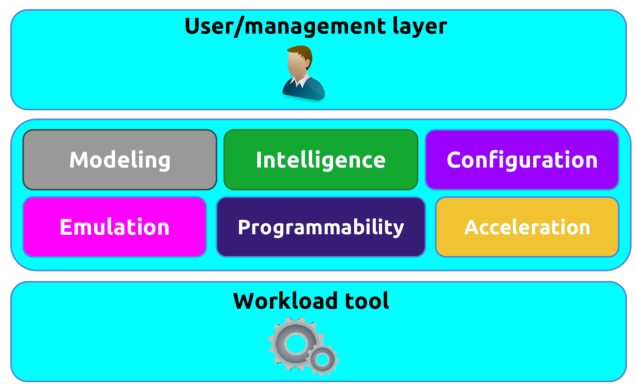
\includegraphics[height=2.4in]{figures/ch1/layer-diagram}
    \caption{ Architecture conceptual idea: a toll to automatize many tasks on traffic modelling and generation.}
    \label{fig:layer-diagram}
\end{figure*}

In figure~\ref{fig:layer-diagram} we abstract our stated concepts in a layer model diagram. Our tool works as an intermediate layer which offers traffic \textbf{\textit{modeling}}, \textbf{\textit{configuration}}, \textbf{\textit{emulation}}, and \textbf{\textit{programmability}}. In the figure, we also include packet acceleration\footnote{Packet acceleration is a concept introduced by DPDK\cite{web-dpdk}, which means kernel by-pass. Packet acceleration optimizes the packet processing, and therefore traffic generation, enabling higher throughput rates.}, which is not implemented yet but discussed as future work, in chapter~\ref{ch:conclusion}.  We are going to refer to the underlying workload tool as the packet generator engine and it is used via API by SIMITAR. 

We are also introducing the concept of \textit{programmability}. The user may create custom traffic, creating the \textit{Compact Trace Descriptor}, following its template. The idea is that he or she can create custom traffic in a platform agnostic way, without having to study any documentation, and implement any script or program.  Using a component methodology, we uncouple the packet generation, from the data collection and parameterization process. We developed it using the factory design pattern\footnote{Design patterns are abstractions that aim to help the implementation and systems structuring\cite{web-design-patterns}.} to make the extension easy for any packet generator engine. 

We abstract its whole operation cycle in figure~\ref{fig:cycle-of-operation}. Our tool collects packet data from live captures or pcap files. It then breaks down the traffic into flows and uses the data to generate parameters for our traffic model. Finally, SIMITAR provides these parameters to a packet generator engine and controls the packet injection.

% cycle of operation
\begin{figure*}[ht!]
        \centering
        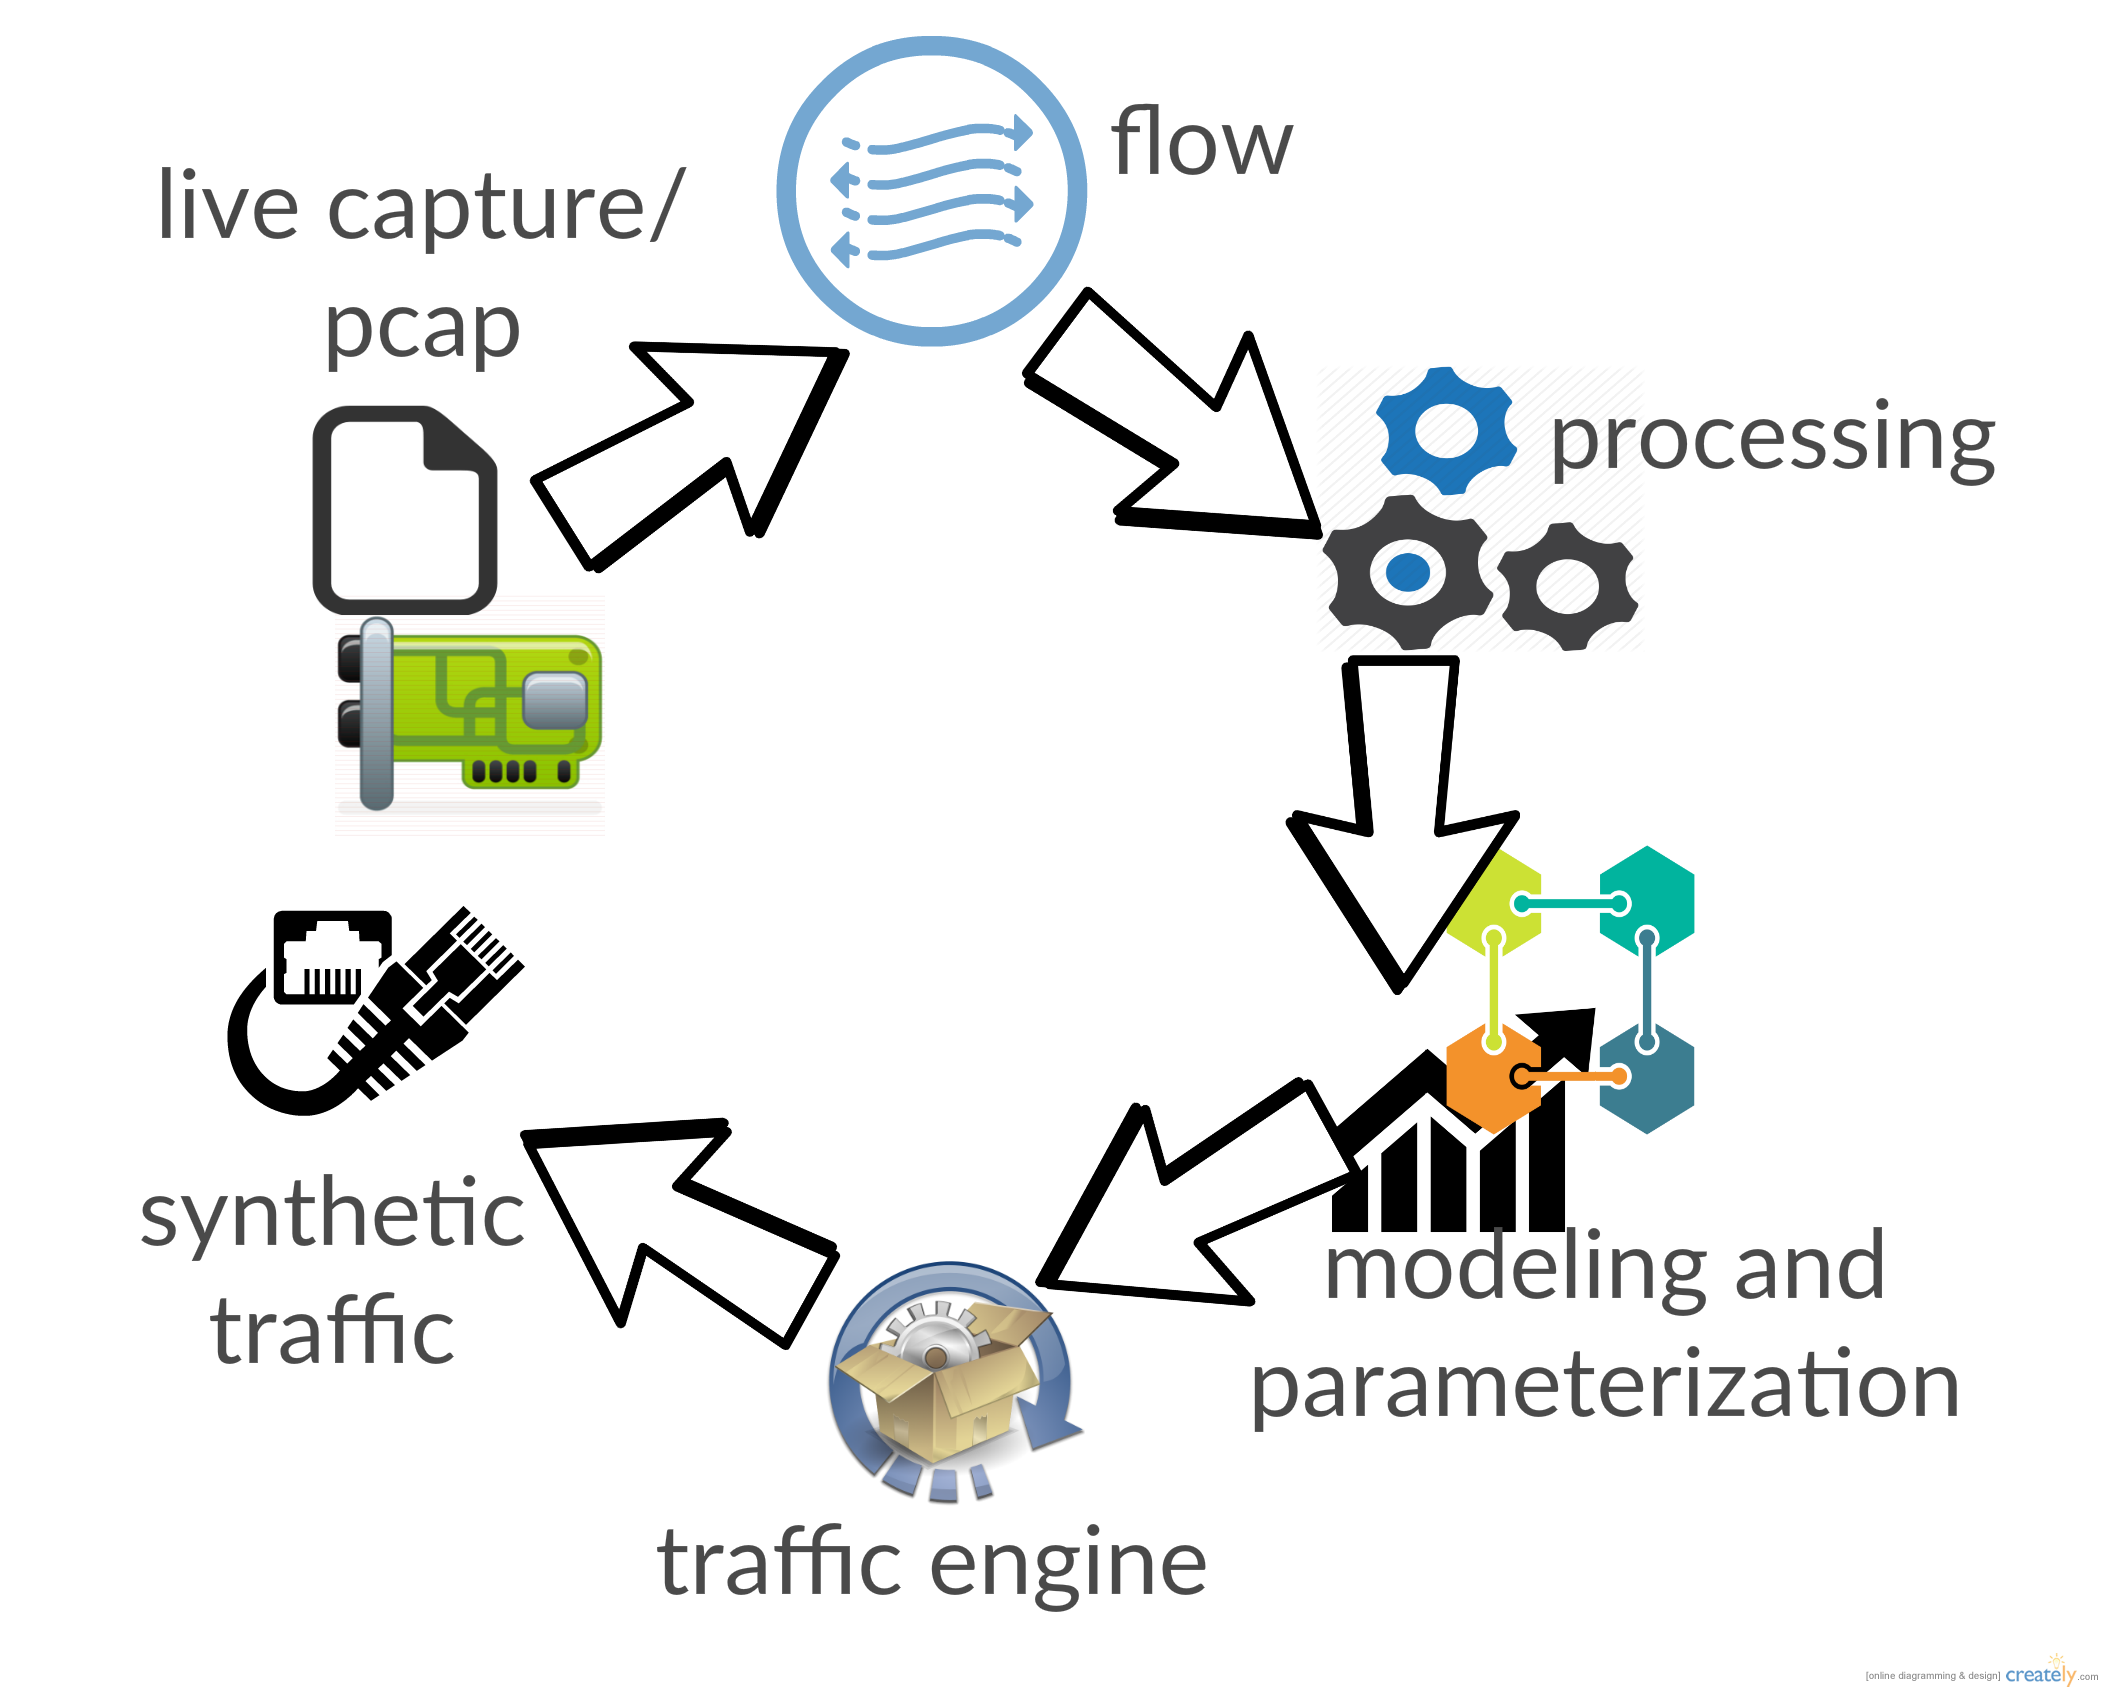
\includegraphics[height=3.0in]{figures/ch3/digram-project-cycle}
        \caption{This figure represents an operation cycle of SIMITAR, emphasizing each main step: sniffing, flow classification, data storing, data processing and fitting, model parameterization,  and synthetic traffic generation.}
    \label{fig:cycle-of-operation}
\end{figure*}

%%%%%%%%%%%%%%%%%%%%%%%%%%%%%%%%%%%%%%%%%%%%%%%%%%%%%%%%%%%%%%%%%%%%%%%%%%%%%%%%
\section{SIMITAR Architecture Overview}

The SIMITAR architecture is shown in figure~\ref{fig:architecture}. It is composed of four components: a \textbf{\textit{Sniffer}}, an \textbf{\textit{SQLite database}}, a \textbf{\textit{Trace Analyzer}}, a \textbf{\textit{Flow Generator}}. We describe each part below.

% component diagram and module design
\begin{figure*}[ht!]
        \centering
        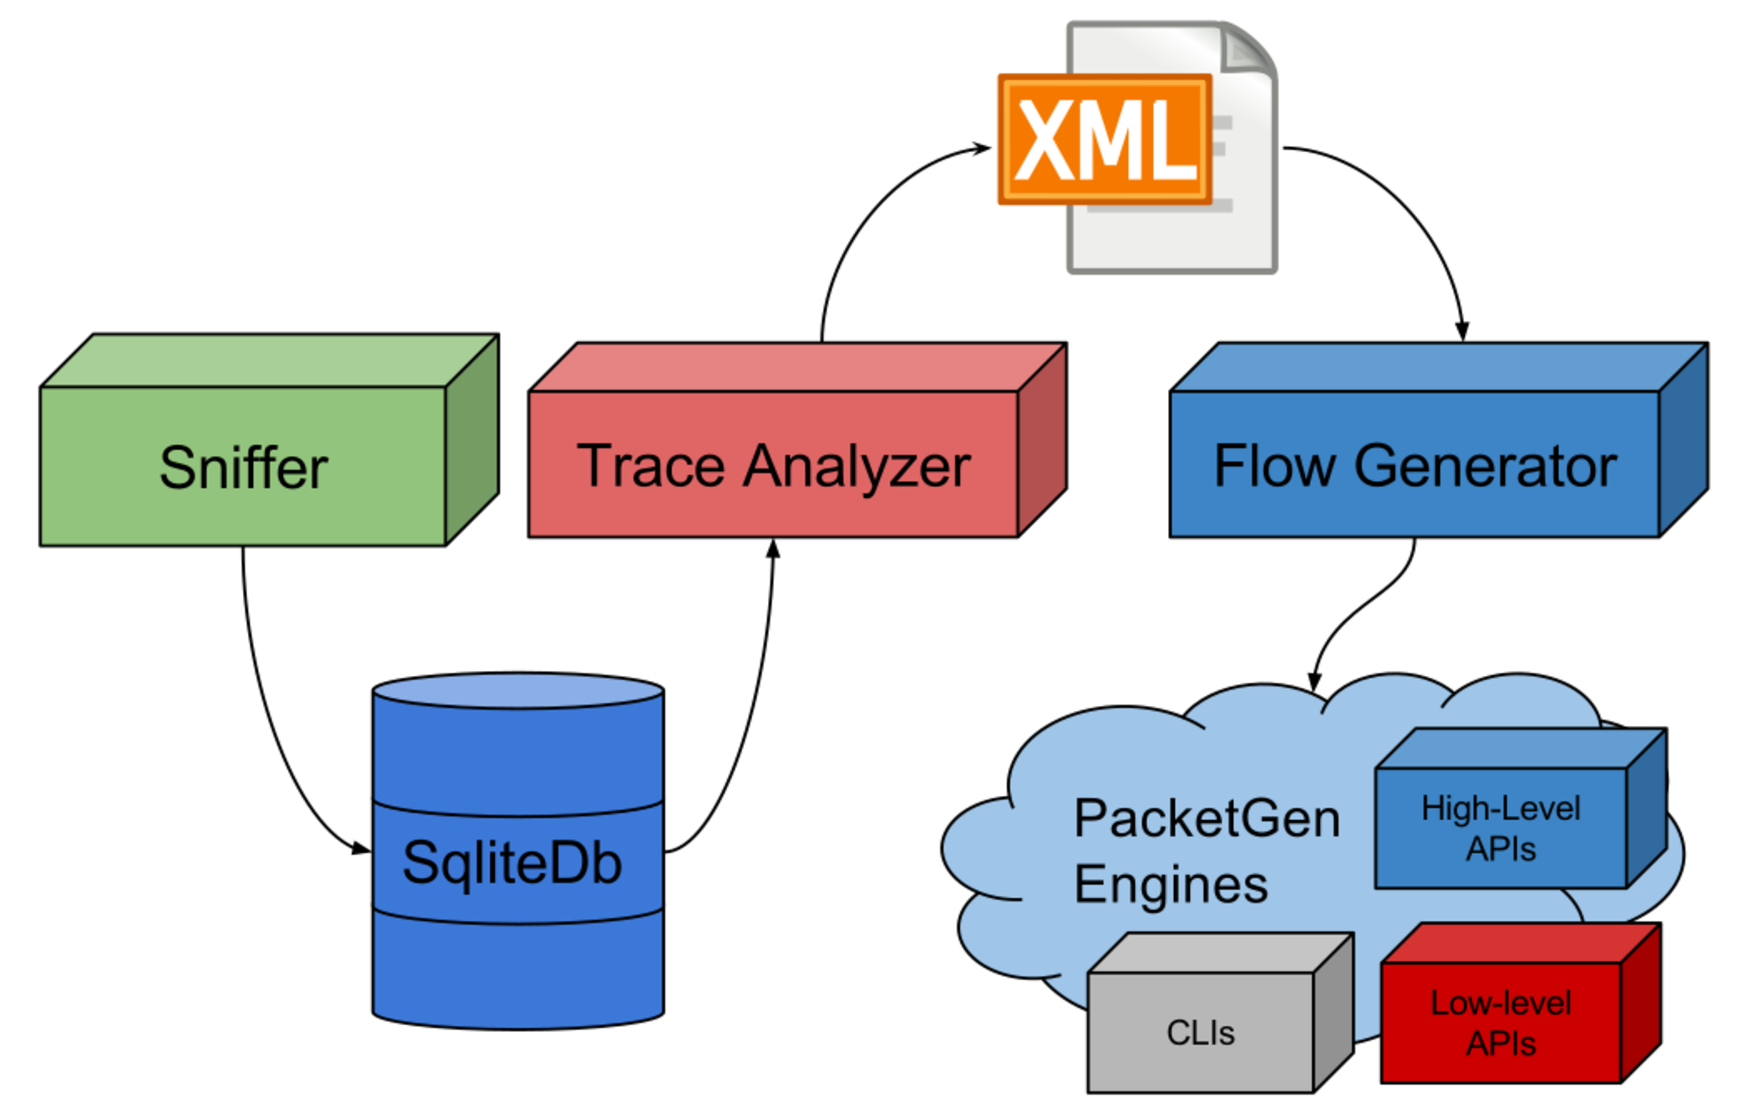
\includegraphics[height=2.7in]{figures/ch3/architecture-diagram}
        \caption{Architecture of SIMITAR}
    \label{fig:architecture}
\end{figure*}

%%%%%%%%%%%%%%%%%%%%%%%%%%%%%%%%%%%%%%%%%%%%%%%%%%%%%%%%%%%%%%%%%%%%%%%%%%%%%%%%
\section{ \textit{Sniffer} }


A sniffer is a tool that can intercept and analyze internet packets from a given network interface. Our \textit{Sniffer} component collects network traffic data and classifies it into flows, storing it on an SQLite database. It uses header field matches to classify the flows, such as in SDN switches\cite{sdn-survey}. The fields used  are:

\begin{itemize}
\item Link Protocol
\item Network Protocol
\item Network Source and Destination Address
\item Transport Protocol
\item Transport Source and Destination Port
\end{itemize}


\begin{figure*}[ht!]
        \centering
        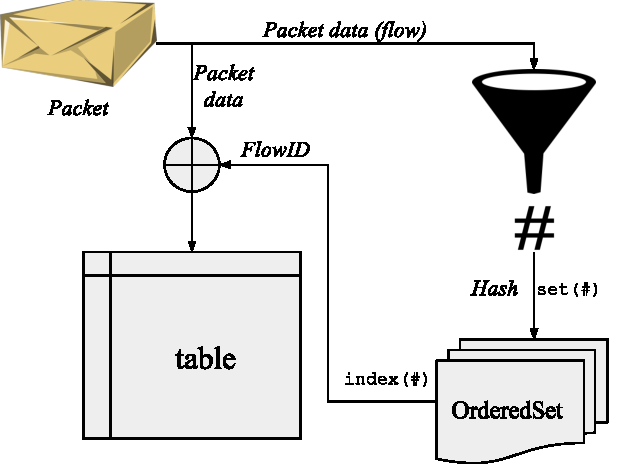
\includegraphics[height=2.5in]{figures/ch3/sniffer-classifier}
        \caption{SIMITAR's sniffer hash-based flow classification}
    \label{fig:sniffer}
\end{figure*}



We implemented the first version of this component in Shell Script (Bash). Tshark\cite{web-tshark} was used to extract header fields, and Awk to match the flows, and Sed/Awk to create the SQLite queries. This version was too slow to operate in real time on ethernet interfaces. On the other hand, this approach was fast to implement and enabled the implementation of the other components. The second and current version is in Python. This version used Pyshark\cite{web-pyshark} as a sniffer library.

The \textit{Sniffer} has a data structure we developed called \textit{OrderedSet}. A set is a list of elements with no repetition but does not keep track of the insertion order. Our \textit{OrderedSet} does. Also, it uses a 64 bit hash function from the \acrshort{FNV}\footnote{The collision probability of a good 64 bits hash function in a table with 10000 items is about of $2.71e-12$.} family. The listed header fields are inputs for a hash function. The hash value is added to the ordered set which returns its order (index on the \textit{OrderedSet}). We chose its value as packet \acrshort{flowID}.

%c++ http://ideone.com/F0V42m
As future improvements for this component, we propose a more efficient implementation in C++ and data visualization for the collected data. In this way, we can optimize packet processing. We discuss this in more depth in chapter~\ref{ch:conclusion}.

%%%%%%%%%%%%%%%%%%%%%%%%%%%%%%%%%%%%%%%%%%%%%%%%%%%%%%%%%%%%%%%%%%%%%%%%%%%%%%%%
\section{ \textit{SQLite database} }

\begin{figure*}[ht!]
        \centering
        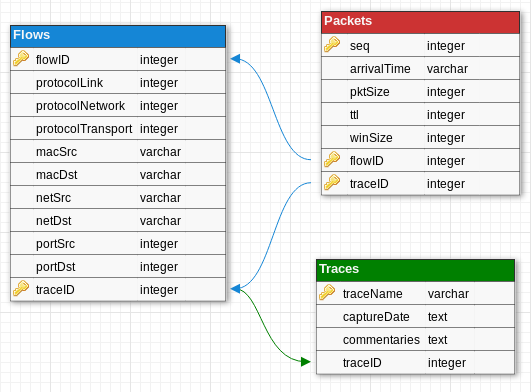
\includegraphics[height=3.0in]{figures/ch3/database-relational-model}
        \caption{SIMITAR's SQLite database relational model}
    \label{fig:simitar-database}
\end{figure*}




The database stores the collected raw data from the traces for further analysis. The \textit{Sniffer} records data on it and the  \textit{Trace Analyzer} reads. We choose an SQLite database because according to its specifications\cite{web-sqlite}, it fits our purposes well. It is simple and suitable for an amount of data smaller than terabytes. In figure~\ref{fig:simitar-database}, we present the relational model of our database, which stores a set of features extracted from packets, along with the flowID calculated by the \textit{Sniffer} component.


%%%%%%%%%%%%%%%%%%%%%%%%%%%%%%%%%%%%%%%%%%%%%%%%%%%%%%%%%%%%%%%%%%%%%%%%%%%%%%%%
\section{ \textit{Trace Analyzer} }


This module is the core of our project. It creates a trace model via the analysis of the collected data. The \textit{Trace Analyzer} has the task to learn these features from raw trace data (stored in the SQLite database) and generate an XML file to store a parameterized model. A \textit{Compact Trace Descriptor} (CTD) acts as a human and machine-readable file, which describes a traffic trace through a set of flows, each of them represented by a set of parameters, such as header information and analytical models. In figure~\ref{fig:CTD-diagram} we show a directory diagram of a CDT file. It has many flow fields, and each one contains each estimated parameter . We will now describe how we constructed it.


\begin{figure}
\centering
\subfloat[]{
  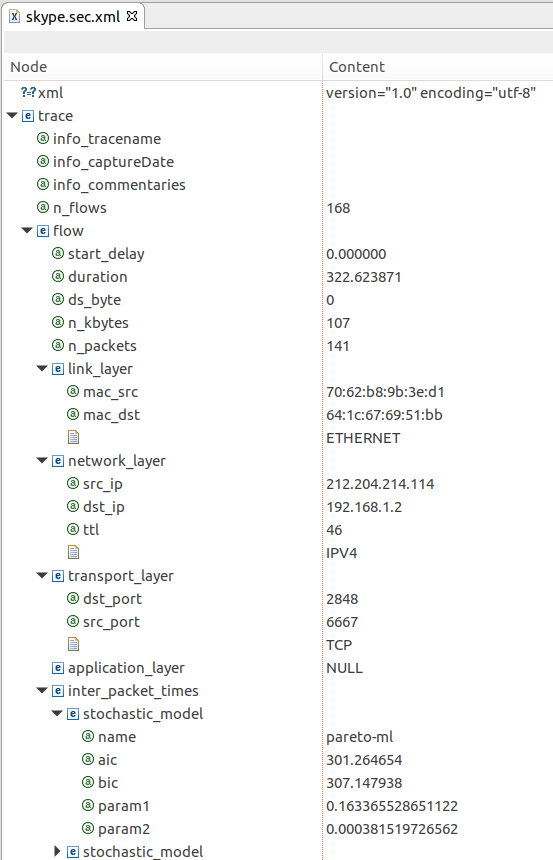
\includegraphics[height=4.in]{figures/ch3/cdt1}
}
\subfloat[]{
  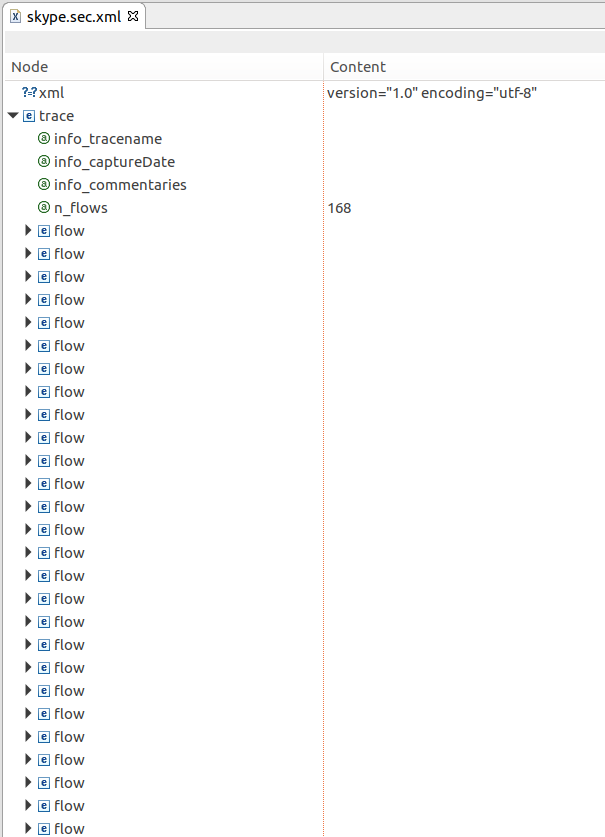
\includegraphics[height=4.in]{figures/ch3/cdt2}
}
\caption{Directory diagram of the schema of a Compact Trace Descriptor (CDT) file. On the left, we present a dissected flow, and on the right a set of flows.}
\label{fig:CTD-diagram}
\end{figure}


%%%%%%%%%%%%%%%%%%%%%%%%%%%%%%%%%%%%%%%%%%%%%%%%%%%%%%%%%%%%%%%%%%%%%%%%%%%%%%%%
\subsection{Flow features}

We measured some flow-features directly from data. They are:

\begin{itemize}
\item Flow-level properties like duration of flow, start delay, number of packets per flow, number of KBytes per flow;
\item Header fields, like protocols, QoS fields, ports, and addresses.
\end{itemize}

Each one of these parameters is unique to each flow. Other features like packet-size distribution and inter-packet times follow probability distributions. To represent these characteristics, we used sets of stochastic-based models.

%%%%%%%%%%%%%%%%%%%%%%%%%%%%%%%%%%%%%%%%%%%%%%%%%%%%%%%%%%%%%%%%%%%%%%%%%%%%%%%%
\subsection{Inter-Packet Times}


\begin{figure*}[ht!]
    \centering
    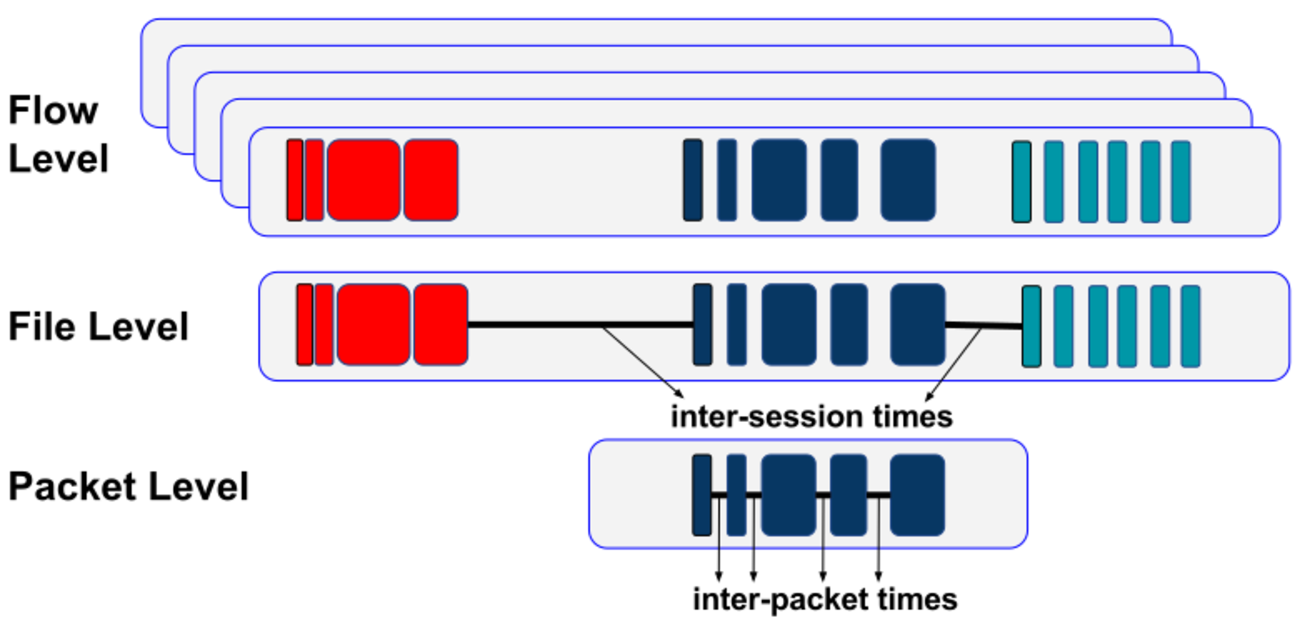
\includegraphics[height=2.0in]{figures/ch3/modified-harpoon-model}
    \caption{The schema of the modified version of the Harpoon algorithm we adopt on SIMITAR.}
    \label{fig:modified-harpoon-model}
\end{figure*}


To represent inter-packet times, we adopted a modified version of the Harpoon’s traffic model. An in-depth explanation of the original model can be found at  \cite{harpoon-paper} and \cite{harpoon-validation}. Harpoon uses a definition of each level, based on the measurement of \acrshort{SYN} and \acrshort{ACK} TCP flags. It uses TCP flags (SYN) to classify packets at different levels, naming their file, session, and user level. We chose to estimate these values, based on inter-packet times only. The distinction is made based on the time delay between packets. For our purposes, the advantage of our strategy is that the evaluation of the packet-train is not attached to a specific header field so that we can define packet trains for any flow. We illustrate this behavior in figure~\ref{fig:modified-harpoon-model}.

In our algorithm, we defined three different layers of data transference to model and control: \textit{file}, \textit{session}, and \textit{flow}. For SIMITAR, a file is a sequence of consecutive packets transmitted continuously, without a long interruption of traffic. A file can be, for example, packets from a download, a UDP connection or a single \acrshort{ICMP} echo packet. The session-layer refers to a sequence of multiple files transmitted between a source and a destination, belonging to the same flow. The flow level refers to the conjunction of flows, as classified by the \textit{Sniffer}. Now, we will explain SIMITAR operation for each layer.

In the \textbf{flow-layer}, the \textit{Trace Analyzer}  loads the flow arrival times from the database and calculates the inter-packet times within the flow context. At the session layer, we used a deterministic approach for evaluating file transference time and times between files: ON/OFF times sequence for packet trains. We chose a deterministic model because in this way we can express diurnal behavior. We developed an algorithm called \texttt{calcOnOff} that estimates these times. It also determines the number of packets and bytes transferred for each file. Since the ON times will serve as input for actual traffic generators, we defined a minimum acceptable time for on periods equal to 100 ms. ON times can be arbitrary and small, and they could be incompatible with acceptable ON periods for traffic generators. Also in the case of just one packet, the ON time would be zero. So  a minimum acceptable time was set to solve these issues. The OFF times, on the other hand, are defined by the constant \texttt{session\_cut\_time}\footnote{In the code it is called \texttt{DataProcessor::m\_session\_cut\_time} }. If the time between two packets of the same flow is greater than \texttt{session\_cut\_time}, we consider them belonging to a different file, so this time is a session OFF time. In this case, we use the same value of the constant \textit{Request and Response timeout} of Swing\cite{swing-paper} for the \texttt{session\_cut\_time}: 30 seconds. The control of ON/OFF periods in the traffic generation is made by the \textit{Flow Generator} component\footnote{This control is made by the class \texttt{NetworkFlow}}.

In the \textbf{file-layer}, we modeled the inter-packet times at the file level. We selected all times smaller than \texttt{session\_cut\_time} 9, and all files within the same flow were considered to follow the same model. We delegated the control of the inter-packet times to the underlying packet generator engine. We ordered them, from the best to the worst. Currently, we are using eight different stochastic functions parameterizations. We display each of them in table~\ref{tab:parameterizations-sumary} .

\begin{table}[ht!]
	\centering
	\caption{Functions and parameterizations used by SIMITAR}
		\begin{tabular}{c c c c}
			\toprule
			\textbf{Function} & Linear Regression & Maximum Likelihood & Empirical\footnotemark \\
			\midrule
			Weibull         & $\checkmark$    &                  &                  \\
			Normal             &                  &                  &  $\checkmark$    \\
			Exponential      & $\checkmark$    &                  &  $\checkmark$    \\
			Pareto          & $\checkmark$    & $\checkmark$    &                  \\
			Cauchy          & $\checkmark$    &                  &                  \\
			Constant          &                 &                  & $\checkmark$    \\
			\bottomrule
		\end{tabular}
		\label{tab:parameterizations-sumary}
\end{table}
\footnotetext{Empirical estimation, by calculation of the avarge, and standard deviation} 


From the functions presented in the first column in table~\ref{tab:parameterizations-sumary}, Weibull, Pareto, and Cauchy are heavy-tailed (and self-similar processes). However, if the flow has less than 30 packets, just the constant model is evaluated. It is because numerical methods gave poor results if the data sample is small. We sorted these models according to the Akaike Information Criterion (AIC) as default\cite{sourcesonoff-paper}\cite{bic-aic-comparision}. This methodology is explained in-depth in chapter~\ref{ch:modeling-evaluation} and illustrated in figure 10.  All these constants and modes of operation are modifiable via command-line options.

\begin{figure*}[ht!]
    \centering
    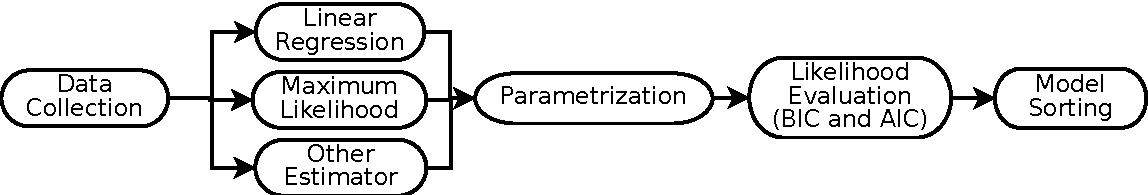
\includegraphics[height=0.9in]{figures/ch3/simitar-parametrization}
    \caption{Diagram of parameterization and model selection for inter-packet times and inter-file times.}
    \label{fig:model-parameterization}
\end{figure*}

%%%%%%%%%%%%%%%%%%%%%%%%%%%%%%%%%%%%%%%%%%%%%%%%%%%%%%%%%%%%%%%%%%%%%%%%%%%%%%%%
\subsection{Packet Sizes}


Our approach for the packet size was much simpler. Since the majority of packet size distributions found in real measurements are bi-modal\cite{packet-distribution-model}\cite{sourcesonoff-paper}\cite{udp-flows-model}, we first sorted all packet sizes of flow into two modes. We defined a packet-size cut value of 750 bytes, the same value adopted by\cite{udp-flows-model}.

We knew how many packets each mode has, and then we fitted a model to it. We use three stochastic models: constant, exponential and normal. Since self-similarity does not make sense for packet-sizes, we prefered to use just the simpler models. When there was no packet for a model, we set a flag \texttt{NO\_MODEL}, and when there was only a single packet, we used the constant model. Then we calculated the $BIC$ and $AIC$ for each, but we decided to set the constant model as the first.

As is possible to see in many works\cite{packet-distribution-model} \cite{udp-flows-model}, since the standard deviation of each mode tends to be small, constant fittings give good approximations. Also, it is computationally cheaper for the traffic generated than the other models, since no calculation is needed for each packet sent. Since both $AIC$ and $BIC$ criteria will always select the constant model as the worst, we decided to ignore this.

%%%%%%%%%%%%%%%%%%%%%%%%%%%%%%%%%%%%%%%%%%%%%%%%%%%%%%%%%%%%%%%%%%%%%%%%%%%%%%%%
\subsection{ \textit{Compact Trace Descriptor} }


An example of the final result of all the methods is presented in the XML code below. The code illustrates a single flow from a \textit{Compact Trace Descriptor}(CDT) file. The inter-packet times' models are on tags "\texttt{inter\_packet\_times}" and the packet trains models on tags "\texttt{session\_times}". All the times are in seconds, and "\texttt{inf}" represents infinity. The protocol of each layer is on the data field for each tag. 


\begin{minted}[frame=single,
               framesep=3mm,
               linenos=true,
               xleftmargin=21pt,
               tabsize=4,
               fontsize=\scriptsize, 
               breaklines=true]{xml}
    <flow start_delay="0.144400" duration="317.744333" ds_byte="0" n_kbytes="40" n_packets="344">
        <link_layer mac_src="64:1c:67:69:51:bb" mac_dst="70:62:b8:9b:3e:d1">ETHERNET</link_layer>
        <network_layer src_ip="192.168.1.1" dst_ip="192.168.1.2" ttl="64">IPV4</network_layer>
        <transport_layer dst_port="2128" src_port="53">UDP</transport_layer>
        <application_layer>DNS</application_layer>
        <inter_packet_times>
            <stochastic_model name="pareto-ml" aic="-1165.310696" bic="-1157.646931" param1="0.405085202535192" param2="0.002272655895996"/>
            <stochastic_model name="pareto-lr" aic="-454.049749" bic="-446.385984" param1="0.061065000000000" param2="0.002272655895996"/>
            <stochastic_model name="weibull" aic="-246.882037" bic="-239.218273" param1="0.120355000000000" param2="0.001629000000000"/>
            <stochastic_model name="exponential-me" aic="486.370061" bic="494.033826" param1="1.340057495455104" param2="0.000000000000000"/>
            <stochastic_model name="normal" aic="1629.370900" bic="1637.034665" param1="0.746236637899171" param2="2.626808289821357"/>
            <stochastic_model name="exponential-lr" aic="3166.816047" bic="3174.479812" param1="0.009752000000000" param2="0.000000000000000"/>
            <stochastic_model name="cauchy" aic="31737.418442" bic="31745.082207" param1="0.000000000000194" param2="-3152.827055696396656"/>
            <stochastic_model name="constant" aic="inf" bic="inf" param1="0.746236637899171" param2="0.000000000000000"/>
        </inter_packet_times>
        <session_times on_times="29.22199798,73.40390396,151.84077454" off_times="30.85738373,32.42027283" n_packets="19,103,222" n_bytes="2272,12399,26689"/>
        <packet_sizes n_packets="344" n_kbytes="40">
            <ps_mode1 n_packets="344" n_kbytes="40">
                <stochastic_model name="constant" aic="inf" bic="inf" param1="120.232558" param2="0.000000"/>
                <stochastic_model name="normal" aic="2926.106952" bic="2933.788235" param1="120.232558" param2="16.941453"/>
                <stochastic_model name="exponential-me" aic="3987.126362" bic="3994.807645" param1="0.008317" param2="0.000000"/>
            </ps_mode1>
            <ps_mode2 n_packets="0" n_kbytes="0">
                <stochastic_model name="no-model-selected" aic="inf" bic="inf" param1="0.000000" param2="0.000000"/>
            </ps_mode2>
        </packet_sizes>
    </flow>
\end{minted}


%%%%%%%%%%%%%%%%%%%%%%%%%%%%%%%%%%%%%%%%%%%%%%%%%%%%%%%%%%%%%%%%%%%%%%%%%%%%%%%%
\section{ \textit{Flow Generator} }

\begin{figure*}[ht!]
    \centering
    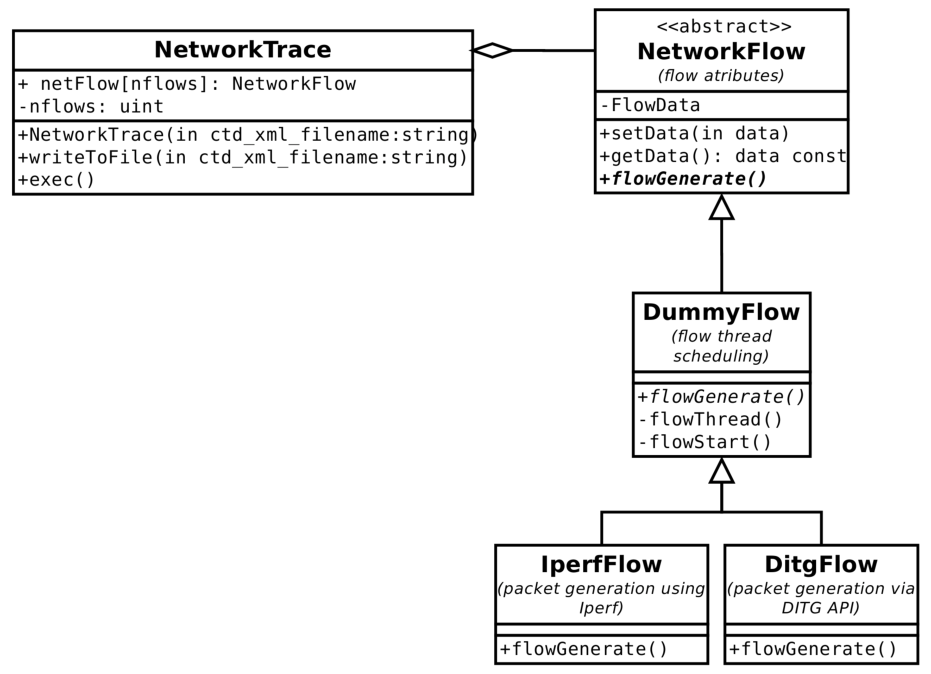
\includegraphics[height=3.0in]{figures/ch3/trace-flow}
    \caption{Class hierarchy of NetworkTrace and NetworkFlow, which enables the abstraction of the traffic generation model of the packet generation engine.}
    \label{fig:network-trace-flow-class-diagram}
\end{figure*}

\begin{figure*}[ht!]
    \centering
    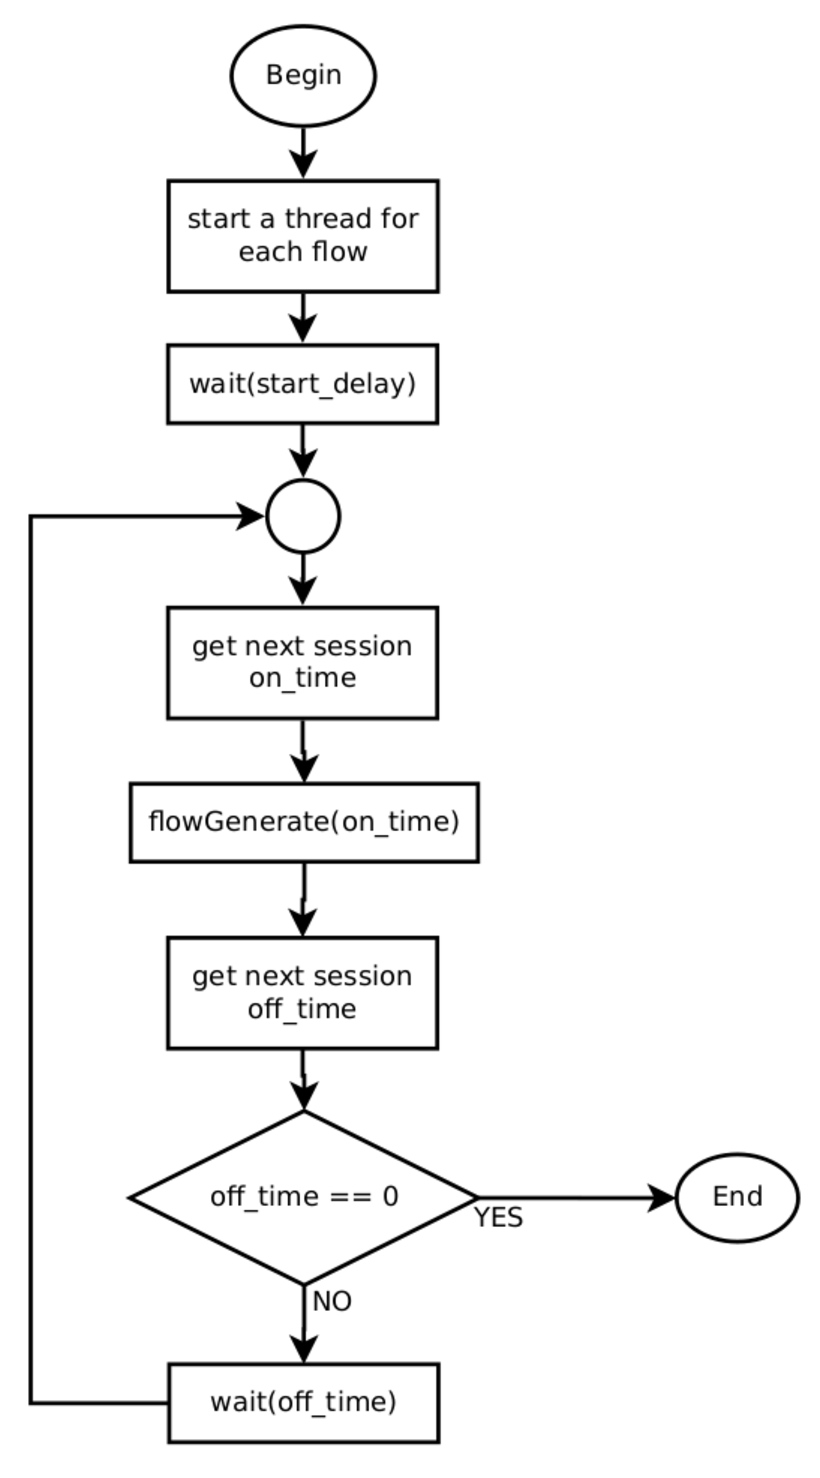
\includegraphics[height=4.5in]{figures/ch3/alg-simplified-harpoon}
    \caption{Simplified-harpoon emission algorithm}
    \label{fig:alg-simplified-harpoon}
\end{figure*}


\begin{figure*}[ht!]
    \centering
    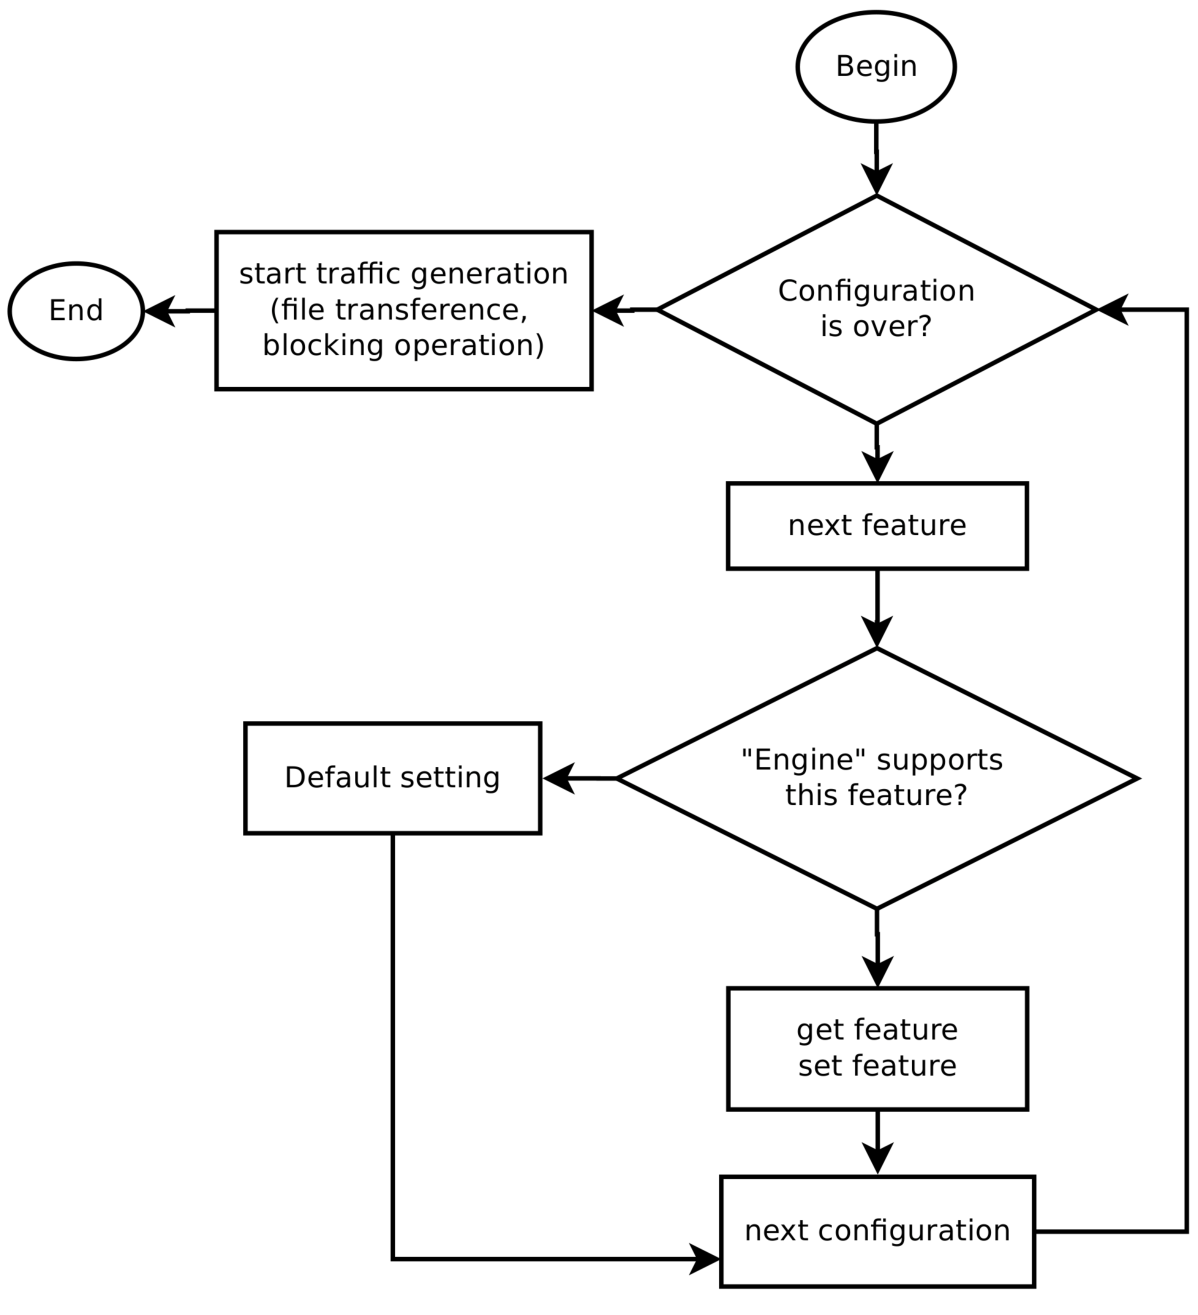
\includegraphics[height=4.0in]{figures/ch3/alg-traffic-engine-config}
    \caption{Packet engine configuration method}
    \label{fig:alg-traffic-engine-config}
\end{figure*}



The \textit{Flow Generator} handles the data on the \textit{Compact Trace Descriptor} file, and is used to retrieve parameters for traffic generation. It crafts and controls each flow in a separate thread. We have already implemented this component using Iperf and Libtins(C++ API)\cite{web-libtins} as packet generators. It must follow the class hierarchy as presented in figure~\ref{fig:network-trace-flow-class-diagram}. This component was designed using the factory design pattern, to simplify its expansion and support\footnote{
If the user wants to introduce support for a new packet generator engine, he has to implement a derived class of \texttt{DummyFlow}, such as in figure~\ref{fig:network-trace-flow-class-diagram}. In the current release of SIMITAR, we already have \texttt{IperfFlow} and \texttt{TinsFlow}, and \texttt{DitgFlow}. This new class needs to be static, and the support must be implemented on the factory \texttt{NetworkFlowFactory}.
For closed loop packet-crafters (the ones that need to establish a connection to generate traffic), two methods must be implemented: \texttt{flowGenerate()} and \texttt{server()}. \texttt{flowGenerate()} is responsible for sending a single file, as defined on de figure~\ref{fig:modified-harpoon-model}. The \texttt{server()} methods must implement the reception of $n$ files. For open-loop packet crafters (the ones whose just inject packets but do not establishes a connection), such as the one we implemented using Libtins, does not need the server-side implemented. }


This component itself is a multi-layer workload generator according to the typing introduced in chapter~\ref{ch:literature-review}\footnote{Since it works both at packet and flow level, but does not work at application level yet.}. At the flow-level, SIMITAR controls each flow using the algorithm in figure~\ref{fig:alg-simplified-harpoon}. This algorithm handles our model as defined in figure~\ref{fig:modified-harpoon-model}. This procedure is independent of the underlying packet crafting tool used. It starts a \textit{thread} for each flow in the \textit{Compact Trace Descriptor}, and then the thread sleeps for \texttt{start\_delay} seconds. The \texttt{start\_delay} is the arrival time of the first flow packet. Passed this time, it then calls the underlying packet generator tool (defined as command line argument), and passes to it the flowID, file ON time, number of packets and number of bytes to be sent (file size), and network interface. Then it sleeps until the next session OFF time. When the list of ON/OFF times from the flow is over, the thread ends.


At the packet level, SIMITAR configures the packet-generator tool to send a \textit{file}, as defined in figure~\ref{fig:modified-harpoon-model}. This method must use the available parameters, attributes and \textit{getters} to configure and generate thread-safe traffic using the method \texttt{flowGenerate()}. The \textit{file} configuration must follow figure~\ref{fig:alg-traffic-engine-config}. Down below we present a simple code of how the D-ITG API can be used to generate packet-level traffic. A more complex configuration is possible, but it serves to illustrate the procedure. We call this concept \textit{Flow Generation Programming}. Its API documentation is available at the D-ITG website\footnote{\href{http://www.grid.unina.it/software/ITG/manual/index.html\#SECTION00047000000000000000}{http://www.grid.unina.it/software/ITG/manual/index.html\#SECTION00047000000000000000}}.

\begin{minted}[frame=single,
               framesep=3mm,
               linenos=true,
               xleftmargin=21pt,
               tabsize=4,
               fontsize=\scriptsize, 
               breaklines=true]{c++}


// This implementation is just a simplified version to illustrate the procedure.
void DitgFlow::flowGenerate(const counter& flowId, const time_sec& onTime, const uint& npackets, const uint& nbytes,  const string& netInterface)
{
    // create command to generate the traffic
    std::string strCommand;
    std::string localhost = getNetworkSrcAddr(); 
    strCommand += " -t " + std::to_string(onTime); 
    strCommand += " -k " + std::to_string(nbytes / 1024);
    strCommand += " -a " + getNetworkDstAddr();
    
    // configure protocol
    if (this->getTransportProtocol() == PROTOCOL__TCP)
        strCommand += " -T TCP -D ";
    else if (this->getTransportProtocol() == PROTOCOL__UDP)
        strCommand += " -T UDP ";
    else if (this->getTransportProtocol() == PROTOCOL__ICMP)
        strCommand += " -T ICMP ";
        
    //configure inter-packet time model, just Weibull or Constant
    StochasticModelFit idtModel;
    for(uint i = 0;;i++)
    {    
        idtModel = this->getInterDepertureTimeModel(i);
        if(idtModel.modelName() == WEIBULL)
        {
            strCommand += " -W " + std::to_string(idtModel.param1()) + " " + std::to_string(idtModel.param2());
            break;
        }
        else if ( idtModel.modelName() == CONSTANT)
        {
            strCommand += " -C " + std::to_string(nbytes/(1024*onTime));
            break;
        }
    }
    
    // it uses C strings as arguments
    // it is not blocking, so it must block until finishes
    int rc = DITGsend(localhost.c_str(), command.c_str()); // D-ITG API
    usleep(onTime*10e6); // D-ITG uses miliseconds as time unity
    if (rc != 0)
    {
        PLOG_ERROR << "DITGsend() return value was" << rc ; // our log macro for erros
        exit(EXIT_FAILURE);
    }
}
\end{minted}


%%%%%%%%%%%%%%%%%%%%%%%%%%%%%%%%%%%%%%%%%%%%%%%%%%%%%%%%%%%%%%%%%%%%%%%%%%%%%%%%
\section{Network Packet Generator}


A network packet generator is a tool or library that should provide its API or script interface for the \textit{Flow Generator} component. With this engine, the user must be able to send packets and control attributes such as sending time, bandwidth, number of packets, protocols, and so on. This means, any available parameter form the \textit{Compact Trace Descriptor}.


%%%%%%%%%%%%%%%%%%%%%%%%%%%%%%%%%%%%%%%%%%%%%%%%%%%%%%%%%%%%%%%%%%%%%%%%%%%%%%%%
\section{Usage and Use Cases}


SIMITAR is composed of three main command-line applications, whose give command line access to the \textit{Sniffer}, \textit{Trace Analyzer} and \textit{Flow Generator}, respectively:
\begin{itemize}
\item \texttt{sniffer-cli.py};
\item \texttt{trace-analyzer};
\item \texttt{simitar-gen} (the actual traffic generator). 
\end{itemize}

Below we show some usage commands of SIMITAR’s components. The \texttt{sniffer-cli.py} application creates a new trace entry on the database using the command option new. Then the \textit{Trace Analyzer} can create a \textit{Compact Trace Descriptor} using the same trace entry. We can change the constants used by the \textit{Trace Analyzer} by the command line option. As a traffic generator (\texttt{simitar-gen}), SIMITAR may work as a client or a server. Working as a server is necessary for closed-loop packet-generator engines; tools that require establishing a connection before generating the traffic, such as Iperf and D-ITG. It will just work passively. Working as a client it is acting as a traffic emitter. Open loop packet-crafter tools such as Libtins do not require server operation to send the traffic. In the case of closed-loop tools, the destination IP addresses must be explicitly given in the command line by the options \texttt{--dst-list-ip} or \texttt{--dst-ip}.


\begin{minted}[frame=single,
               framesep=3mm,
               linenos=true,
               xleftmargin=21pt,
               tabsize=4,
               fontsize=\scriptsize, 
               breaklines=true]{bash}

# @ SIMITAR/, load enviroment variables
source data/config/simitar-workspace-config.sh

# @ SIMITAR/sniffer/, execute to sniff the eth0 interface, and create a trace entry called "intrig" in the database
./sniffer-cli.py new intrig live eth0

# @ SIMITAR/sniffer/, execute this command to list all traces recorded in the database
./sniffer-cli.py list

# @ SIMITAR/trace-analyzer/, execute this command to create two Compact Trace Descriptors, called intrig.ms.xml and intrig.sec.xml. The first is parameterized using milliseconds, and de second uses seconds as time unity.
./trace-analyzer --trace intrig

# @ SIMITAR/simitar-gen/, execute these commands to generate traffic using the intrig.sec.xml compact trace descriptor. It is stored at the directory "../data/xml/". 
# Libtins
./simitar-gen --tool tins --mode client --ether eth0 --xml ../data/xml/intrig.sec.xml 
# Iperf
./simitar-gen --tool iperf --mode client --ether eth0 --xml ../data/xml/intrig.sec.xml --dst-ip 10.0.0.2
./simitar-gen --tool iperf --mode server --ether eth0 --xml ../data/xml/intrig.sec.xml

\end{minted}


\begin{figure*}[ht!]
    \centering
    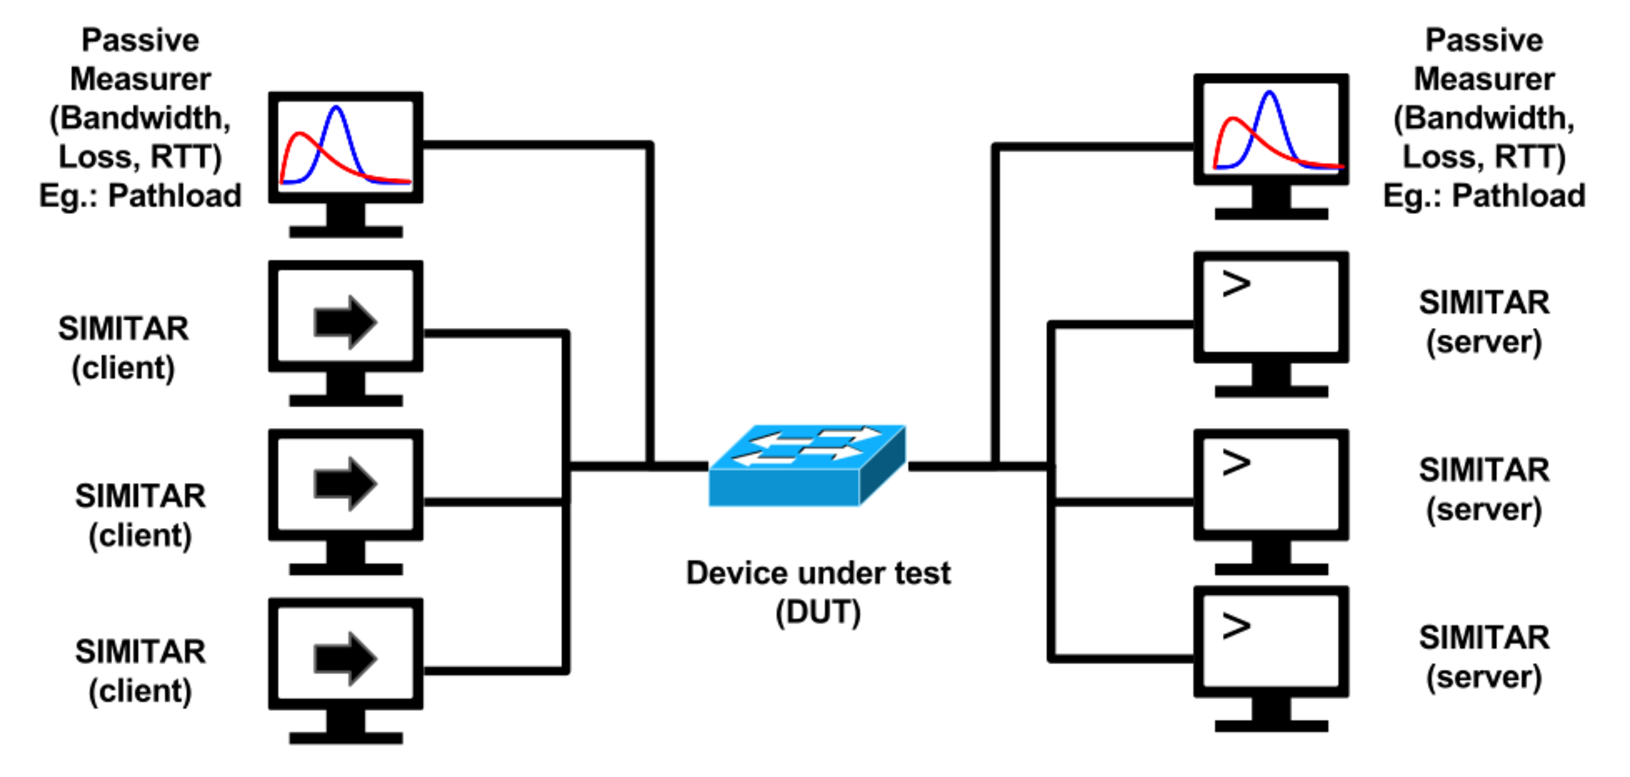
\includegraphics[height=2.4in]{figures/ch3/use-case}
    \caption{Use case example of SIMITAR}
    \label{fig:use-case}
\end{figure*}



Figure~\ref{fig:use-case} shows an example of a use case. A device under test can be stressed using a combination of traffic generated by many clients and server pairs. In the case of an open-loop packet generator tool (such as in the Libtins implementation), the servers and clients pairs are not necessary. Using passive network measures, such as Pathload\cite{web-pathload} and pathChirp\cite{swing-paper}\cite{web-pathchirp}, it is possible to measure statistics from the device under tests.

%%%%%%%%%%%%%%%%%%%%%%%%%%%%%%%%%%%%%%%%%%%%%%%%%%%%%%%%%%%%%%%%%%%%%%%%%%%%%%%%
\chapter{Traffic Modeling and Algorithms}\label{ch:modeling-evaluation}
%%%%%%%%%%%%%%%%%%%%%%%%%%%%%%%%%%%%%%%%%%%%%%%%%%%%%%%%%%%%%%%%%%%%%%%%%%%%%%%%


In this chapter, we are going to go into deep details on some implementations and modeling approaches mentioned in the last chapter. In the first section, we are going to discuss our methodology for modeling inter packet-times, and proof that it is a good choice. But before putting our hands on the problem, we need to precisely define what we want. We abstract our ideas in the bullets below:

\begin{itemize}    
    \item Given a set of empiral inter-packet times, we want to parametrize not only one, bua a set of "candidates" stochastic functions to describe it
    \item We want to know, analitically,  which of these candidates is the best, avoiding human analysis;
    \item We need a proof that our choosen analifical analysis is good or not to describe inter-packet times.
\end{itemize}

In the second section, we will describe and discuss the methods we used to estimate the packet-trains sizes (ON/OFF times), and to do the application classification. The calculation of the packet trains periods in our model is deterministic. The \textit{compact trace descriptor} stores the same ON and OFF times from each flow from the original traffic trace. The application classification is made by a match table of transport protocols and ports. 

\section{Inter Packet Times Modelling}

\subsection{About Inter packet time and packet trains modeling}

There are many works devoted to studying the nature of the Ethernet traffic\cite{selfsimilar-ethernet}. Classic Ethernet models used Poisson related processes to express generation of traffic. Initially, it makes sense since a Poisson process represents the probability of events occur with a known average rate, and independently of the last occurence\cite{selfsimilar-ethernet} \cite{book-poisson}. But studies made by Leland et al.\cite{selfsimilar-ethernet} showed that the Ethernet traffic has a self-similar and fractal nature. Even if they can represent the randomness of Ethernet traffic, simple Poisson processes can't express traffic "burstiness" on a long-term time scale, such as traffic "spikes" on long-range "ripples". These characteristics are an indication of the fractal and self-similar nature of the traffic, that usually we express by distributions with infinite variance, called heavy-tailed. Heavy-tail means that a stochastic distribution is not exponentially bounded\cite{sourcesonoff-paper}. Examples of heavy-tailed functions are Weibull, Pareto, Cauchy.  But heavy-tailed function may guarantee self-similarity, but not necessarily they will ensure other features like good correlation and same average packet rate.

There many consolidate works that investigate the nature of the internet traffic\cite{selfsimilar-ethernet}\cite{analysis-self-similar}\cite{stochartic-selfsimilar}\cite{selfsimilar-highvariability}\cite{multi-player-online-game-self-similarity}, and many others on the modelling of stochastic functions for specific scenarios\cite{estimation-renewal-function-ethernet-traffic}\cite{modelling-of-self-similar}\cite{empirical-interarrival-study}\cite{modeling-concurrent-heavy-tailed}\cite{optimal-scheduling-of-heavy-tailed-traffic}\cite{modelling-of-self-similar}. But not as many on model choice automation\cite{sourcesonoff-paper}.

There are plenty of works in the literature which proposes new processes and methodologies for modeling times between packets and packet trains. Fiorini \cite{modeling-concurrent-heavy-tailed} presents a heavy-tailed ON/OFF model, which tries to represent traffic generated by many sources. The model emulates a multiple source power-tail Markov-Modulated (PT-MMPP) ON/OFF process, where the ON times are power-tail distributed. They achieve analytical performance measurements using Linear Algebra Queueing Theory. Kreban and Clearwater\cite{hierarchical-dynamics-interarrival-times} presents a model for times between job submissions of multiple users over a supercomputer. They show that the Weibull probability functions can express well small and high values of inter-job submission times. They also tested exponential, lognormal and Pareto distributions. Exponential distribution couldn't represent long-range values because it fell off too fast and Pareto was too slow. Lognormal fit well small values, but was weak on larger ones. Kronewitter\cite{optimal-scheduling-of-heavy-tailed-traffic} presents a model of scheduling traffic of many heavy-tail sources. On his work, he uses many Pareto sources to represent the traffic. To estimate the shape parameter $\alpha$ they use linear regression.

In this chapter, we propose a method automatically by software. We estimate many stochastic functions through many methodologies and select the best model through the AIC computation\cite{bic-aic-comparision}. Since generating random can be costly and have a bias, depending on the seed generator, we avoid these problems since our method is analytical. We show the traffic traces we are going to use in this chapter, and in the rest of our work, and then present or selected method for parameterization and fitting choice. To test our criteria quality, we define a validation method, based on cross-validations made by simulations.

% citations
% \cite{bivariate-gamma-distribution-arrival}
% \cite{bic-aic-comparision}
% \cite{sourcesonoff-paper}
% \cite{modelling-of-self-similar}
% \cite{realtime-detection-dos}
% \cite{traffic-modelling-matlab}
% \cite{trasmission-failure}
% \cite{improvement-approaches-modeling}

\subsection{Modelling Methodology}

We start defining also define the \textit{pcaps} datasets we are going to use in the rest of this text. We will use for datasets, and for reproduction purposes, three are publicly available. 
The first is a lightweight Skype capture, found in  Wireshark wiki\footnote{https://wiki.wireshark.org/}, and can be found at \href{https://wiki.wireshark.org/SampleCaptures}{https://wiki.wireshark.org/SampleCaptures}. The file name is \texttt{SkypeIRC.cap}, and we call it \textit{skype-pcap}.

The second is a CAIDA\footnote{http://www.caida.org/home/}{http://www.caida.org/home/} capture, and can be found at  \href{https://data.caida.org/datasets/passive-2016/equinix-chicago/20160121-130000.UTC}{https://data.caida.org/datasets/passive-2016/equinix-chicago/20160121-130000.UTC}. Access to this file need login, so you will have to create an account and wait for approval first. The pcap's file name is \texttt{equinix-chicago.dirB.20160121-135641.UTC.anon.pcap.gz}. We call it \textit{wan-pcap}.

The third we capture in our laboratory LAN, through a period of 24 hours. It was captured firewall gateway between our local and external network. Along with other tests, We intend to verify diurnal behavior on it. That means a high demand of packets during the day and a small in the night. We call it \textit{lan-firewall-diurnal-pcap}.

%2nd-review
The fourth is a capture of a busy private network access point to the Internet, available online on TCPreplay website \footnote{ \href{http://tcpreplay.appneta.com/wiki/captures.html}{http://tcpreplay.appneta.com/wiki/captures.html}}, called \texttt{bigFlows.pcap}. We will refer to it \textit{lan-gateway-pcap}.


%In this chapter we will evaluate our proposed method for data modeling of inter-packet times.  We will present curves obtained by our prototype (implemented in Gnu Octave\footnote{\href{https://www.gnu.org/software/octave/}{https://www.gnu.org/software/octave/}}) that shows in detail how each step works. After explaining this process, we will present an evaluation method of our results, analyzing to analyze its quality. After this, we give some details of how we convert code from Octave to C++ and its benefits on time execution. All code used in this section is available on our GitHub page.%, on the directory \texttt{Prototypes}. 


%Along with these datasets, we will use two subpcaps from the originals. The first, \textit{skype-flowburst-pcap}, is a burst of a single HTTP flow from \textit{skype-pcap}. It can be obtained from Wireshark using the filter \texttt{(ip.src\_host==172.16.133.25) \&\& (ip.dst\_host==74.125.170.42) \&\& (tcp.dstport==80) \&\& (tcp.srcport==63378) \&\& (frame.time\_relative>30.0) \&\&( frame.time\_relative<50.0)}. The second, \textit{caida1s-pcap} is a trace with the first second from \texttt{wan-pcap}.


%2nd-review
We summarize our process of modeling inter-packet times at the figure~\ref{fig:model-parameterization}. We collect a set of inter-packet times from an actual traffic capture. Then, we estimate a set of parameters for stochastic functions, using different methodologies. Then, from these parametrized models, we determine which best represent our data set, using the measure of quality AIC (Akaike information criterion). We also calculate another ratio of quality called BIC (Bayesian information criterion), for comparison of results. In this chapter, we present our results obtained on our prototype implemented in Octave\footnote{ \href{https://www.gnu.org/software/octave/}{https://www.gnu.org/software/octave/}}. 

Currently, we are modeling:

\begin{itemize}
    \item Weibull distribution, using linear regression, through the Gradient descendant algorithm;
    \item Normal distribution, using direct calculation of the average and the standard deviation of the inter-packet times from the dataset;
    \item Exponential distribution, using linear regression, through the Gradient descendant algorithm. We refer to this distribution as Exponential(LR);
    \item Exponential distribution, using a rate estimation form the dataset. We refer to this distribution as Exponential(Me);
    \item Pareto distribution, using linear regression, through the Gradient descendant algorithm. We refer to this distribution as Pareto(LR);
    \item Pareto distribution, using the maximum likelihood method. We refer to this distribution as Pareto(MLH);
    \item Cauchy distribution, using linear regression, through the Gradient descendant algorithm;
\end{itemize}

%\textcolor{red}{TODO: Explciar quais dados são armazenados na base de dados e por que. Explicar como os dados são classificados, e modelados, e os parametros gerados. Citar métodos utilizado para parametrização, como calculo da média, maximmum likelihood e regressão linear. Apredentar o diagrama da ultima apresentação. Apresentar as equações utilizadas. Com esses dados bem como os plots dos dados linearizados, da corvergencia do custo e o fitting da CDF. Apresentar uma tabela com o valor do BIC e AIC para cada fitting. (Vai ficar muito grande a sessão)}

% In probability theory and statistics, the exponential distribution (a.k.a. negative exponential distribution) is the probability distribution that describes the time between events in a Poisson process, i.e., a process in which events occur continuously and independently at a constant average rate. It is a particular case of the gamma distribution. It is the continuous analog of the geometric distribution, and it has the crucial property of being memoryless. In addition to being used for the analysis of Poisson processes, it is found in various other contexts.

Now we will give a brief explanation our three procedures: Linear Regression (with the  Gradient descendant algorithm), direct estimation, and maximum likelihood. Some observations must be made. Since the time samples resolution used were of $10^{-6}$s, all values equal to zero were set to  $5\cdot10^{-8}$s, to avoid division by zero. To avoid divergence in tangent operation used in the linearization of the Cauchy function, we floor-limited and upper-limited the inter-packet CDF  values by  $10^{-6}$ and $0.999999$, respectively. We implemented this prototype using Octave. We upload the code on GitHub, for reproduction purposes\footnote{\href{https://github.com/AndersonPaschoalon/ProjetoMestrado/tree/master/Tests/PrototypeDataProcessor}{https://github.com/AndersonPaschoalon/ProjetoMestrado/tree/master/Tests/PrototypeDataProcessor}}

%We go deep into details explaining the methods on the appendix ~\ref{ap:revision-probability}, and present the mathematical demonstrations on appendix~\ref{ap:revision-probability}. 

\subsubsection{Linear regression (Gradient descendant)}

Linear regression is a method for estimating the best linear curve in the format:

\begin{equation}
y = ax + b
\end{equation}

to fit a given data set. We can use linear regression to estimate parameters of a non-linear curve expressing it on a linear format. For example, the Weibull CDF for $t > 0$ is:

\begin{equation}
F(t|\alpha, \beta) = F(t) = 1 - e^{-(t/\beta)^{\alpha}}
\end{equation}

Manipuling the equation:
\begin{equation}
\alpha\ln{(t)} - \alpha\ln{(\beta)} = \ln{(-\ln{(1 - F(t))})}
\end{equation}


If we call $x = \ln{(t)}$ and $y = \ln{(-\ln{(1 - F(t))})}$, we found a linear equation, where $a = \alpha$ and $b = -\alpha\ln{(\beta)}$. Having in hands a estimation of the empirical CDF of our data samples, we apply the $x$ and $y$ definitions to linearize the data. 

Using the gradient descendant, we find an estimation of the linear coefficients $\hat{a}$ and $\hat{b}$. Using the inverse function of linear factors, we see the Weibull estimated parameters $\hat{\alpha}$ and $\hat{\beta}$.

\begin{equation}
\alpha = a
\end{equation}

\begin{equation}
\beta = e^{-(b/a)}
\end{equation}

The gradient descendent consists in minimizing a cost function $J(\theta)$. We explain this procedure in the appendix ~\ref{ap:revision-probability}. In the figure~\ref{fig:linearization} we present as examples, the linearized data for the inter arrivals from the \textit{skype-pcap}, and in the figure ~\ref{fig:cost} the cost convergence. In the appendix ~\ref{ap:aditional-plots}, a complete set of these figures is presented.

Applying the inverse equations of the linear coefficients ($\hat{\alpha} = \hat{a}$ and $\hat{\beta} = e^{-(\hat{b}/\hat{a})}$) \footnote{The hat symbol ( $ \widehat{} $ ) for the estimated parameters}, we are able to estimate the Weibull distribution parameters. We can summarize this procedure, in these steps:
\begin{enumerate}
\item Linearize the stochastic CDF function F(t).
\item Apply the linearized $y = y(F(t))$ and  $x = x(t)$ on the empirical CDF and times datasets, respectively. 
\item Use Gradient Descendant algorithm to find linear coefficients $a$ and $b$.
\item Apply the inverse equation of the linear coefficients, to determine the stochastic function parameters.
\end{enumerate}

In the parameters estimation (step 4), there is an exception, since the Pareto scale ($t_{m}$) is defined by the minimum time. In the table~\ref{tab:linearization-sumary} we present a summary of the used equations in the procedure. In this notation, the subscript $i$ means that it must be applied to every value measured empirically. The hat( $\widehat{}$ ) indicates an estimated value for a parameter. 

\begin{table}[h!]
    \centering
    \caption{Linearized functions, and parameters estimators, used by the linear regression}
    \label{tab:linearization-sumary}
    \begin{tabular}{llllll}
        \hline
        Function    & Linearized $x$     & Linearized $y$                    & \multicolumn{2}{l}{Parameters Estimator}                               &  \\
        \hline
        Cauchy      & $x_i = t_i$        & $y_i = \tan{(\pi(F(t_i) - 1/2))}$ & $\hat{\gamma} = \frac{1}{\hat{a}}$ & $\hat{t_0} = - \frac{\hat{b}}{\hat{a}}$                      &  \\
        Exponential & $x_i = t_i$        & $y_i = \ln{(1 - F(t_i))})$        & \multicolumn{2}{l}{$\hat{\lambda} = -\hat{a}$}                                              &  \\
        Pareto      & $x_i = \ln{(t_i)}$ & $y_i = \ln{(1 - F(t_i))}$         & $\hat{\alpha} = -\hat{a} $         & $\hat{x_{m}} = \min_{i = 0, ..., m}\{x_{i}\}$ &  \\
        Weibull     & $x = \ln{(t)}$     & $y = \ln{(-\ln{(1 - F(t))})}$     & $\hat{\alpha} = \hat{a}$                 & $\hat{\beta} = e^{-(\hat{b}/\hat{a})}$                                   & \\
        \hline
    \end{tabular}
\end{table}



\begin{figure}[ht!]
\centering
\subfloat[Linearized interarrival data]{
  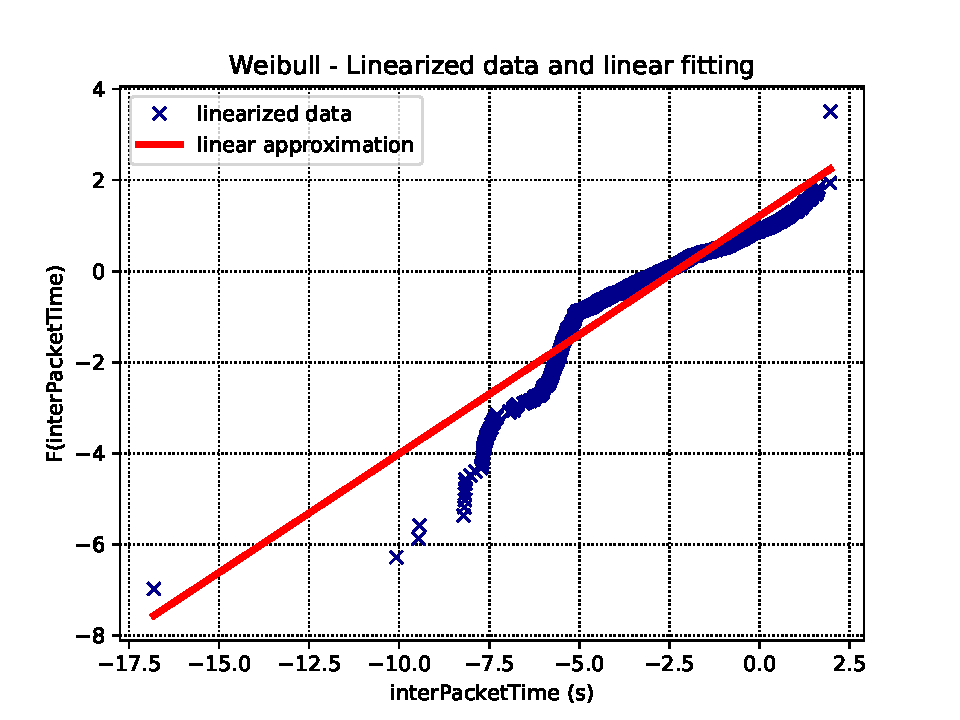
\includegraphics[height=50mm]{figures/ch4/Skype_Weibull_-_Linearized_data_and_linear_fitting}
  \label{fig:linearization}
}
%\hspace{0mm}
\subfloat[Cost function of the linear regression]{
  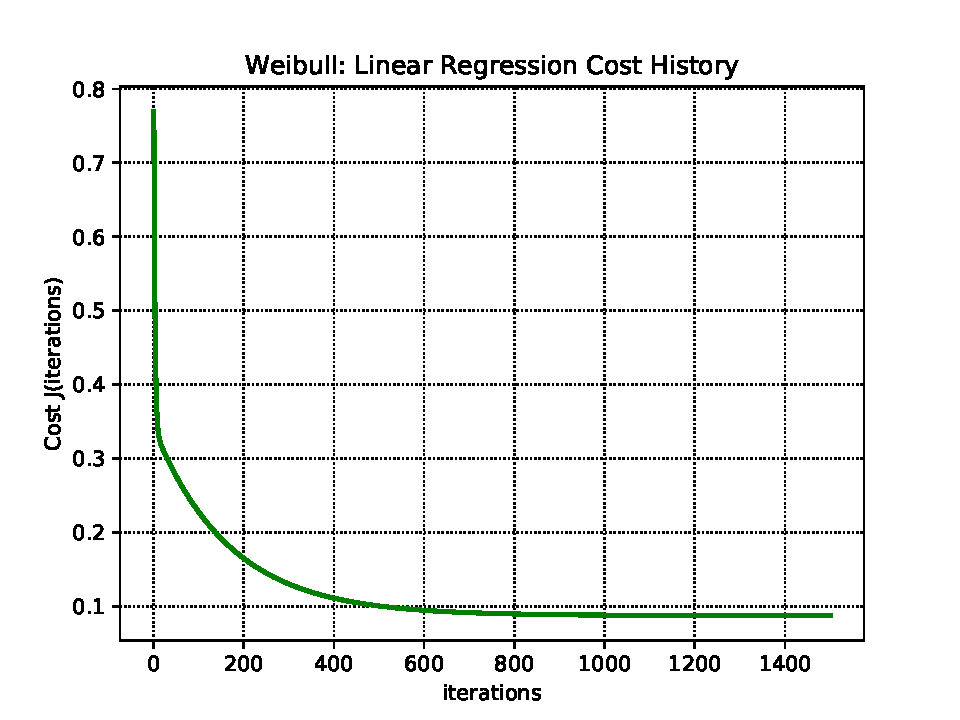
\includegraphics[height=50mm]{figures/ch4/Skype_Weibull_-_Cost_J(iterations)_convergence}
  \label{fig:cost}
}
\label{fig:linearization-cost}
\caption{Linearized data and cost function of weibull linear regression}
\end{figure}



\subsubsection{Direct Estimation}

%2nd-review
The expected value $E(X)$ and variance $Var(X)$ of a random variable $X$ of some distributions are closely related to its parameters. Since the average $\bar{\mu}$ and its standard deviation $\bar{\sigma}$ are in general good approximations for the expected value and variance, we use them to estimate parameters.

%2nd-review
Following the notation presented at table~\ref{tab:distributions-equations}, we have for the normal distribution:
\begin{equation}
(\hat{\mu}, \hat{\sigma} = (\bar{\mu}, \bar{\sigma})
\end{equation}

%2nd-review
For the exponential distribution $E(X) = \frac{1}{\lambda}$, therefore we have:
\begin{equation}
\hat{\lambda} = \frac{1}{\hat{\mu}}
\end{equation} 

\subsubsection{Maximum Likelihood}


The maximum likelihood estimation, is a method for estimation of parameters, winch maximizes the likelihood function. We explain in details this subject in the Appendix A. Using this method for the Pareto distribution, it is possible to derive the following equations the its parameters:

\begin{equation}
\hat{x_{m}} = \min_{i = 0, ..., m}\{x_{i}\}
\end{equation} 

\begin{equation}
\hat{\alpha} = \frac{n}{ \sum_{i = 0}^{m}(\ln{(x_{i}) - \ln(\hat{x_{m}})})  }
\end{equation} 

where $m$ is the sample size.


\subsection{Modelling Method Validation}

To see if our criterion of parameter selection is can find which is the best model, we define a validation methodology. 
We generate a vector with the same size form the original, with randomly generated data through our model estimation. Then we compare it with the original sample, trough four different metrics, all with a confidence interval of 95\%:

\begin{itemize}
\item Correlation between the sample data and the estimated model (Pearson's product-moment coefficient);
\item Hurst exponent;
\item Mean inter-packet time;
\item Standard deviation of inter-packet times.
\end{itemize}

The Pearson's product-moment coefficient, or simply correlation coefficient,  is an expression of the dependence or association between two datasets. Its value goes from -1 to +1. +1 means a perfect direct linear correlation. -1 indicates perfect inverse linear correlation. 0 means no linear correlation. So, as close the result reaches 1, more similar are the inter-packet times to the original values. To estimate it, we use the Octave's function \texttt{corr()}.

As explained before in the chapter~\ref{ch:literature-review}, the Hurst exponent is meter self-similarity and indicates the fractal level of the inter-packet times. As close the result is from the original, more similar is the fractal level of the estimated samples from the original. To determine this value, we use the function \texttt{hurst()} from Octave, which uses rescaled range method.
Finally we measure the mean and the standard deviation (as a measure of the dispersion), using the Octave's functions \texttt{mean()} and \texttt{std()}. We also present some \textit{QQplots}, to visually compare the random-generated data and the original dataset. 

As close the correlation, Hurst exponent, average and the standard deviation is from the original dataset, the better is model fitting. Also, analyzing the average, we can see if a particular modeling procedure tends to be more penalized for the values close, or far from zero. This means that if the average inter-packet time tends to be smaller or higher compared to the original. 

With these results in hands, we can see if AIC and BIC are reasonable criteria for model selection for inter-packet times. To quantitatively check it, we define a cost function based on the correlation, Hurst exponent and mean. We exclude the standard deviation, because the Hurst exponent being a meter of the fractal level, also capture information about the desired dispersion of the data. So, for comparing all these results, we defined a cost function $J$, based on the randomly generated data values.

Being $Cr$ the vector of correlations ordered from greater to the smaller, let $Me$ and $Hr$ defined by the absolute difference between average and hurt exponent of the estimated values and the original dataset. Both are ordered from the smaller to the greatest values. Letting $\phi(V, M)$ be an operator which gives the position of a model $M$ in a vector $V$, we define the cost function $J$ as:


\begin{equation}
J(M) = \phi(Cr, M) + \phi(Me, M) + \phi(Hr, M)
\end{equation}

The smaller is the cost $J$, the best is the model. Then we compare the results achieved by AIC and BIC, and $J$.

\subsection{Modelling Results}

%%%%%%%%%%%%%%%%%%%%%%%
% Logscale Skype
%%%%%%%%%%%%%%%%%%%%%%%
\begin{figure}[ht!]
\centering
\subfloat[Chauchy]{
  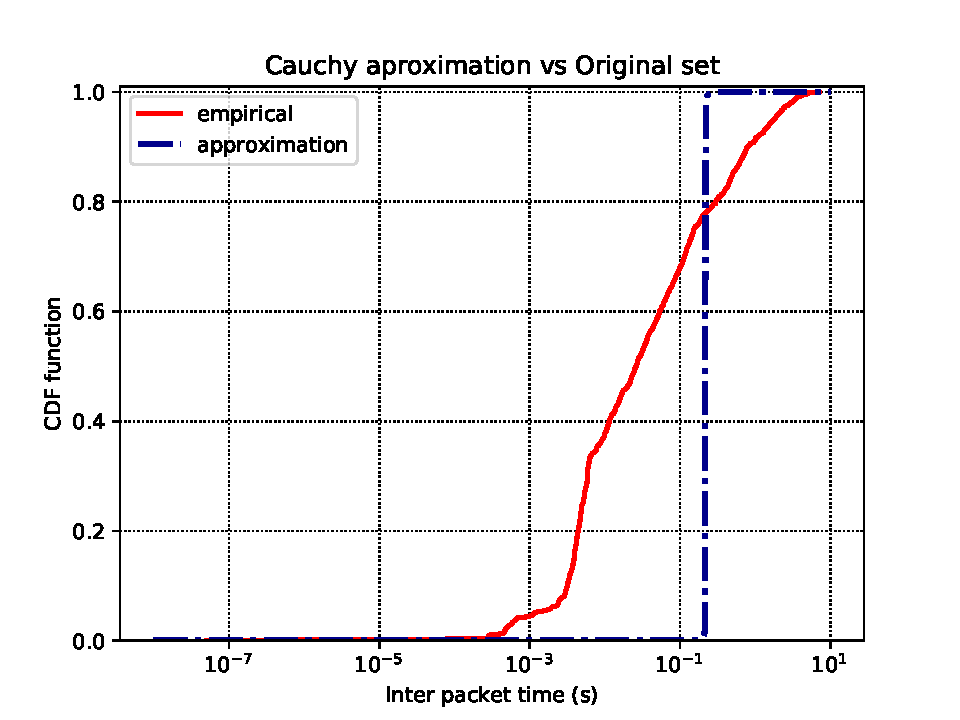
\includegraphics[width=62mm]{figures/ch4/Skype_Log_-_Cauchy_aproximation_vs_Original_set}
}
\subfloat[Exponential(LR)]{
  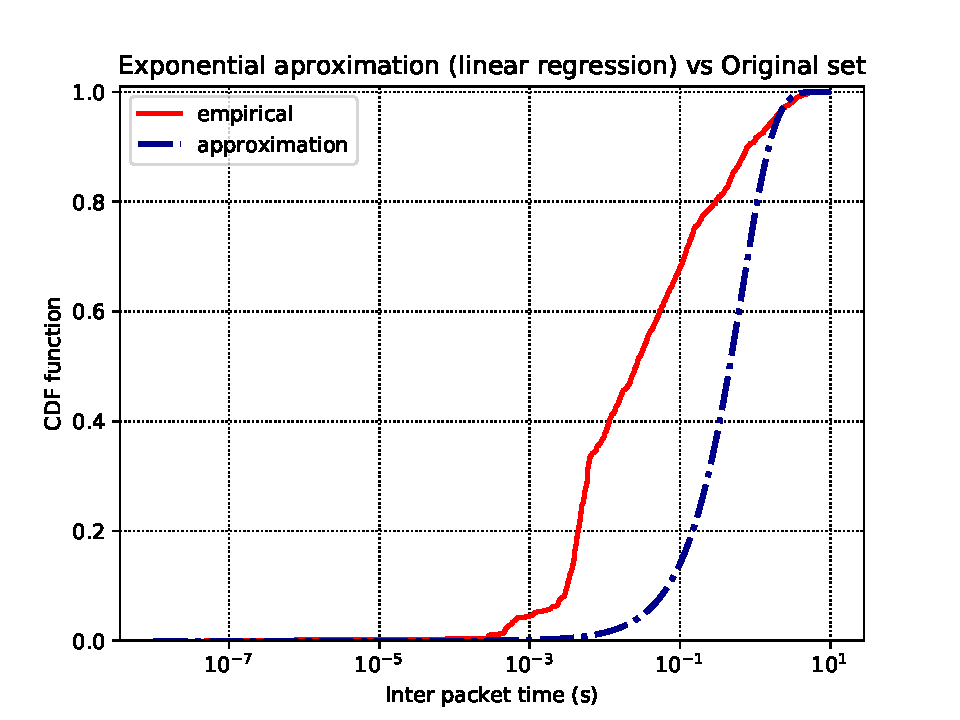
\includegraphics[width=62mm]{figures/ch4/Skype_Log_-_Exponential_aproximation_(linear_regression)_vs_Original_set}
}
\hspace{0mm}
\subfloat[Exponential(Me)]{
  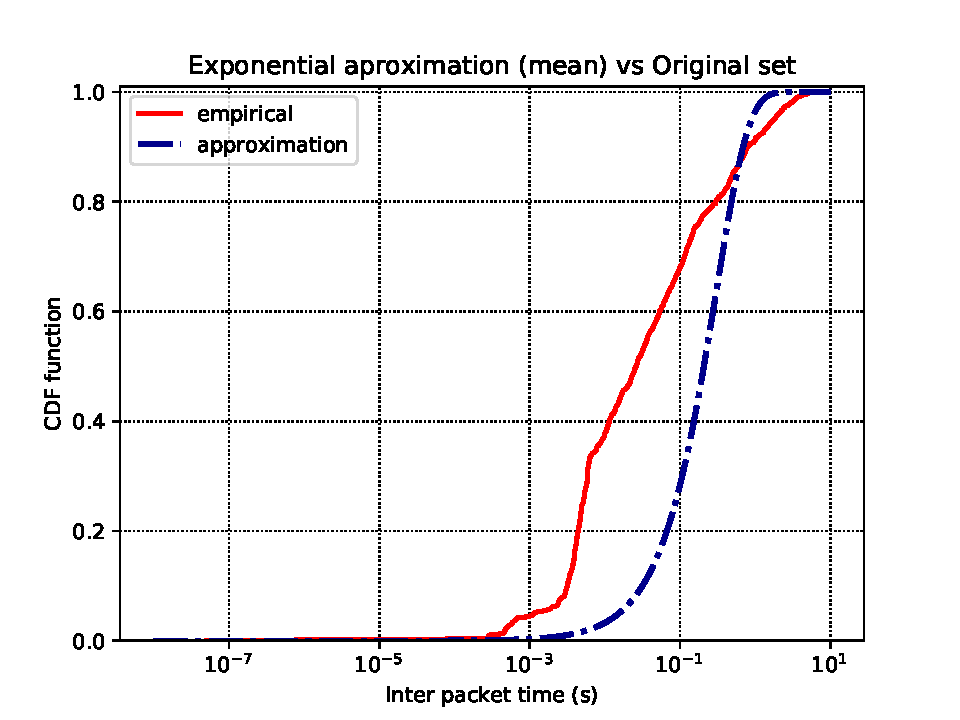
\includegraphics[width=62mm]{figures/ch4/Skype_Log_-_Exponential_aproximation_(mean)_vs_Original_set}
}
\subfloat[Normal]{
  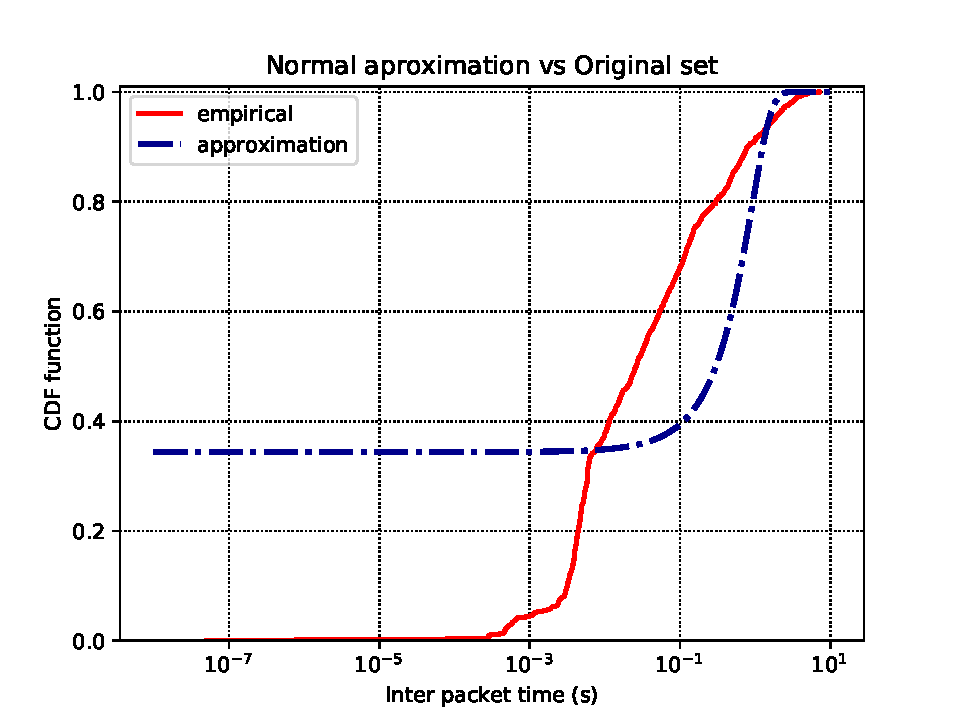
\includegraphics[width=62mm]{figures/ch4/Skype_Log_-_Normal_aproximation_vs_Original_set}
}
\hspace{0mm}
\subfloat[Pareto(LR)]{
  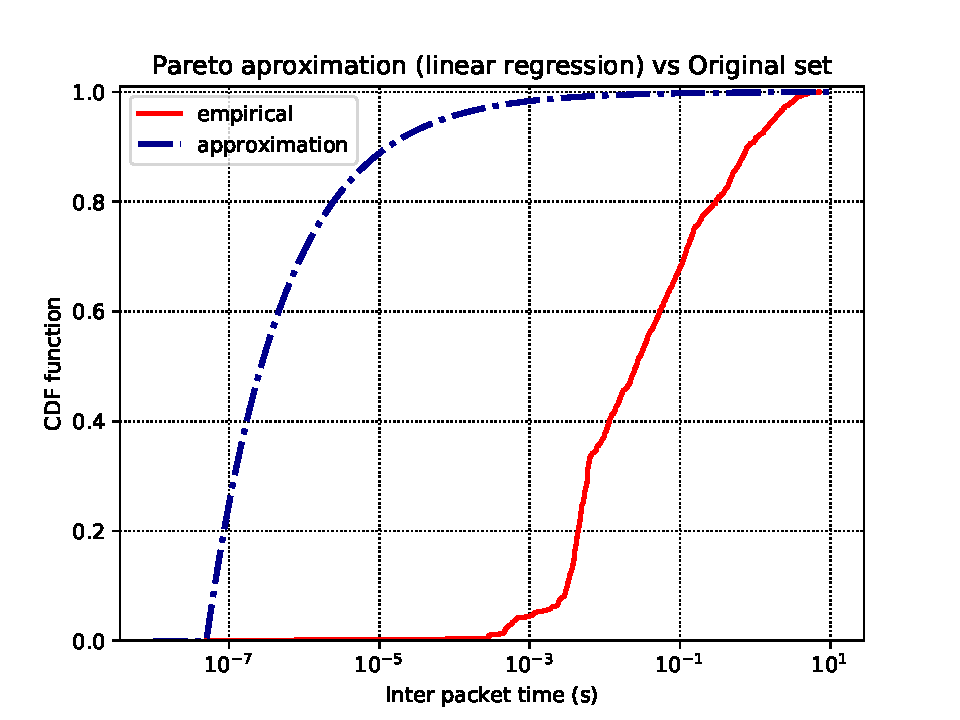
\includegraphics[width=62mm]{figures/ch4/Skype_Log_-_Pareto_aproximation_(linear_regression)_vs_Original_set}
}
\subfloat[Pareto(MLH)]{
  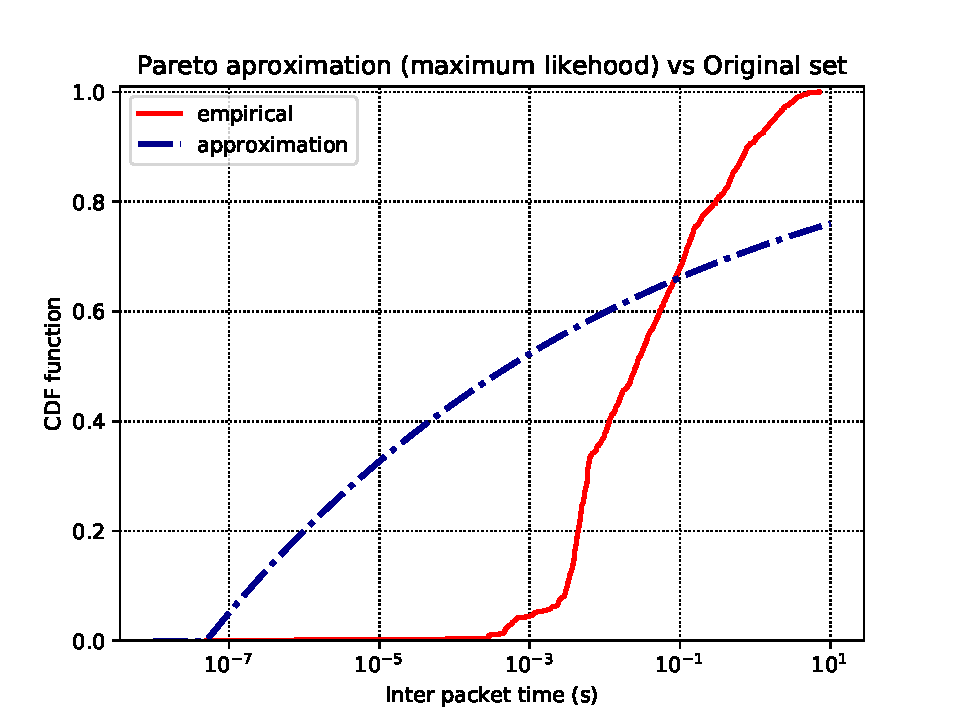
\includegraphics[width=62mm]{figures/ch4/Skype_Log_-_Pareto_aproximation_(maximum_likehood)_vs_Original_set}
}
\hspace{0mm}
\subfloat[Weibull]{
  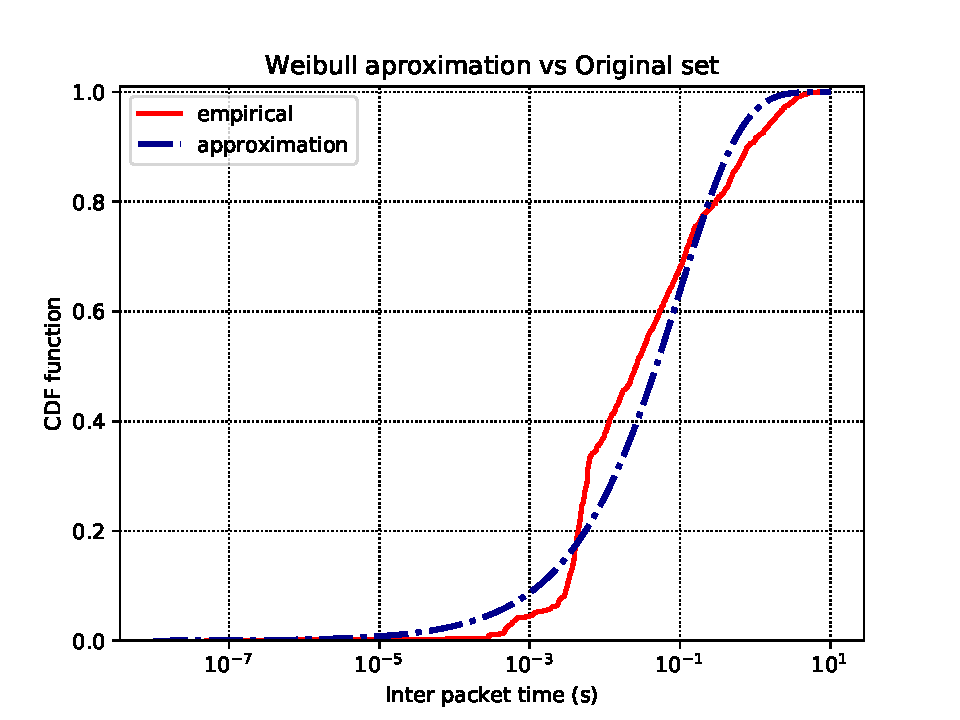
\includegraphics[width=62mm]{figures/ch4/Skype_Log_-_Weibull_aproximation_vs_Original_set}
}
\label{fig:aproximation-original-cdf}
\caption{CDF functions for the approximations of \textit{skype-pcap} inter  packet times, of many stochastic functions.}
\end{figure}

%%%%%%%%%%%%%%%%%%%%%%%
% QQplots Skype
%%%%%%%%%%%%%%%%%%%%%%%
\begin{figure}[ht!]
    \centering
    \label{fig:qq-skype}
    \subfloat[Chauchy]{
        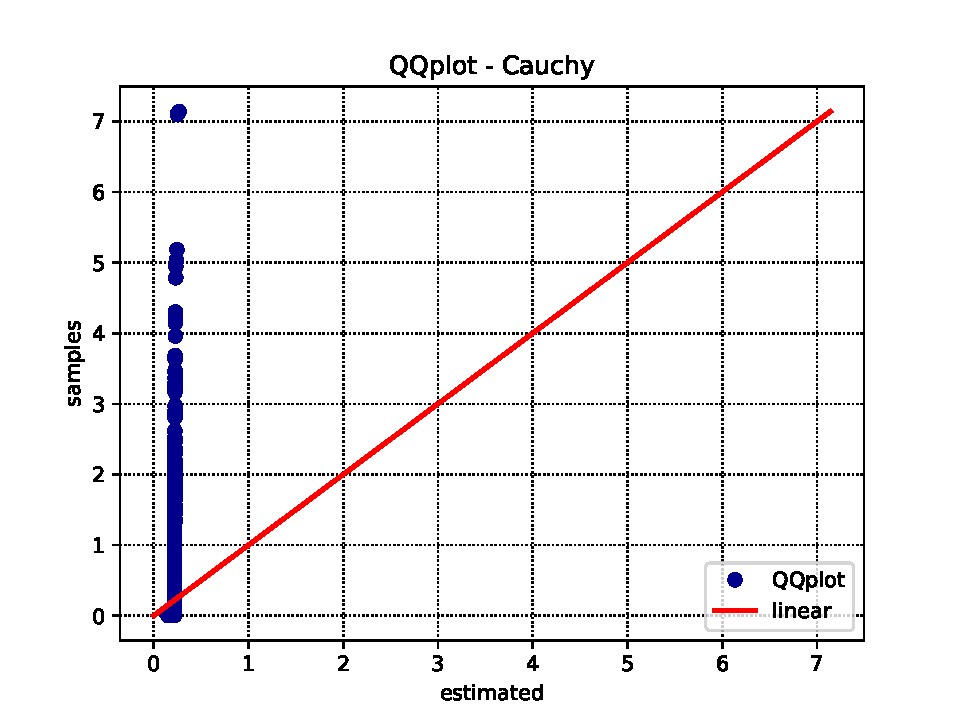
\includegraphics[width=62mm]{figures/ch4/Skype_QQplot_-_Cauchy}
    }
    \subfloat[Exponential(LR)]{
        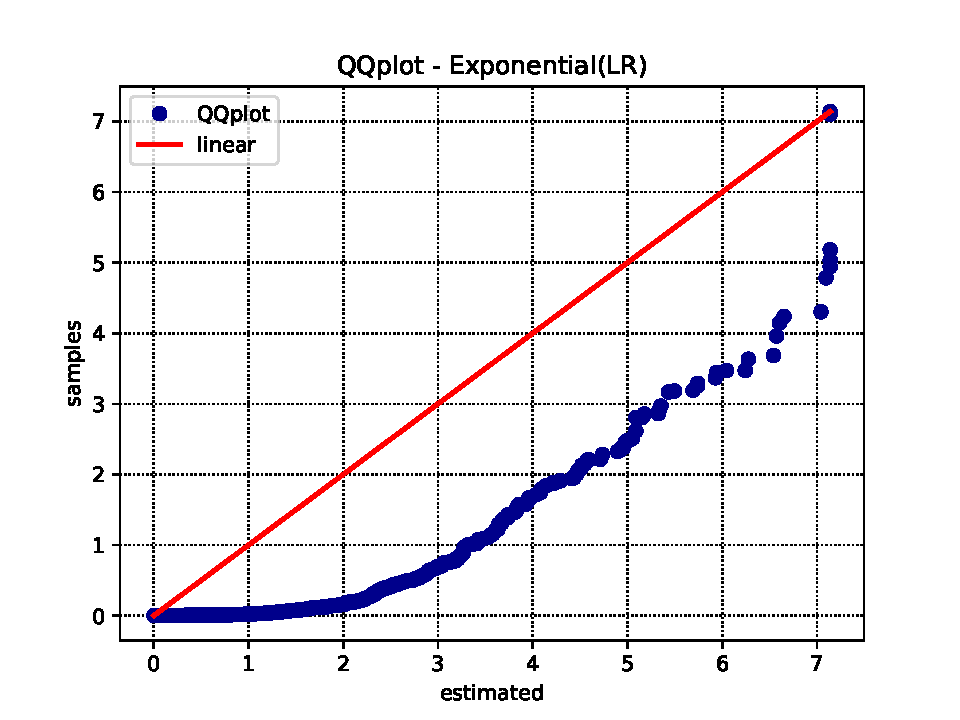
\includegraphics[width=62mm]{figures/ch4/Skype_QQplot_-_Exponential(LR)}
    }
    \hspace{0mm}
    \subfloat[Exponential(Me)]{
        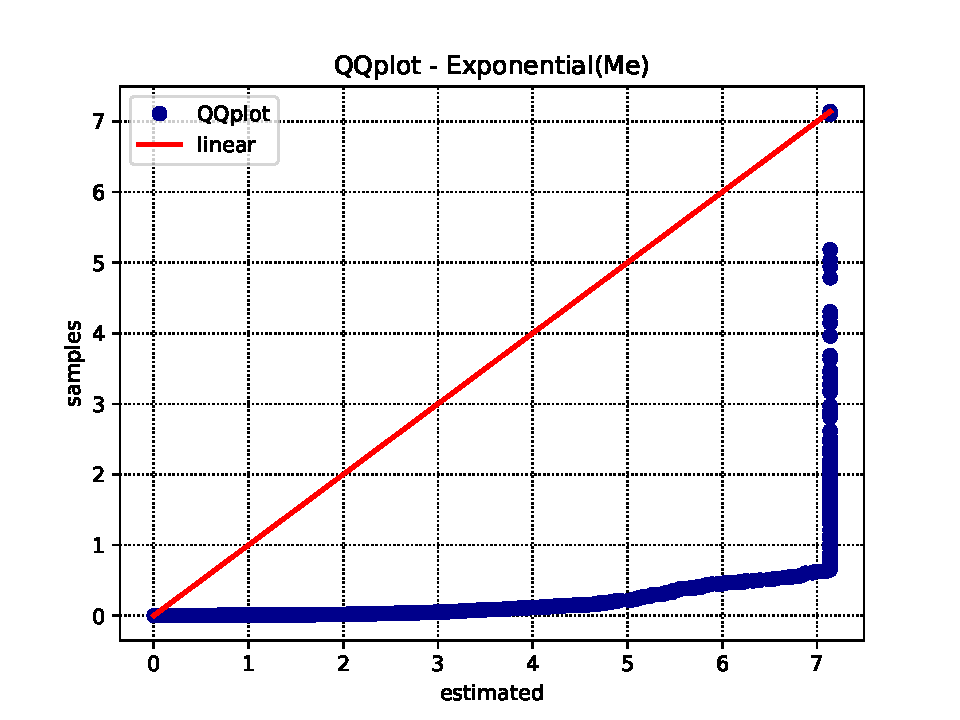
\includegraphics[width=62mm]{figures/ch4/Skype_QQplot_-_Exponential(Me)}
    }
    \subfloat[Normal]{
        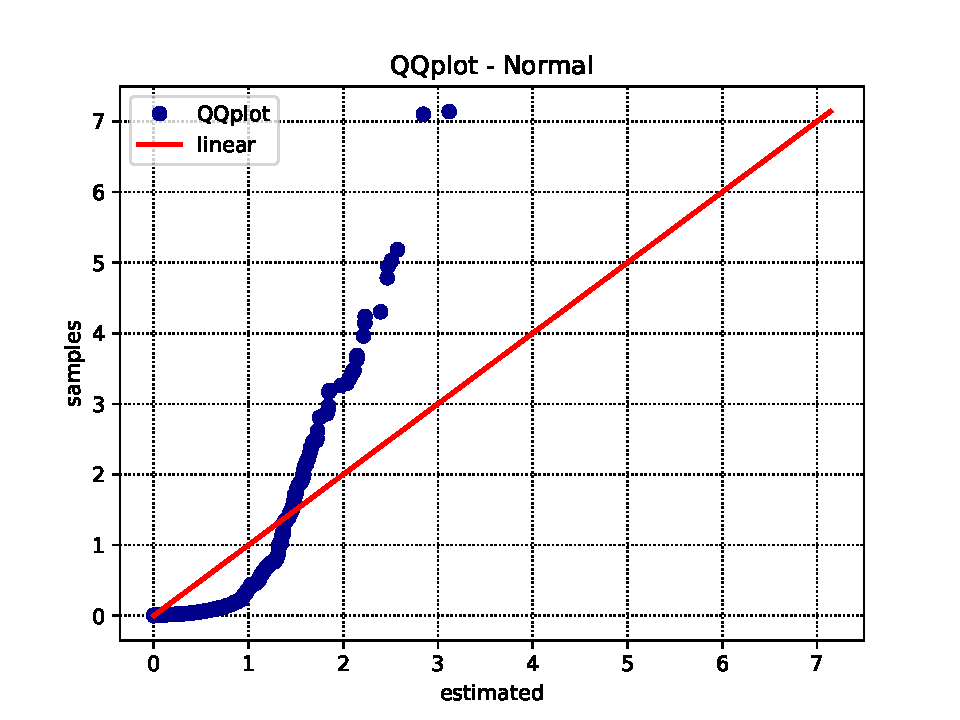
\includegraphics[width=62mm]{figures/ch4/Skype_QQplot_-_Normal}
    }
    \hspace{0mm}
    \subfloat[Pareto(LR)]{
        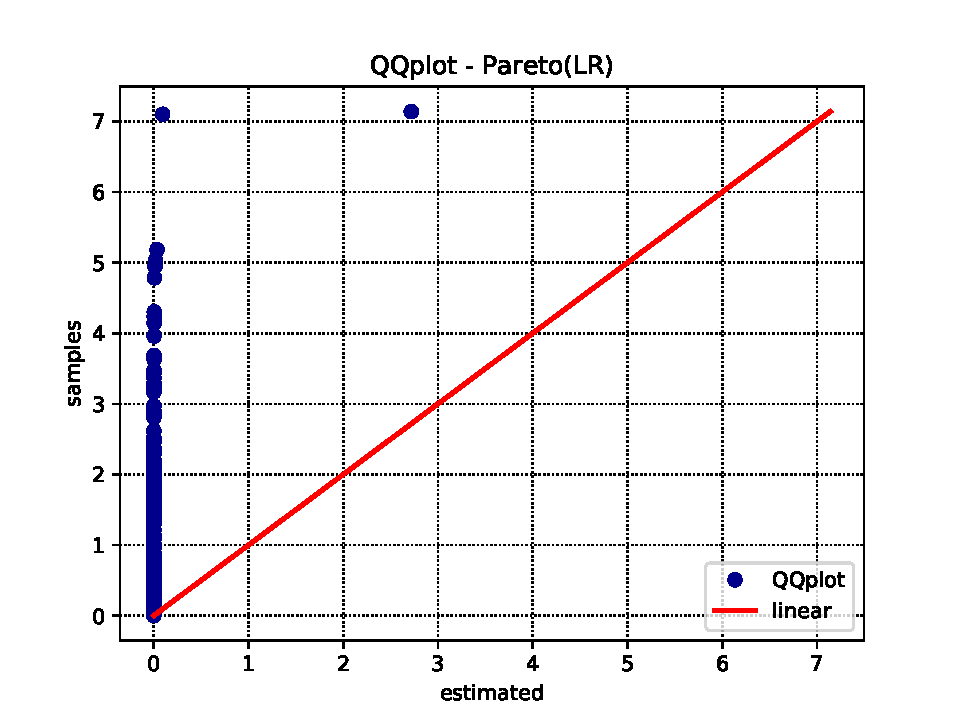
\includegraphics[width=62mm]{figures/ch4/Skype_QQplot_-_Pareto(LR)}
    }
    \subfloat[Pareto(MLH)]{
        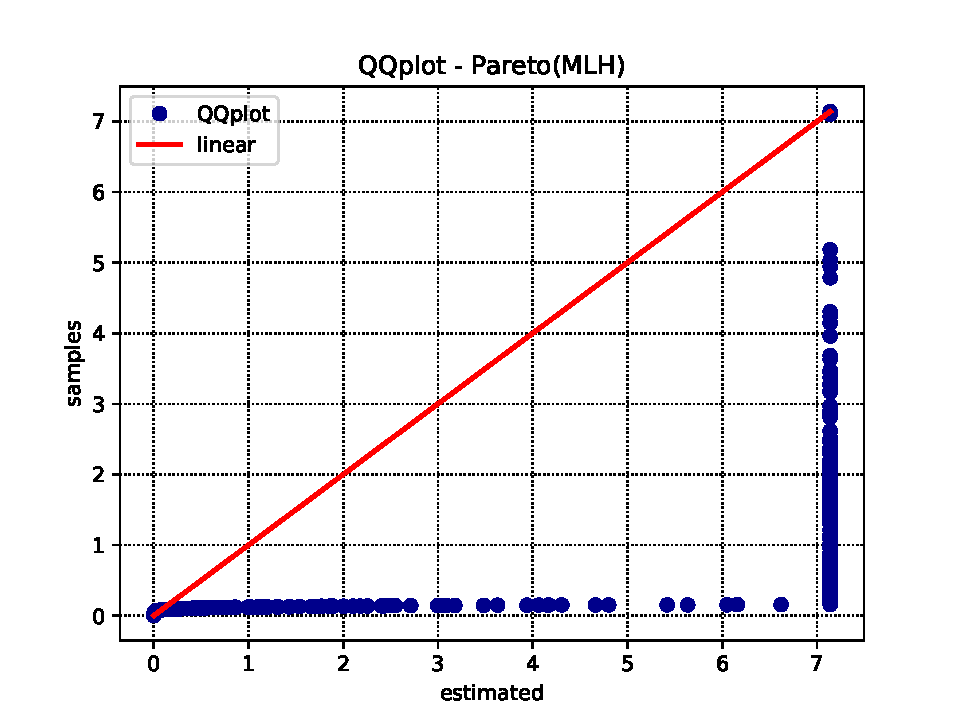
\includegraphics[width=62mm]{figures/ch4/Skype_QQplot_-_Pareto(MLH)}
    }
    \hspace{0mm}
    \subfloat[Weibull]{
        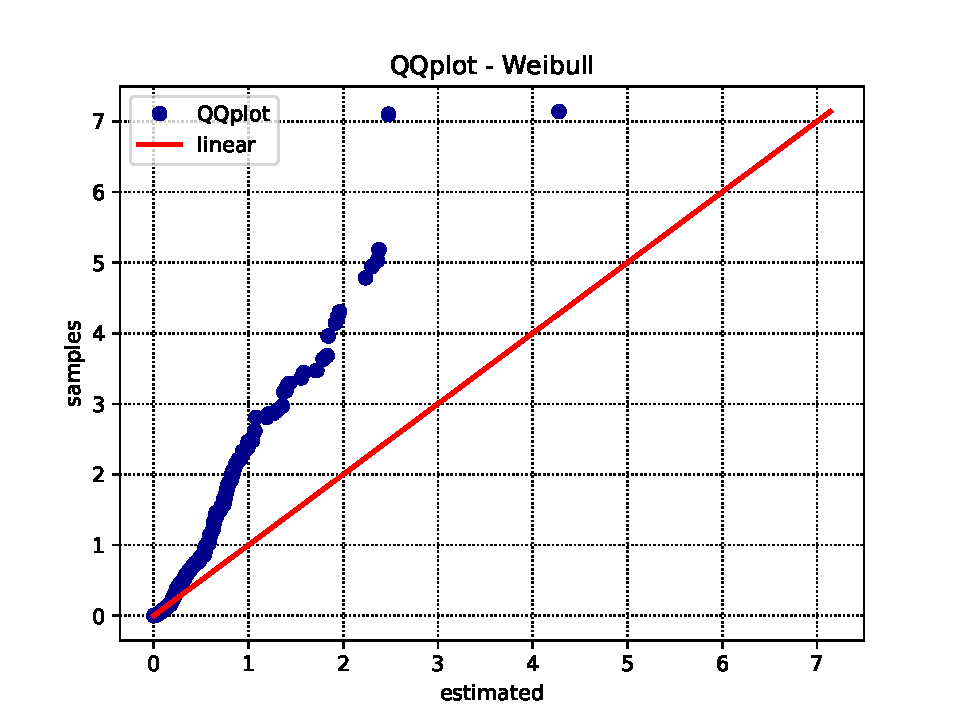
\includegraphics[width=62mm]{figures/ch4/Skype_QQplot_-_Weibull}
    }
    \caption{CDF functions for the approximations of \textit{skype-pcap} inter packet times, of many stochastic functions.}
\end{figure}

%%%%%%%%%%%%%%%%%%%%%%%
% Simulation table
%%%%%%%%%%%%%%%%%%%%%%%
\begin{sidewaystable}[!hp]
	\centering
    \caption{3 Results of the octave prototype, include BIC and AIC values, para estimated parameters for our pcap traces}
        \begin{threeparttable}[t]
        \begin{tabular}{lcccccccccc}
            \hline
            & \multicolumn{10}{c}{Trace} \\ \cline{2-11} 
            Function        & Order & AIC  & BIC  & \multicolumn{2}{c}{Parameters}  
            & Order & AIC & BIC  & \multicolumn{2}{c}{Parameters} \\ \hline 
            
            & \multicolumn{5}{c}{skype-pcap}  & \multicolumn{5}{c}{lan-diurnal-firewall-pcap}   \\ \hline 
            Cauchy          &    7 & $1.35e4$    & $2.19e4$    & $\gamma:2.75e-4$ & $x_0:2.19e-1$    
            &    5 & $-2.85e7$   & $-2.85e7$   & $\gamma:9.63e-3$ & $x_0:-3.61e-3$    \\
            Exponential(LR) &    3 & $9.69e1$   & $1.02e2$   & \multicolumn{2}{c}{$\lambda:1.51$}   
            &    6 & $1.79e6$    & $1.79e6$    & \multicolumn{2}{c}{$\lambda:8.51e-1$}    \\
            Exponential(Me) &    2 & $-4.26e2$   & $-4.28e3$   & \multicolumn{2}{c}{$\lambda:3.32$}   
            &    4 & $-3.12e7$   & $-3.12e7$   & \multicolumn{2}{c}{$ \lambda:58.78$} \\
            Normal          &    5 & $2.42e3$    & $3.31e3$    & $\mu:3.01e-1 $    & $\sigma:7.49e-1$ 
            &    7 & $Inf \tnote{1}$       & $Inf \tnote{a}$       & $\mu:1.70e-2$     & $\sigma:8.56e-2$ \\
            Pareto(LR)      &    6 & $6.4e3$   & $-8.27e3$   & $\alpha:4.14e-1$ & $x_m:5e-8$    
            &    3 & $-4.60e7$   & $-4.60e7$   & $\alpha:2.55e-1$ & $ x_m:5e-8$    \\
            Pareto(MLH)     &    4 & $3.62e2$   & $3.72e2$   & $\alpha:7.47e-2$ & $x_m:5e-8$    
            &    2 & $-5.03e7$   & $-5.03e7$   & $\alpha:1.15e-1$ & $ x_m:5e-8$    \\
            Weibull         &    1 & $-2.29e3$   & $-2.28e3$  & $\alpha:5.22e-1$ & $\beta:9.77e-2$  
            &    1 & $-5.60e7$   & $-5.60e7$   & $\alpha:3.34e-1$ & $\beta:1.83e-3$  \\ \hline    
            & \multicolumn{5}{c}{lan-gateway-pcap} & \multicolumn{5}{c}{wan-pcap}  \\ \hline
            Cauchy          &    6 & $7.14e6$    & $7.14e6$   & $\gamma:1.94e0$ &$x_0:-7.25$    
            &    7 & $5.99e7$    & $5.99e7$   & $ \gamma:8.28e2$ &$x_0:-4.52e3$    \\
            Exponential(LR) &    7 & $7.33e6$    & $7.33e6$   & \multicolumn{2}{c}{$\lambda:1.489e-1$}   
            &    6 & $5.68e7$    & $ 5.68e7$  & \multicolumn{2}{c}{$\lambda:2.2e-5$}   \\
            Exponential(Me) &    2 & $-1.09e7$   & $-1.09e7$  & \multicolumn{2}{c}{$\lambda:2.64e3$}   
            &    1 & $-6.58e7$   & $-6.58e7$  & \multicolumn{2}{c}{$\lambda:6.58e5$} \\
            Normal          &    5 & $-9.35e6$   & $-9.35e6$  & $\mu:3.79e-4$   &$\sigma:6.60e-4$ 
            &    2 & $-6.39e7$   & $-6.39e7$  & $\mu:2e-6$     & $\sigma:1e-6$ \\
            Pareto(LR)      &    4 & $-1.02e7$   & $-1.02e7$  & $\alpha:1.489e-1 $ & $x_m:5e-8 $    
            &    4 & $-5.31e7$   & $-5.31e7$  & $\alpha:4e-14\tnote{b}$ & $x_m:5e-8 $    \\
            Pareto(MLH)     &    3 & $-1.03e7$   & $-1.03e7$  & $\alpha:1.362e-1$ & $x_m:5e-8 $    
            &    5 & $-6.25e7$   & $-6.25e7$  & $\alpha:3.39e-1$ & $x_m:5e-8 $    \\
            Weibull         &    1 & $-1.10e7$   & $-1.10e7$  & $\alpha:2.81e-1$ & $\beta:5.54e-4$  
            &    3 & $-5.46e7$   & $-5.46e7$  & $\alpha:7.64e-2$ & $\beta:1e-6$  \\ \hline
        \end{tabular}
            \begin{tablenotes}
            \item[1] The computation of the likelihood function has exceeded the computational precision used, so it was the highest AIC and BIC  for this trace.
            \item[2] The linear regression did not converge to a valid value, so we used a small value("infinitesimal") instead to perform the computations.
            \end{tablenotes}
        \end{threeparttable}
    \label{tab:prototype-results}
\end{sidewaystable}

%%%%%%%%%%%%%%%%%%%%%%%
% AIC BIC  diff
%%%%%%%%%%%%%%%%%%%%%%%
\begin{table}[]
\centering
\caption{Relative difference between $AIC$ and $BIC$.}
\begin{tabular}{ccccc}
\hline
& skype-pcap  & \begin{tabular}[c]{@{}c@{}}lan-gateway-\\ pcap\end{tabular} & wan-pcap    & \begin{tabular}[c]{@{}c@{}}lan-diurnal-\\ firewall-pcap\end{tabular} \\ \hline
Weibull         & -0.434838\% & -0.000211\%                                                 & -0.000048\% & -0.000047\%                                                          \\
Normal          & 0.409772\%  & -0.000248\%                                                 & -           & -0.000041\%                                                          \\
Exponential(LR) & 5.006892\%  & 0.000158\%                                                  & 0.000753\%  & 0.000022\%                                                           \\
Exponential(Me) & -1.174737\% & -0.000106\%                                                 & -0.000043\% & -0.000019\%                                                          \\
Pareto(LR)      & 0.155122\%  & -0.000226\%                                                 & -0.000058\% & 0.000028\%                                                           \\
Pareto(MLH)     & 2.712815\%  & -0.000226\%                                                 & -0.000053\% & -0.000041\%                                                          \\
Cauchy          & 0.073890\%  & 0.000324\%                                                  & -0.000094\% & 0.000043\%                                                           \\ \hline
\end{tabular}
\label{tab:aic-bic-diff}
\end{table}

%%%%%%%%%%%%%%%%%%%%%%%
% Skype  - Correlation, Hurst, Mean Standard Deviation
%%%%%%%%%%%%%%%%%%%%%%%
\begin{figure}[ht]
    \centering
    \subfloat[Correlation]{
        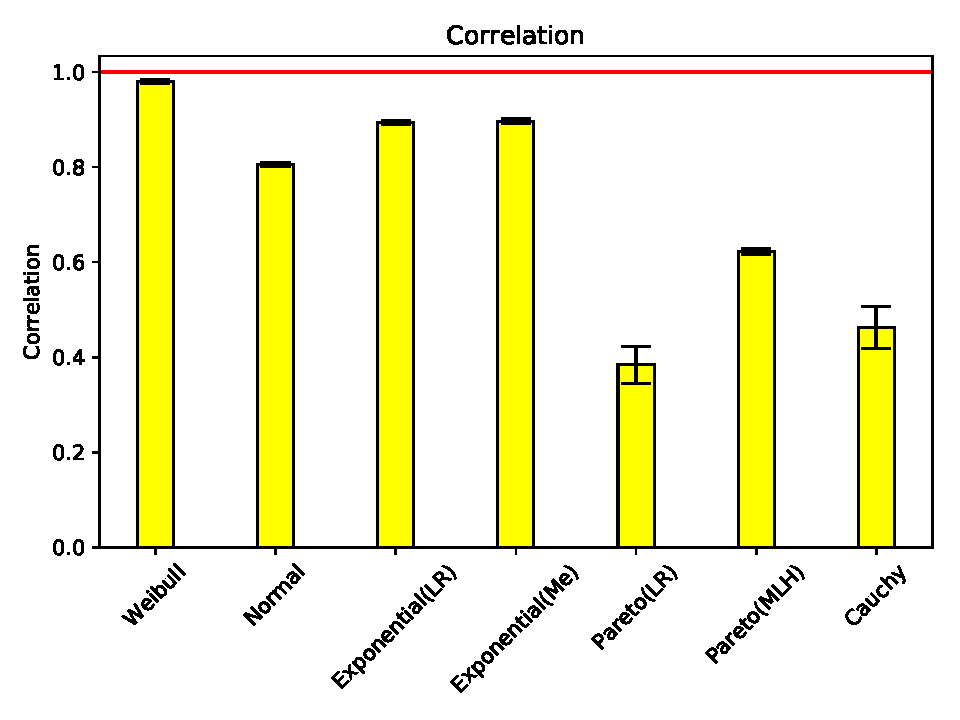
\includegraphics[width=62mm]{figures/ch4/Skype_Correlation}
        \label{correlation-skype}
    }
    \hspace{0mm}
    \subfloat[Hust Exponent]{
        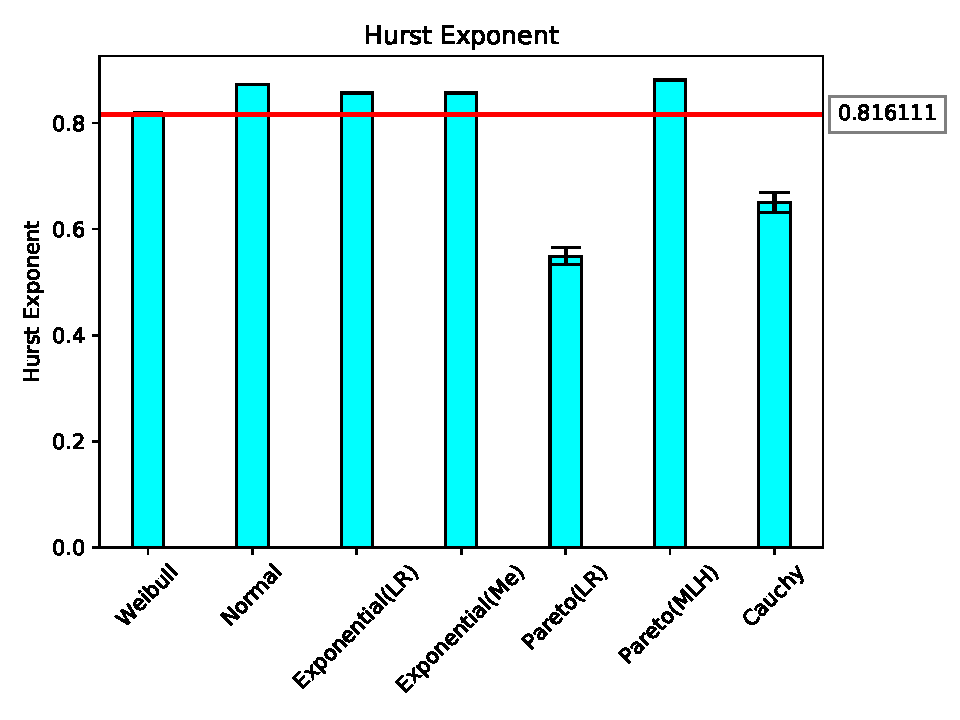
\includegraphics[width=62mm]{figures/ch4/Skype_Hurst_Exponent}
        \label{hurst-skype}
    }
    \hspace{0mm}
    \subfloat[Mean]{
        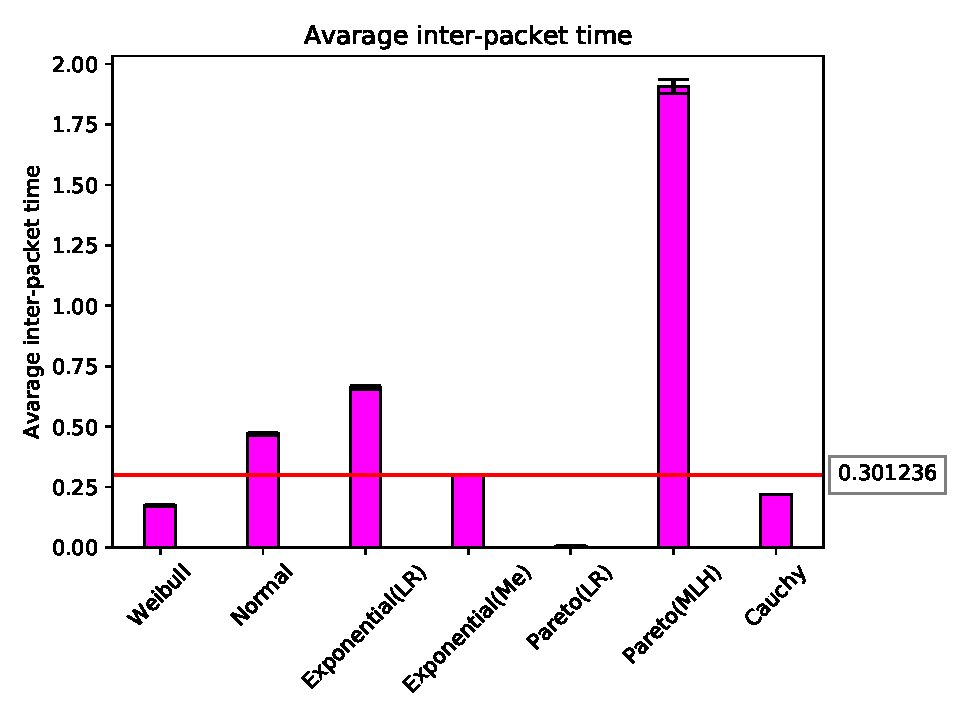
\includegraphics[width=62mm]{figures/ch4/Skype_Mean}
        \label{mean-skype}
    }
    \hspace{0mm}
    \subfloat[Standard Deviation]{
        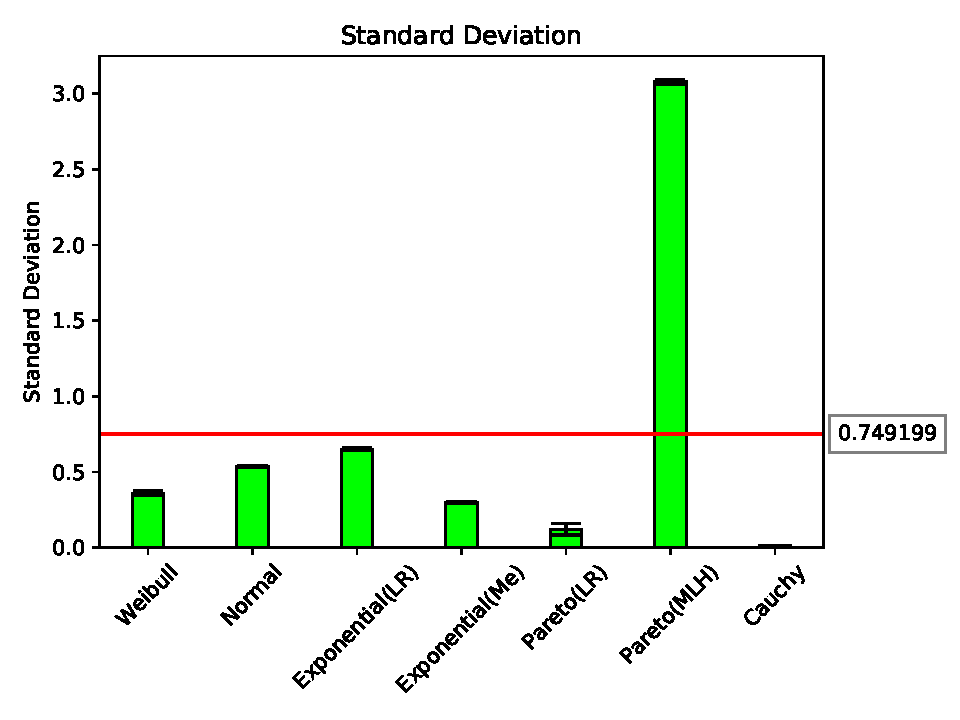
\includegraphics[width=62mm]{figures/ch4/Skype_Standard_Deviation}
        \label{std-skype}
    }
    \caption{Statistical parameters of \textit{skype-pcap} and its approximations}
    \label{fig:correlation-hurst-skype-pcap}
\end{figure}
%%%%%%%%%%%%%%%%%%%%%%%
% bigFlows -  Correlation, Hurst, Mean Standard Deviation
%%%%%%%%%%%%%%%%%%%%%%%
\begin{figure}[ht]
    \centering
    \subfloat[Correlation]{
        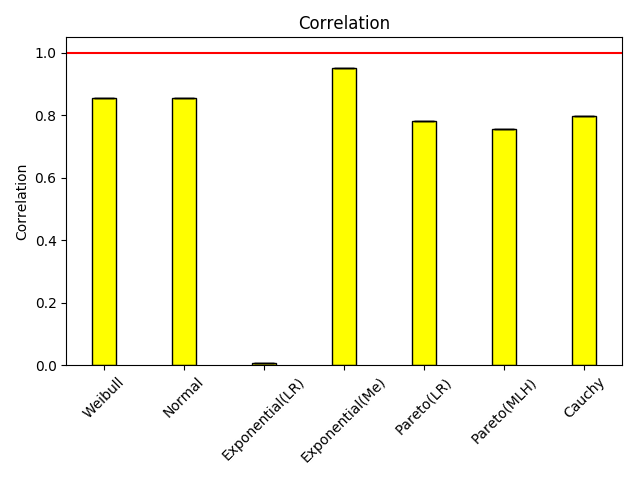
\includegraphics[width=62mm]{figures/ch4/bigFlows_Correlation}
        \label{bigFlows-correlation-skype}
    }
    \hspace{0mm}
    \subfloat[Hust Exponent]{
        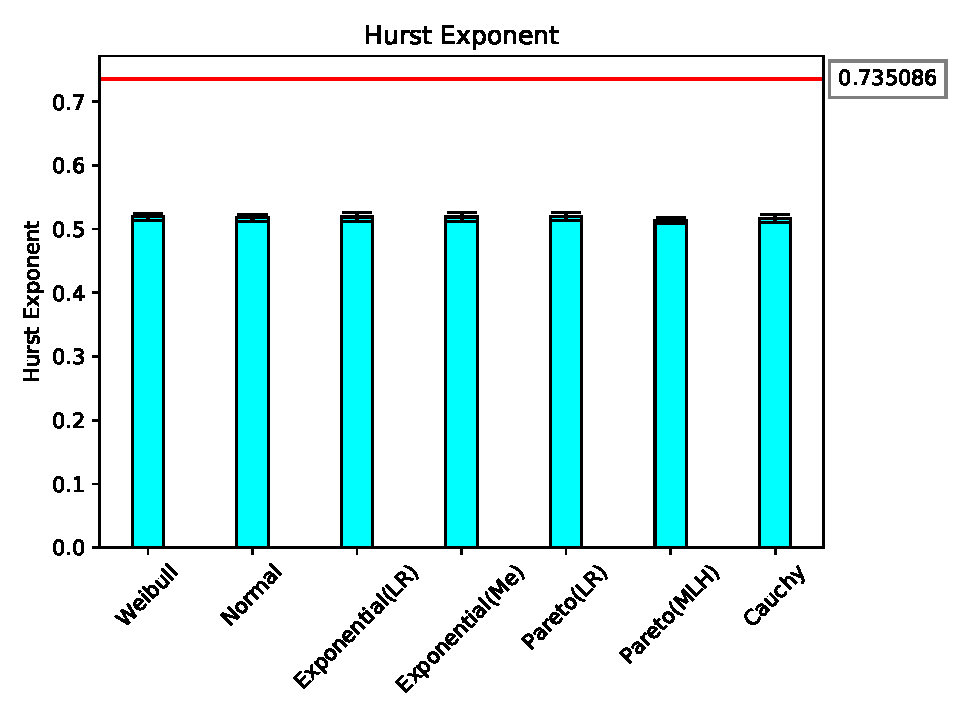
\includegraphics[width=62mm]{figures/ch4/bigFlows_Hurst_Exponent}
        \label{bigFlows-hurst-skype}
    }
    \hspace{0mm}
    \subfloat[Mean]{
        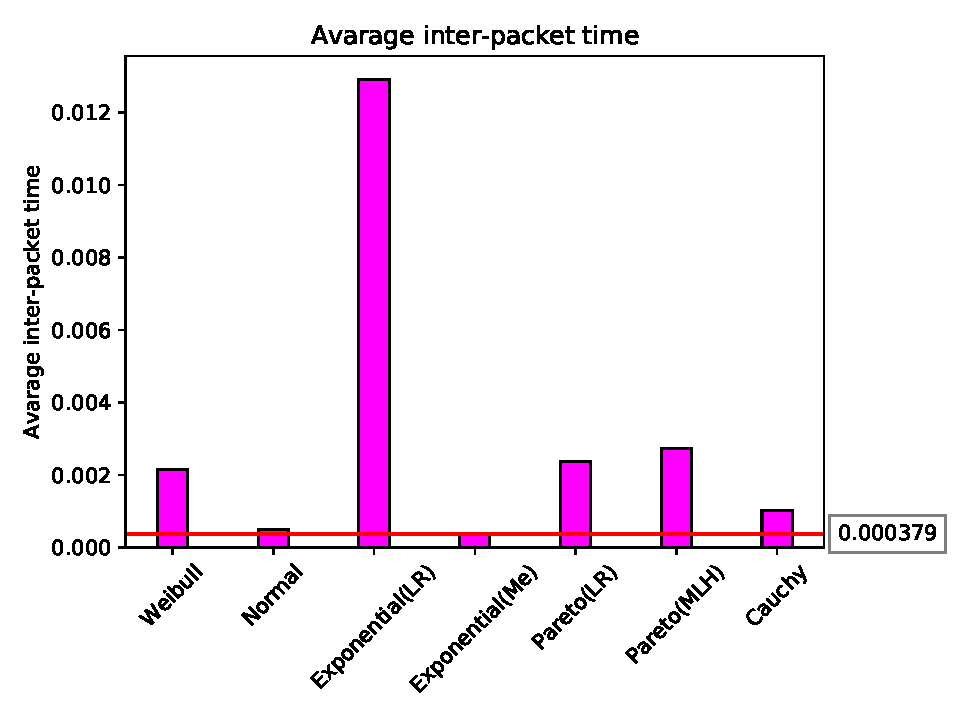
\includegraphics[width=62mm]{figures/ch4/bigFlows_Mean}
        \label{bigFlows-mean-skype}
    }
    \hspace{0mm}
    \subfloat[Standard Deviation]{
        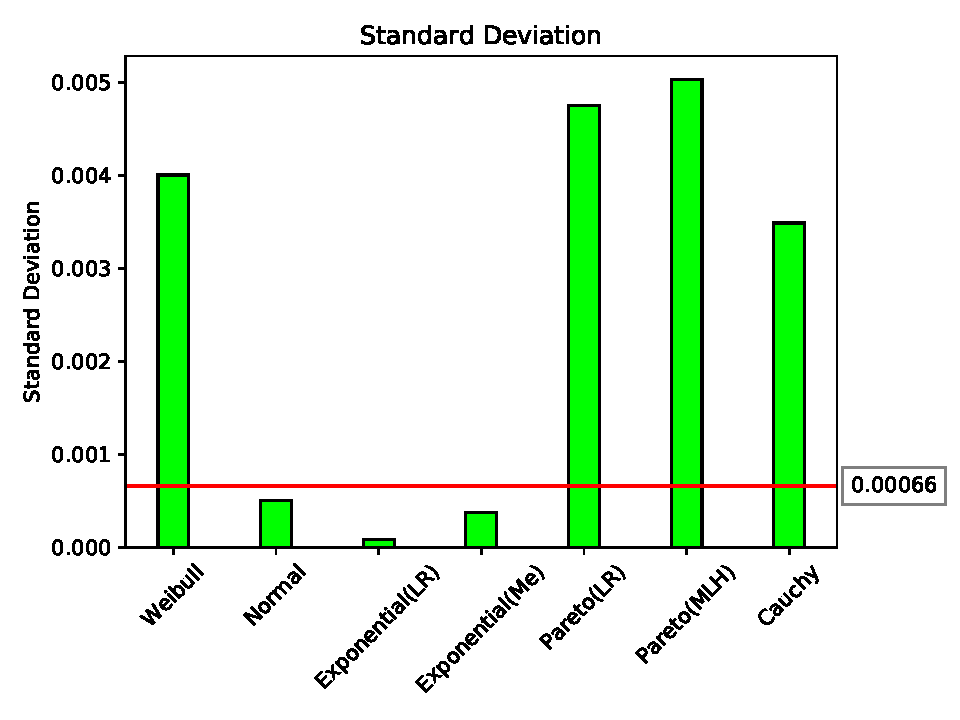
\includegraphics[width=62mm]{figures/ch4/bigFlows_Standard_Deviation}
        \label{bigFlows-std-skype}
    }
    \caption{Statistical parameters of \textit{lan-gateway-pcap} and its approximations}
    \label{fig:correlation-hurst-lan-gateway-pcap}
\end{figure}

%%%%%%%%%%%%%%%%%%%%%%%
% lanDirunal  - correlation, Hurst, Mean Standard Deviation
%%%%%%%%%%%%%%%%%%%%%%%
\begin{figure}[]
    \centering
    \subfloat[Correlation]{
        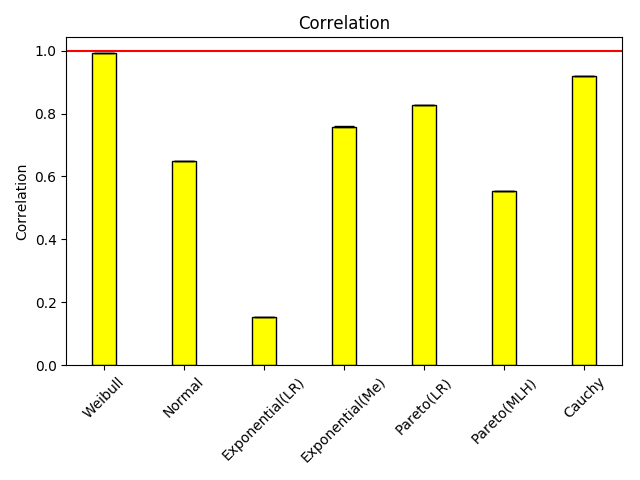
\includegraphics[width=62mm]{figures/ch4/Lan_Correlation}
        \label{Lan-correlation-skype}
    }
    \hspace{0mm}
    \subfloat[Hust Exponent]{
        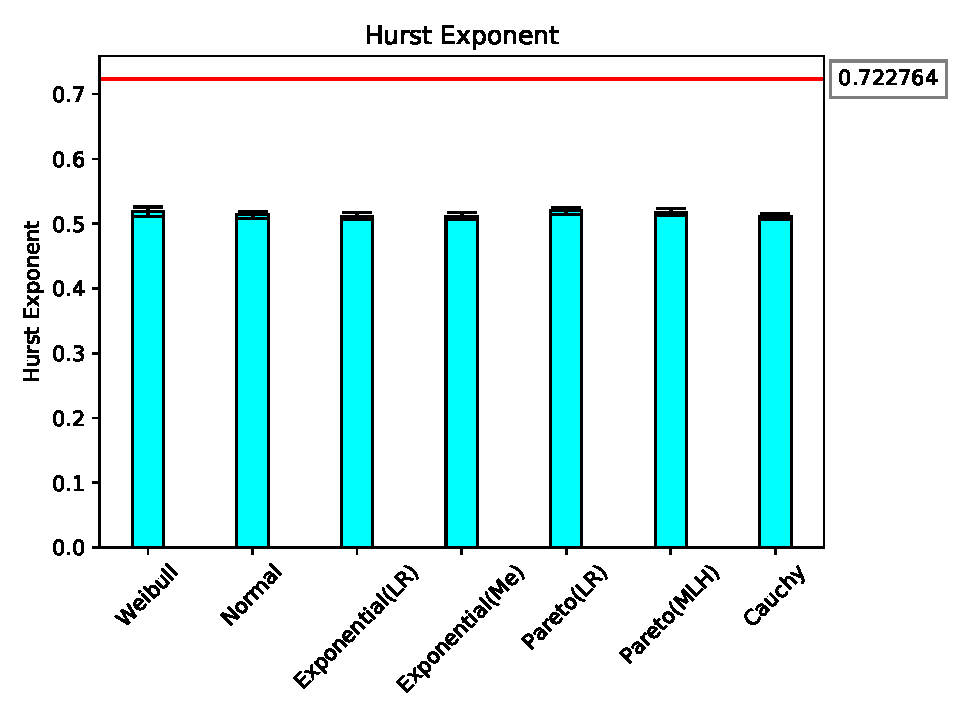
\includegraphics[width=62mm]{figures/ch4/Lan_Hurst_Exponent}
        \label{Lan-hurst-skype}
    }
    \hspace{0mm}
    \subfloat[Mean]{
        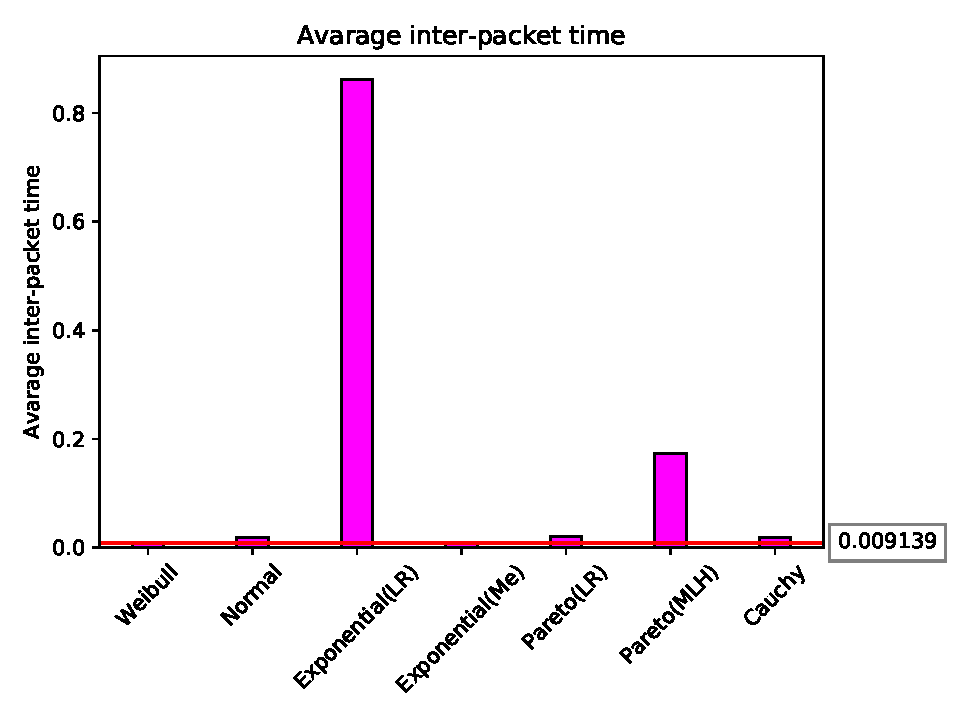
\includegraphics[width=62mm]{figures/ch4/Lan_Mean}
        \label{Lan-mean-skype}
    }
    \hspace{0mm}
    \subfloat[Standard Deviation]{
        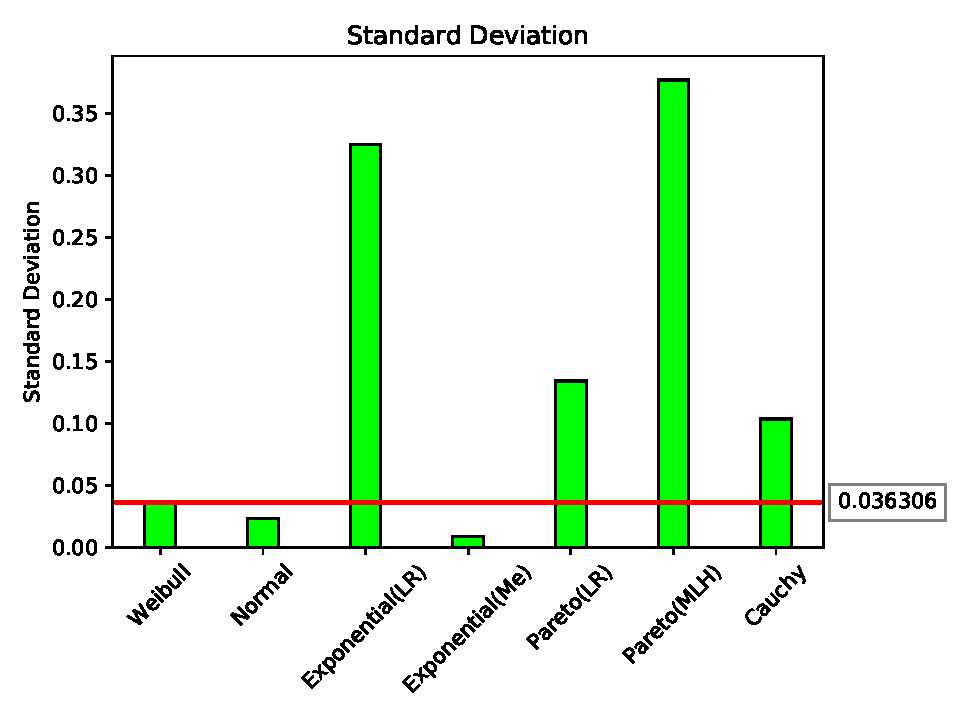
\includegraphics[width=62mm]{figures/ch4/Lan_Standard_Deviation}
        \label{Lan-std-skype}
    }
    \caption{Statistical parameters of \textit{Lan-pcap} and its approximations}
    \label{fig:correlation-hurst-Lan-pcap}
\end{figure}

%%%%%%%%%%%%%%%%%%%%%%%
% Wan - correlation, Hurst, Mean Standard Deviation
%%%%%%%%%%%%%%%%%%%%%%%
\begin{figure}[]
    \centering
    \subfloat[Correlation]{
        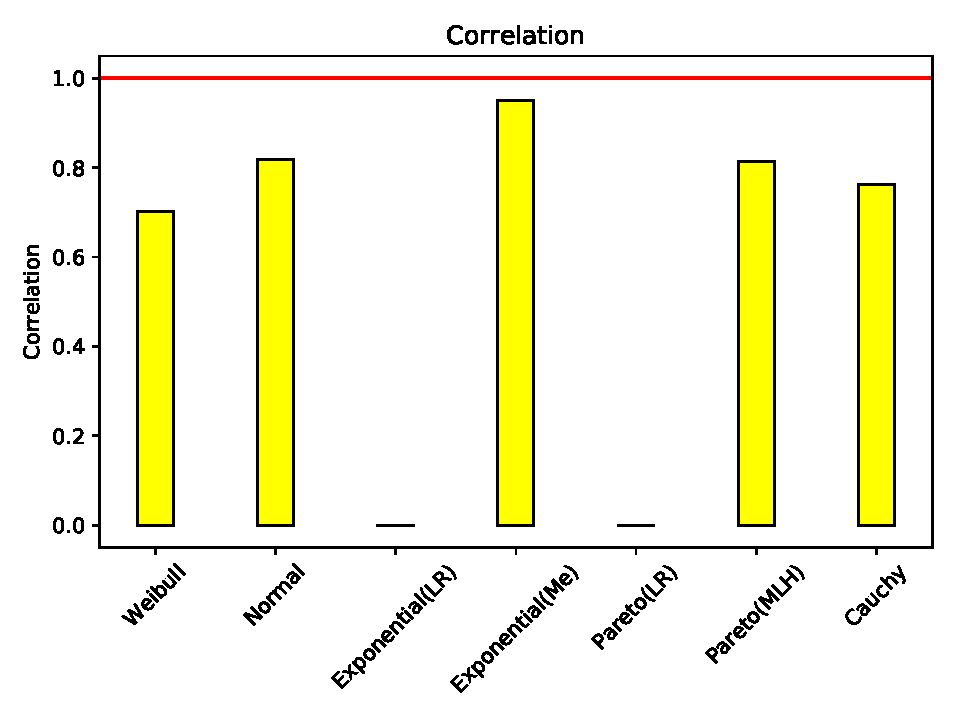
\includegraphics[width=62mm]{figures/ch4/Wan_Correlation}
        \label{Wan-correlation-skype}
    }
    \hspace{0mm}
    \subfloat[Hust Exponent]{
        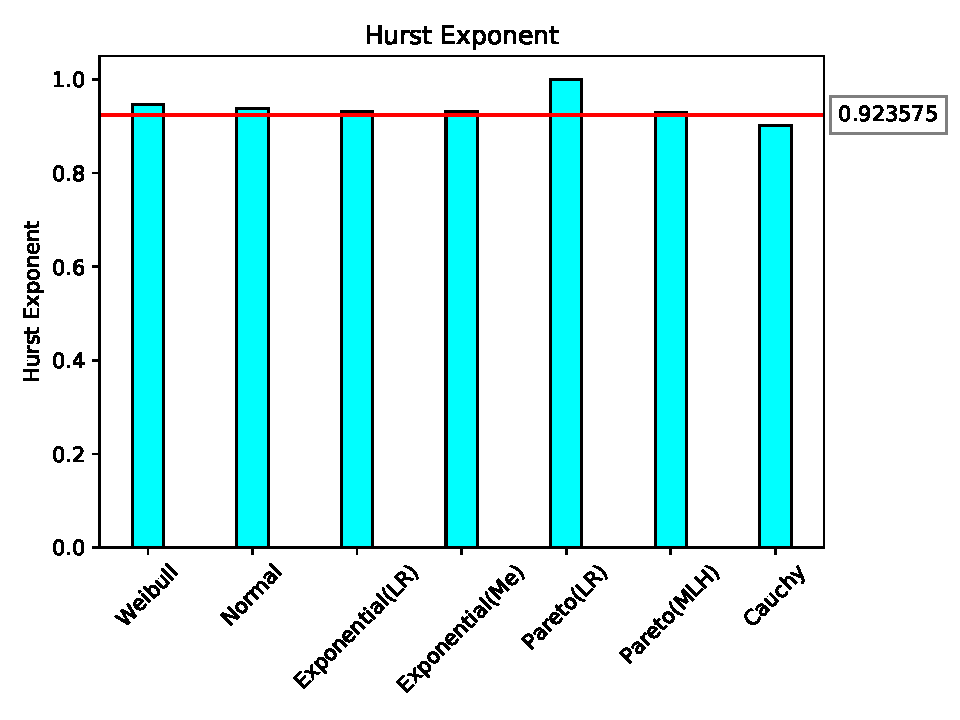
\includegraphics[width=62mm]{figures/ch4/Wan_Hurst_Exponent}
        \label{Wan-hurst-skype}
    }
    \hspace{0mm}
    \subfloat[Mean]{
        \includegraphics[width=62mm]{figures/ch4/Wan_Mean}
        \label{Wan-mean-skype}
    }
    \hspace{0mm}
    \subfloat[Standard Deviation]{
        \includegraphics[width=62mm]{figures/ch4/Wan_Standard_Deviation}
        \label{Wan-std-skype}
    }
    \caption{Statistical parameters of \textit{wan-pcap} and its approximations}
    \label{fig:correlation-hurst-wan-pcap}
\end{figure}

%%%%%%%%%%%%%%%%%%%%%%%
%validation Cost function
%%%%%%%%%%%%%%%%%%%%%%%
\begin{figure}[t!]
    \centering
    \subfloat[\textit{skype-pcap}]{
        \includegraphics[width=62mm]{figures/ch4/Skype_costFunction}
        \label{cost-skype-pcap}
    }
    \hspace{0mm}
    \subfloat[\textit{lan-gateway-pcap}]{
        \includegraphics[width=62mm]{figures/ch4/bigFlows_costFunction}
        \label{cost-lan-gateway-pcap}
    }
    \hspace{0mm}
    \subfloat[\textit{lan-firewall-diurnal-pcap}]{
        \includegraphics[width=62mm]{figures/ch4/Lan_costFunction}
        \label{cost-lan-pcap}
    }
    \hspace{0mm}
    \subfloat[\textit{wan-pcap}]{
        \includegraphics[width=62mm]{figures/ch4/Wan_costFunction}
        \label{cost-wan-pcap}
    }
    \caption{Cost function for each one of the datasets used in this validation process}
    \label{fig:cost-function}
\end{figure}

%%%%%%%%%%%%%%%%%%%%%%%
%validation Cost function
%%%%%%%%%%%%%%%%%%%%%%%
%\begin{figure}[t!]
%    \centering
%    \includegraphics[width=100mm]{figures/ch4/aic-bic_vs_costFunction_order}
%    \caption{Comparison of model selection order com cost function and AIC/BIC}
%    \label{fig:cost-function_vs_aic-bic}
%\end{figure}

\begin{figure}[!ht]
	\centering
	\includegraphics[scale=1]{figures/ch4/aic-bic-order}
	\caption{Comparision of the quality order of each model given by AIC and BIC}
	\label{fig:aic-bic-order}
\end{figure}


\begin{figure}[ht!]
\includegraphics[scale=1]{figures/ch4/cost-function-summary}
\caption{Cost function for each one of the datasets used in this validation process.}
\label{fig:model-order-cost}
\end{figure}

\begin{figure}[ht!]
\includegraphics[scale=1]{figures/ch4/aicbic-costfunction-relative-diff}
\caption{Comparison of the model selection order for $BIC$/$AIC$ and the cost function $J$ for each \textit{pcap}.}
\label{fig:cost-function_vs_aic-bic}
\end{figure}



\begin{algorithm}[ht!]
    \caption{stochasticModelFitting}
    \label{alg:stochasticModelFitting}
    \begin{algorithmic}[1]
        \small        \Function{stochasticModelFitting}{$interArrivalData, criterion$}
        \State $m = interArrivalData.size$
        \State $interArrivalData = interArrivalData + MIN\_TIME$
        \If{$m < MINIMUM\_AMOUNT\_OF\_PACKETS$}
        \State $model\_list = \{constant\}$
        \Else
        \State $model\_list = \{weibull, pareto\_lr, pareto\_mlh, exponential\_me, exponential\_lr, normal,$
        \State $cauchy, constant\}$
        \EndIf
        
        \For{$model$ \textbf{in} $model\_list$}
        \State $model.fitting\_model(interArrivalData)$
        \EndFor
        \State $model\_list.sort(criterion)$
        \State \textbf{return} $model\_list$
        \EndFunction
    \end{algorithmic}
\end{algorithm}

Here in this chapter we only discuss the plots achieved obtained by the \textit{pcap} \textit{skype-pcap} for simplicity. The other plots are provided and commented on the appendix ~\ref{ap:aditional-plots}. In the figure~\ref{fig:aproximation-original-cdf} we present all estimated CDF functions along with the empirical CDF, for the trace \textit{skype-pcap}. They are on log-scale, which provide a better visualization for small time scales. In the case of the normal function, all values smaller than zero were set to zero on the plot. Is possible to see different accuracies and types of fittings on each plot. Visually, the best fit seems to be the Weibull trough linear regression. 

Analyzing the plots, and what they would mean, our Cauchy fitting would impose almost constant traffic, with the inter-packet time close to the mean. On the trace \textit{skype-pcap} the exponential plots seems not to represent well the small values of inter-packet times. This is due fact that an exponential process is good at describing values close to the average. But, it fails to represent values too small and higher. On the other hand, a self-similar process like Weibull and Pareto are better serving inter-packet times with higher dispersion. Pareto(MLH) has a slow convergence, which means this distribution may generate values of inter-packet times too large. 

Analyzing the QQplots, we can observe that in most of the distribution, the samples (original data) has a much havier-tail effect than in the estimated data. We can verify this by the by the almost blue horizontal lines formed by the x-marks. But, the Weibull distribution follows much closer the original data. Also is possible to see that the sample has a right skew compared to the estimation on Exponential(LR), Exponential(Me), Normal, and Pareto(MLH). This "right-skew" means that this estimation would not represent so well small values of time in this case. On the other hand, Pareto(LR) and Weibull would not suffer from this problem.

The results for the AIC, BIC, and parameters of all four traces are at the table~\ref{tab:prototype-results}.  The results for \textit{wan-pcap} and \textit{lan-firewall-diurnal-pcap} are on the table ~\ref{tab:prototype-results}. The differences between BIC and AIC values from a same stochastic function all cases are small compared to the difference between their values calculated between different distributions. Since we compared many different types of Ethernet traces, this result indicates that for inter-packet times, use AIC or BIC as decision criteria should not influence the results from most of the cases. 

On our previsions, Weibull and Pareto(MLH and LR) are the best options. We expected that since both are heavy-tailed functions. But Cauchy on most of the tests, even being a heavy-tailed distribution, seems to no present a proper fitting. The quick divergence of the tangent function is the cause for this lousy fitting.

Analyzing the quality of AIC and BIC as criteria of choose on \textit{skype-pcap}, based on the results form figure ~\ref{fig:correlation-hurst-skype-pcap} we see that concerning Correlation and Self-similarity it picked the right model: Weibull. Also regarding average packet rate and dispersion, it is still one of the best choices (along with Exponential(Me), Pareto(LR) and Cauchy). The third and the fourth choices (Pareto(LR)) and Exponential(LR) also are good options in most of these metrics. But, Pareto(MLH) is presented as the second best choice, and it had poor results in comparison to the others, especially on mean, correlation and dispersion. 

All these results are abstracted by the cost function $J$. As we can see, on all pcaps, the best function selected by BIC and AIC(table~\ref{tab:prototype-results}) also had the small cost(figure~\ref{fig:cost-function}). 

Another important observation is the fact that exponential function was able to provide the best fitting for the \textit{wan-pcap}. The reasons for this behavior are both results of a much great traffic with no long-range gaps, and the precision of the measurement.


Since there is a lot of information on table~\ref{tab:prototype-results} and on the figure~\ref{fig:cost-function}, we capture just the order of choise form each \textit{pcap} plotted on the figure~\ref{fig:cost-function_vs_aic-bic}. We can see that expecially on the best fittings, the results were closer. Just for the \textit{lan-gateway-pcap} the results from the best and second best models were flipped. On all the other cases, the choises were the same. For the worsts models, the results tend to differ more, and loose correlation. It is not a bad thing, since they were not good choices after all. 



\subsection{Conclusion}


We can conclude that using AIC or BIC as criteria for choosing good models for inter-packet times is a good choice.

Except by the Pareto function modeled using the Maximum likelihood method, have comparative results between the simulations and the AIC/BIC goes. The best fittings according to the AIC/BIC usually returned very accurate models, with a small error between the mean and fractal level, and correlation close to one. The models selected as the worsts traditionally yielded poor results.

It is important to notice that in some cases, some stochastic functions may perform poorly, and in other provide an accurate fitting, what justify the application of the criteria in all new experiments. For example, Weibull usually plays pretty well, but in some cases, perform poorly, or may even diverge. 

We do not rely on only one type of parameterization. This approach turns our methodology more robust, since a linear regression may diverge. But always there will be a peaceable model, since our estimations for Normal, Exponential (Me) and Pareto (MLH) cannot. Models which the linear regression diverges will have very high and positive BIC/AIC estimations, and will not stand as primary options.


\section{ON/OFF Periods and Application classification}

    
\begin{algorithm}[ht!]
    \caption{calcOnOff}
    \label{alg:calcOnOff}
    \begin{algorithmic}[1]
        \small
        \Function{calcOnOff}{$arrivalTime, deltaTime, cutTime, minOnTime$}%\Comment{Where A - array, p - left, q - middle, r - right}
        \State $m = deltaTime.length() - 1$
        \State $j = 0$
        \State $lastOff = 0$
        \State $pktCounterSum = 0$
        \State $fileSizeSum = 0$
        \For{$i = 0:m$}
        \State $pktCounterSum = pktCounterSum + 1$
        \State $fileSizeSum = fileSizeSum + psSizeList[i, 1]$
        \If{$deltaTime[i] > cutTime$} 
        \If{$i == 1$} \Comment{if the first is session-off time}
        \State $j++$
        \State $onTimes.push(minOnTime)$
        \State $offTimes.push(deltaTime[i])$
        \State $pktCounter.push(pktCounterSum)$
        \State $fileSize.push(fileSizeSum)$
        \State $pktCounterSum = 0$
        \State $fileSizeSum = 0$
        \Else \Comment{base case} 
        \State $pktCounter.push(pktCounterSum)$
        \State $fileSize.push(fileSizeSum)$
        \State $pktCounterSum = 0$
        \State $fileSizeSum = 0$
        \If{$j == 0$}
        \State $onTimes.push(arrivalTime[i - 1])$
        \State $offTimes.push(deltaTime[i])$
        \Else \Comment{others on times} 
        \State  $onTimes.push(max(deltaTime[i-1] - deltaTime[lastOff], minOnTime))$ 
        \State  $offTimes.push(deltaTime[i])$
        \EndIf
        \State $lastOff = i$
        \EndIf 
        \EndIf       
        \EndFor
        \State $pktCounterSum = pktCounterSum + 1$
        \State $fileSizeSum = fileSizeSum + psSizeList[m]$
        \If{$lastOff == m - 1$} \Comment{ if last is session-off }
        \State $onTimes.push(minOnTime)$ % on time
        \Else \Comment{ base last case}
        \If{$lastOff \neq 0$}
        \State $onTimes.push(arrivalTime[m] - arrivalTime[lastOff])$ 
        \Else 
        \State $onTimes.push(arrivalTime[m])$ \Comment{there was just on time}
        \EndIf
        \EndIf
        \State $pktCounter.push(pktCounterSum)$
        \State $fileSize.push(fileSizeSum)$
        \State \textbf{return} $onTimes, offTimes, pktCounter, fileSize$
        \EndFunction
    \end{algorithmic}
\end{algorithm}
    
\begin{table}[ht!]
    \centering
    \caption{Application match table}
    \label{tab:application-protocols}
    \begin{tabular}{lll}
        \hline
        Application Protocol & Transport Protocols & Transport Ports \\ \hline
        HTTPS               & TCP                & 443             \\
        FTP                 & TCP                & 20, 21          \\
        HTTP                & TCP                & 80              \\
        BGP                 & TCP                & 179             \\
        DHCP                & UDP                & 67, 68          \\
        SNMP                & UDP, TCP           & 161             \\
        DNS                 & UDP, TCP           & 53              \\
        SSH                 & UDP, TCP           & 22              \\
        Telnet              & UDP, TCP           & 23              \\
        TACACS              & UDP, TCP           & 49              \\ \hline
    \end{tabular}
\end{table}




In this section, we briefly show another method used by the \textit{TraceAnalyzer} component. The first to calculate the session ON and OFF times. The second classify applications based on its transport protocol and ports. In the table ~\ref{tab:methods} we summarize the stack of models used to create the Compact Trace Descriptor (CTD file). 



We developed an algorithm to calculate the times between the ON and OFF times of the \textit{files}, and the number of packets and bytes as well. It uses a list of packet arrival times(relative to the first), the time between packets and packet sizes. It defines a minimum time of ON acceptable. These times are used for two reasons:

\begin{itemize}
\item In case of a \textit{file} of just one packet, it will not produce an ON-time of zero
\item It avoids a \textit{file} On time too small, which may be less than acceptable for packet generator tools.
\end{itemize}

As explained in the previous chapter, a \textit{file} is defined by a large OFF time, we call $cutTime$. If an inter-packet $deltaTime$ time is larger than the $cutTime$ it defines an OFF time, and the ON time is calculated base on the last OFF time recorded. 
If the first $deltaTime$ defines an OFF time, or if it is the first ON time, its calculation is treated separately. In the last ON time, it is not defined by an OFF time, so we deal with it after the loop. It keeps counters to calc the number of bytes and packets within every defined ON time. It returns four vectors: $onTimes$, $offTimes$, $pktCounter$ and $fileSize$. Letting $n$ be the size of $onTimes$,  $offTimes$ has a size $n - 1$. The algorithm is presented in the Alforithm~\ref{alg:calcOnOff}.



We also developed a simple test to guess the application protocol, based on the port numbers and the transport protocol used by each flow. We currently are classifying the application protocols presented in the table ~\ref{tab:application-protocols}. If a flow matches the port number, and the transport protocol, it is classified as belonging to an application protocol.

\section{Conclusions}

In this section, we went on details on some methodologies mentioned in the chapter ~\ref{ch:architecture}. Here we avoid implementation and architecture concepts, and just discussed the methods. In this first section, we focused our research on develope a consistent method for automatic selection of stochastic functions for inter-packet times. Since we could not find any other methodology in the literature, we developt our own and tested if it is worth or not. The results showed our method satisfactory and had presented a reasonable prediction rate on the best functions. We now can ensure that it is a safe method and that AIC and BIC are good criterions for this sort of data.  We abstracted this method in the algorithm ~\ref{alg:stochasticModelFitting}. In the second section, we also present the methods used to estimate packet trains periods (algorithm ~\ref{alg:calcOnOff}) and make the application classification (table ~\ref{tab:application-protocols}). In the table ~\ref{tab:methods}, the usage of each method is summarized. 

\begin{table}[ht!]
    \centering
    \caption{Methods used by each layer.}
    \label{tab:methods}
    \begin{tabular}{cc}
        \hline
        Layer                               & Method                                 \\ \hline
        Link Layer                          & \multirow{3}{*}{Packets header's data} \\
        Network Layer                       &                                        \\
        Transport Layer                     &                                        \\
        Application Layer                   & Application Match Table                \\
        \multirow{2}{*}{Inter Packet Times} & Algorithm: $calcOnOff$                 \\
        & Algorithm: $stochasticModelFitting$    \\
        Packet Sizes                        & Algorithm: $stochasticModelFitting$    \\ \hline
    \end{tabular}
\end{table}

%\section{Implementation Details}

%\subsection{Modeling Process}

%\subsection{Matlab prototyping and C++ Implementation}

%\subsection{Software Engineering process and Lessons Learned}

%\section{Conclusion}

%We can conclude by this evaluation, that our chosen methodology for selecting stochastic models for inter-packet data is appropriated. The first thing to observe is that, for a high 

%First, we do not rely on only one type of parametrization. This turns our methodology more robust, since a linear regression may diverge. But always there will be a packable model, since our estimations for Normal, Exponential(Me) and Pareto(MLH) cannot. Models wich the linear regression diverge, will not have god BIC/AIC estimations, and will not be picked. 

% https://en.wikipedia.org/wiki/Gamma_process
%Intordução
%- Como previamente discutido, há uma farta bibliografia dedicada ao estudo da natureza do trafego de internet. Em especial, relacionada a modelos que possam expressar a natureza do tempos entre pacotes. 
%- Como discutido anteriormente, Sabemos pela literatura que o trafego de internet possui uma caracteristica fractal. Processos tipicos de Poisson (expresso em sua forma contínua por uma funções estocastica esponencial)  não são capazes de representar de maneira realistica o trafego. Para tal, podem ser utilizados processos estocasticos heavy-tailed.
%- Porém não são numerosos os trabalhos que tratam da parametrização desses processos. Qual o melhor tipo de parametirzação é uma questão difícil de ser respondida, por diversas. Primeiramente, utilizar funções heavy-tailed pode ser uma metodologia mais eficaz para se garantir a self-similarity do trafego. Porém não necessáriamente outras importantes características do trafego serão mantidas, como por exemplo: média de pacotes por segundo, disperssão e correlação entre o trafego real e o trafego sintético gerado por esse processo. Não há a prncípio uma carantia que a escolha baseada em self-similatrity também irá garantir que essas outras características se mantanham. O ideal é que  encontremos um método que possa garantir um bom resultado na maioria, se não em todas essas características.
%- Além disso, há diversos métodos disponíveis para se estimar parâmertos de uma função estocastica. Para citar alguns exemplos:
%* Em alguamas funções como a normal e a exponencial os parâmetros podem ser estimados diratemente através do calculo da média e da variância dos dados.
%* Em funções que é possivel realizar a linearização, os parametros podem ser estimados por meio de regressão linear
%* Outro método frequentemente usado é o do maximum likelihood
%Porém, prever comportamento que cada funções estocástica terá com cada um desses estimadores, não é trivial. Por exemplo.  Por exemplo:
%* Dependendo dos dados originais, a estimativa pode ser muito pobre, e posuir uma baixa correlação com os dados originais. 
%* Os estimadores possuirão algum "bias", desviando apresentando um desvio para cima ou para baixo no valor esperado. Ou isso pode não ocorrer.
%- O objetivo desse capítulo é somente avaliar a qualidade de nosso modelo para estimativa de parâmetros estocasticos para estimadores de inter packet times. iremos utilizar o nosso procedimento em diferentes datasets, e avaliar a qualidade dos resultados obtidos.

\begin{comment}

%%%%%%%%%%%%%%

%To evaluate the quality of the generated data, we use four criteria: 

%As we can see in the figure~\ref{correlation-skype-pcap}, Weibull has a correlation close to one correlation (0.969). The follow values of next values of correlation are: Pareto(LR)(0.810), Normal (0.701), Exponential(LR) (0.697), Pareto(MLH) (0.556), Cauchy (0.470), and Exponential(Me) (0.294).

%The next criterion is The Hurst exponent. First, we can observe that all fittings have resulted in a  self-similar process since all values were between 0.5 and 1. Again, the AIC prediction was confirmed, since the Weibull fitting is the one with the closest fractal level from the original trace, around 0.80 and 0.85.

Revisão da literatura
* O trabalho do sourcesonoff realisa uma análise extensiva de uma modelagem apropriada entre bursts de trafego. No trabalho, algumas funções estocasticas são analizadas, e é recomendado o uso sa Weibull. Nesse trabalho é utilizado o calculo do prâmetro BIC como estimador da melhor função estocastica


Metodologia e validação
- por questões referentes a teoria da iinformação, optamos por utilizar o parametro AIC como nosso estimador oficial de melhor função estocastica. 
- Porém, também calculamos o BIC, e verificamos ue via de regra a diferença dos dois valores é bem baixa. Em geral, para datasets maiores, a diferença entre o BIC e AIC de uma mesma função tende a ser consideravelmente menor do que se comparado ao de outra funçao, como veremos a seguir
- A metodologia escolhida é a seguinte: realizamos a estimativa de parametors de diversas funções estocasticas para um mesmo dataset. Calcularemos o valor do AIC, e baseado nele, iremos estimar, em ordem crescente qual a melhor função estocástica. 
- fazer uma figura com cores, mostrando segundo o estimador a ordem das funções, e compara-las com  a ordem estimada por meio dos 4 outros parâmetros.
 - Utiizar correlação, media, variancia, e hurst.
- A vantagem do AIC é que tendo a disposição o datset original, ele é um metodo completamente analítico, não dependendo da geração de numeros aleatórios (como por exemplo no cauculo da correação). Nesse caso, evita que o gerador escolhido possua algum bias na geração dos dados, e comprometa o resultado do estimaor. Além disso, é um procedimento computacionalmente mais barato, pois é puramente analitico

Resultados
- Neste capítulo apresentaremos a análise de somente  2 datasets: da captura de skype e da captura big-flows. No apendice haverão outras análises, que incluem:
* uma análise de inter packets times de uma captura diurnal
* inter-packets times de um single flow do caida
* inter-burst timesconsiderando apenas inter-packet times maiores do que 1 segundo.
* inter pacekt time de 1 segundo do trace do caida.
- o porposito desse modelo é avaliar a qualidade do modelo de seleção, se ele é uma boa ou mpa escolha, já que não há muitso trabalhos relacionados na literatura.
- como o trafego de internet é fractal, caso essa metodologia represente uma boa escolha para os datsets analisados, ele também tende a ser uma boa escolha para datasets de diferentes intervalos de inter-packet times (maiores e menores). Uma análise mais precisa é feita no apendice a respeito dessa questão.






Conclusões







%In this chapter we will go deep into details on how our tool makes the data modeling, focusing on inter-packet times. We will present curves obtained by our Matlab prototype that shows in detail how each step works. After explaining this process, we will display an evaluation method of our results, using \textit{QQplots}. After this, we give some details of how we convert code from Matlab to C++ and its benefits on time execution. All code used in this section is available on our GitHub page, in the directory \texttt{Prototypes}. 

%We also define here the datasets we are going to use in the rest of this text. We will use two datasets, and for reproduction purposes, one is publicly available. The first is a CAIDA\footnote{http://www.caida.org/home/}{http://www.caida.org/home/}, and can be found at  \href{https://data.caida.org/datasets/passive-2016/equinix-chicago/20160121-130000.UTC}{https://data.caida.org/datasets/passive-2016/equinix-chicago/20160121-130000.UTC}. Access to this file need login, so you will have to create an account and wait for approval first. The pcap's file name is \texttt{equinix-chicago.dirA.20160121-130500.UTC.anon.pcap.gz}. The second we capture in our laboratory LAN, through a period of 24 hours. Along with other tests, We intend to verify diurnal behavior on it. 


%%%%%%%%%%%%%%%%%%%%%%%%%%%%%%%%%%%%%%%%%%%%%%%%%%%%%%%%%%%%%%%%%%%%%%%%%%%%%%%%


%After we implement this model, we were able to get different approximations for the stochastic functions. To evaluate how well the method can fit inter-packet times, we first test it against a whole set of inter-packet times. Figures (...) represents the CDF fitting for the function for the \textit{skype-pcap}. In the appendix ~\ref{ap:mathematical-modeling}, we also present the fitting achieved for whole set of inter-packet times, and for a single selected flow of \textit{caida-pcap} and\textit{lan-firewall-diurnal-pcap} \textit{pcaps} . We can see that the Weibull approximation fits better than any exponential approximation. But, we define an automatic way to estimate the best fitting. We  use the AIC (Akaike information criterion), which is given by:

%\begin{equation}
%AIC = 2k - 2\ln{(L)} 
%\end{equation} 

%where $k$ is the number os estimated parameters for the stochastic function, and $L$ is the value of the likelihood function. We explain it in details in the appendix A. The smaller is the AIC value, the best is the function fitting. An alternative for the AIC is the BIC value, which follows the same rule. This equation defines BIC:

%\begin{equation}
%BIC = k\ln{(n)} - 2\ln{(L)}
%\end{equation}

%where n is the number of elements of the sample dataset. We present at table ~\ref{tab:bic-aic} the values found by each estimator, for the \textit{skype-pcap}.

%As we can see, both BIC and AIC agree on each element, which one is the best and the worst. In this case, the best is the Weibull, and the worst is the Cauchy. The exponential models, which are the continuous version of a classical Poisson process, is worse than Weibull and both Pareto estimation.

%But, to verify if our estimation is reasonable, we need to see what sort of data these stochastic processes can generate, and how close the stochastic properties of the synthetic dataset is from the original. In this way, we will be able to verify its actual quality in an unbiased way.



% The Pearson correlation is +1 in the case of a perfect direct (increasing) linear relationship (correlation), −1 in the case of an ideal decreasing (inverse) linear relationship



%\textcolor{red}{TODO:Fazer uma breve avaliação das parametrizações obtidas com os dois traces utilizando QQplots, e comentar os resultados }


%\section{C codification}

%\textcolor{red}{TODO: Explicar detalhes da codificação em C, como bibliotecas utilizadas, a utilização de valores minimos para evitar o calculo de $\log{0}$, e a opção de executar testes de regressão, compilando com a opção regression-tests ou outra que eu criar na hora.}
\end{comment}

\bookmarksetup{startatroot}%
%%%%%%%%%%%%%%%%%%%%%%%%%%%%%%%%%%%%%%%%%%%%%%%%%%%%%%%%%%%%%%%%%%%%%%%%%%%%%%%%
\chapter{Proof of Concepts}\label{ch:validation}
%%%%%%%%%%%%%%%%%%%%%%%%%%%%%%%%%%%%%%%%%%%%%%%%%%%%%%%%%%%%%%%%%%%%%%%%%%%%%%%%


%%%%%%%%%%%%%%%%%%%%%%%%%%%%%%%%%%%%%%%%%%%%%%%%%%%%%%%%%%%%%%%%%%%%%%%%%%%%%%%%'
\section{Testbed and Validation}


As the experimental platform for validation we use Mininet-based emulated scenarios.  For reproducibility purposes, Table~\ref{tab:specifications} presents all relevant experimental details. All the required scripts are available on the SIMITAR code repository\cite{projeto-github}. We use SIMITAR v0.4.2 (Eulemur rubriventer)\footnote{ We label the tags of SIMITAR control version on GitHub as lemurs species names (\href{https://en.wikipedia.org/wiki/List_of_lemur_species}{https://en.wikipedia.org/wiki/List\_of\_lemur\_species})}, as tagged at the GitHub repository. We explore a tree topology (Fig. ~\ref{fig:topo-tree}, and a one-hop connection (Fig.~\ref{fig:topo-simple}). Both scenarios as  SDN networks with an OpenDayLight (Beryllium) controller. We use two pcap files. The first is a Skype capture (\textit{skype-pcap}), and the second (\textit{lgw10s-pcap}) corresponds to the first ten seconds of a gateway capture\footnote{\textit{skype-pcap}: available at \url{https://wiki.wireshark.org/SampleCaptures}, named \textit{SkypeIRC.cap}; lgw10s-pcap avaiable at \url{http://tcpreplay.appneta.com/wiki/captures.html} named \textit{bigFlows.pcap}}. Host host \textit{h1} (IPv4 address 10.0.0.1) has generated the traffic, and was captured by TCPDump\footnote{TCPDump is a tool for monitoring and capturing network packets\cite{web-tcpdump}.} on \textit{pcap} format. 

To compare the degree of realism of the generated traffic, we use the flows' cumulative distribution function (CDF)\cite{harpoon-validation}, and the Wavelet multi-resolution analysis\cite{swing-paper}. On both analysis, the closer the plots are, the more realistic is the traffic generated by SIMITAR. The flow’s cumulative distribution measures the ingress of new flows over time, and it is a measure similarity and evolution of the traffic at the flow-level. On the other hand, the wavelet multi-resolution analysis can extract traffic scaling characteristics and is a measure of similarity at the packet-level. If the curve decreases, this indicates a periodicity on that time scale exists. If the curve remains approximately constant, it indicates similarity to white-noise. Finally, if the traffic has self-similar characteristics around a particular time scale, its curve increases linearly. Table~\ref{tab:results-summary} presents a compendium of metrics extracted from the traffic, including the Hurst exponent, which is a metric of the traffic fractal level. Self-similar  processes, such as the network traffic, have its value between 0.5  and 1.0 ($0.5 < H < 1.0 $)\cite{selfsimilar-ethernet}.


\begin{table}[!ht]
    \centering
    \caption{Experiments specification table}
    \label{tab:specifications}
    \begin{tabular}{ll}
        \hline
        Processor            & Intel(R) Core(TM) i7-4770, 8 cores, CPU @ 3.40GHz \\
        RAM                  & 15.5 GB                                           \\
        HD                   & 1000 GB                                           \\
        Linux         & 4.8.0-59-generic                                  \\
        Ubuntu        & Ubuntu 16.10 (yakkety)                            \\
        SIMITAR       & v0.4.2 (Eulemur rubriventer)                      \\
        Mininet       & 2.3.0d1                                           \\
        Iperf         & iperf version 2.0.9 (1 June 2016) pthreads        \\
        Libtins       & 3.4-2                                             \\
        OpenDayLight  & 0.4.0-Beryllium                                   \\
        Octave        & 4.0.3                                             \\
        Pyshark       & 0.3.6.2                                     \\
        Wireshark     & 2.2.6+g32dac6a-2ubuntu0.16.10               \\
        Tcudump       & 4.9.0 \\
        libpcap       & 1.7.4\\
        \hline
    \end{tabular}
\end{table}

\begin{figure}[!thb]
    \centering
    \includegraphics[width=\textwidth]{figures/ch5/topo-tree}
    \caption{Tree SDN topology emulated by mininet, and controlled by OpenDayLight Beryllium}
    \label{fig:topo-tree}
\end{figure}

\begin{figure}[!ht]
    \centering
    \includegraphics[width=0.8\textwidth]{figures/ch5/topo-simple}
    \caption{Single hop SDN topology emulated by mininet, and controlled by OpenDayLight Beryllium}
    \label{fig:topo-simple}
\end{figure}


\begin{table}[!htb]
	\centering
	\caption{Performed validations}
		\begin{tabular}{c c}
			\toprule
			\textbf{Metric Type} & \textbf{Validations} \\
			\midrule
			\makecell{Packet Based \\Metrics}                & \makecell{Data bit rate (kbps), Average packet\\
				rate (packets/s), Average packet size\\
				(bytes), Number of packets, Number of\\
				packets, Bandwidth over time}\\
			
			\makecell{Flow Based \\ Metrics}                & \makecell{Number of flows, Flows per second, \\
				Flows CDF distributions}\\
			
			\makecell{Fractal and Scaling \\ Characteristics} & \makecell{Hurst Exponent, Wavelet \\
				Multiresolution Analisis}\\
			\bottomrule
		\end{tabular}
	\label{tab:validation-tests-performed}
\end{table}


%%%%%%%%%%%%%%%%%%%%%%%%%%%%%%%%%%%%%%%%%%%%%%%%%%%%%%%%%%%%%%%%%%%%%%%%%%%%%%%%
\section{Results}


Figures ~\ref{fig:flows-cdf},~\ref{fig:wavelet} and Table~\ref{tab:results-summary} show the obtained results when comparing the original and the synthetic traffic generated by SIMITAR. We also illustrate the bandwidth traffic for one of the use cases in figure~\ref{fig:flows-bandwidth}. As we can see the generated traffics are not identical regarding bandwidth. However, both present similar fractal-like shape. The Hurst exponent of inter-packet times in every case has an error smaller than 10\% compared to the original in every case, i.e., the fractal-level of each synthetic traffic is indeed similar to the original trace.

The plot of flows per second seems much more accurate(~\ref{fig:flows-ps}), since most of the peaks match. Indeed, no visual lag between the plots. Even though the generated traffic is not identical to the original, the cumulative flow distribution obtained for every study-case is almost identical on every plot(figure~\ref{fig:flows-cdf}). The small differences on the curves result from threads and process concurrence for resources, in addition to noise from the sleep/wake processes on the thread signals. Since the operating system made the packet capture and timing, the packet capture buffer queue may have contributed as well. This result was our most significant achievement in our implementation. This result shows that our method of flow scheduling and independent traffic generation was effective and efficient in replicating the original traffic at the flow-level. However, the actual number of flows was more significant when SIMITAR used Iperf as the traffic generator API and slightly smaller when using libtins. This discrepancy can be explained because Iperf establishes additional connections to control the signaling and traffic statistics for every connection. On the other hand, with libtins, the number of flows is small, since a flow generation is aborted if the NetworkFlow flow class fails to create a new traffic flow. 

The results from the Wavelet multi-resolution analysis of inter-packet times vary in each case. The time resolution chosen was ten milliseconds, and it is represented in log 2 scale. The equation can calculate the time of each time-scale j: 

\begin{equation}
t = \frac{2^{j}}{100} [s]
\end{equation}

In the first case (figure ~\ref{fig:iperfCdf}), SIMITAR reproduced Skype traffic, using Iperf in a single-hop scenario. On small time scales, both curves increased linearly, which indicates a fractal shape. However, at this point, they exhibit different slopes with the synthetic traces behaving closer to a white-noise shape. After the time scales 5 and 6 (300-600 milliseconds) scale, the error between the curves becomes almost negligible. We also observe a periodicity pattern at the time-scale of 9 seconds. Vishwanath and Vahdat\cite{swing-paper}  measured the same periodicity pattern; which appears to be an intrinsic characteristic of  TCP traffic. We observe some periodicity at 11 and 13 time-scales (20 and 80 seconds). 

In the second case (Fig.~\ref{fig:iperftreeCdf}), on a tree topology on small time scales, we identify behavior closer to white-noise on small scales, and similar results, but with more substantial energy levels on greater time scales. The diversity introduced by the topology and the concurrent signaling traffic caused by the other hosts and switches does explain the observed behavior since node signaling tends to be more randomized than user-generated traffic. Indeed, as we can see in Table~\ref{tab:specifications}, there are two hundred more packets captured on the client interface in the tree topology compared to the one-hop scenario. 

In the last two plots (Figures~\ref{fig:tinsCdf} and ~\ref{fig:tinsLgwCdf}), where we use libtins as the packet crafter, the energy level is higher, and the curves are less correlated. SIMITAR, in the current implementation, is not modeling inter-packet with libtins and sends packets as fast as possible, which explains this discrepancy. However, in the last scenario, due to the higher average throughput, the observed performance was better.


\begin{table}[!htb]
    \centering
    \caption{Sumary of results comparing the original traces (italic) and te traffic generated by SIMITAR, with the description of the scenario.}
    \label{tab:results-summary}
    \scalebox{0.87}{
\begin{tabular}{lcccccc}
    \hline
    \multicolumn{1}{c}{\multirow{3}{*}{}} & \multirow{3}{*}{\textit{skype-pcap}} & \multicolumn{1}{c}{\multirow{3}{*}{\begin{tabular}[c]{@{}c@{}}skype, \\ one-hop, \\ iperf\end{tabular}}} & \multicolumn{1}{c}{\multirow{3}{*}{\begin{tabular}[c]{@{}c@{}}skype, \\ tree, \\ iperf\end{tabular}}} & \multicolumn{1}{c}{\multirow{3}{*}{\begin{tabular}[c]{@{}c@{}}skype, \\ one-hop, \\ libtins\end{tabular}}} & \multirow{3}{*}{\textit{lgw10s-pcap}} & \multicolumn{1}{c}{\multirow{3}{*}{\begin{tabular}[c]{@{}c@{}}lgw10s, \\ one-hop, \\ libtins\end{tabular}}} \\
    \multicolumn{1}{c}{}                  &                             & \multicolumn{1}{c}{}                                                                                     & \multicolumn{1}{c}{}                                                                                  & \multicolumn{1}{c}{}                                                                                       &                              & \multicolumn{1}{c}{}                                                                                        \\
    \multicolumn{1}{c}{}                  &                             & \multicolumn{1}{c}{}                                                                                     & \multicolumn{1}{c}{}                                                                                  & \multicolumn{1}{c}{}                                                                                       &                              & \multicolumn{1}{c}{}                                                                                        \\ \hline
    Hurst Exponent                        & 0.601                       & 0.618                                                                                                    & 0.598                                                                                                 & 0.691                                                                                                      & 0.723                        & 0.738                                                                                                       \\
    Data bit rate (kbps)                  & 7                           & 19                                                                                                       & 19                                                                                                    & 12                                                                                                         & 7252                         & 6790                                                                                                        \\
    Average packet rate (packets/s)       & 3                           & 4                                                                                                        & 5                                                                                                     & 6                                                                                                          & 2483                         & 2440                                                                                                        \\
    Average packet size (bytes)           & 260,89                      & 549,05                                                                                                   & 481,14                                                                                                & 224,68                                                                                                     & 365,00                       & 347,85                                                                                                      \\
    Number of packets                     & 1071                        & 1428                                                                                                     & 1604                                                                                                  & 2127                                                                                                       & 24 k                         & 24 k                                                                                                        \\
    Number of flows                       & 167                         & 350                                                                                                      & 325                                                                                                   & 162                                                                                                        & 3350                         & 3264                                                                                                        \\ \hline
\end{tabular}
    }
\end{table}



% Bandwidth
\begin{figure}[h!]
    \centering
    \subfloat[\textit{Iperf, single-hop, skype-pcap}]{
        \includegraphics[width=77mm]{figures/ch5/skype-iperf-Bandwidth.pdf}
        \label{fig:iperfBw}
    }
    \hspace{0mm}
    \subfloat[\textit{Iperf, tree, skype-pcap}]{
        \includegraphics[width=77mm]{figures/ch5/skype-tree-iperf-Bandwidth.pdf}
        \label{fig:iperftreeBw}
    }
    \hspace{0mm}
    \subfloat[\textit{libtins, single-hop, skype-pcap}]{
        \includegraphics[width=77mm]{figures/ch5/skype-tins-Bandwidth.pdf}
        \label{fig:tinsBw}
    }
    \hspace{0mm}
    \subfloat[\textit{libtins, single-hop, langw10s-pcap}]{
        \includegraphics[width=77mm]{figures/ch5/lgw-tins-Bandwidth.pdf}
        \label{fig:tinsLgwBw}
    }
    \hspace{0mm}
    \caption{Traces bandwidth.}
    \label{fig:flows-bandwidth}
\end{figure}
% Flows per second
\begin{figure}[ht!]
    \centering
    \subfloat[\textit{Iperf, single-hop, skype-pcap}]{
        \includegraphics[width=77mm]{figures/ch5/skype-iperf-FlowsPs.pdf}
        \label{fig:iperfFps}
    }
    \hspace{0mm}
    \subfloat[\textit{Iperf, tree, skype-pcap}]{
        \includegraphics[width=77mm]{figures/ch5/skype-tree-iperf-FlowsPs.pdf}
        \label{fig:iperftreeFps}
    }
    \hspace{0mm}
    \subfloat[\textit{libtins, single-hop, skype-pcap}]{
        \includegraphics[width=77mm]{figures/ch5/skype-tins-FlowsPs.pdf}
        \label{fig:tinsCdf}
    }
    \hspace{0mm}
    \subfloat[\textit{libtins, single-hop, langw10s-pcap}]{
        \includegraphics[width=77mm]{figures/ch5/lgw-tins-FlowsPs.pdf}
        \label{fig:tinsLgwFps}
    }
    \hspace{0mm}
    \caption{Flow per seconds}
    \label{fig:flows-ps}
\end{figure}
\clearpage

% Flow CDF
\begin{figure}[ht!]
    \centering
    \subfloat[\textit{Iperf, single-hop, skype-pcap}]{
        \includegraphics[width=72mm]{figures/ch5/skype-iperf-FlowCdf.pdf}
        \label{fig:iperfCdf}
    }
    \hspace{0mm}
    \subfloat[\textit{Iperf, tree, skype-pcap}]{
        \includegraphics[width=72mm]{figures/ch5/skype-tree-iperf-FlowCdf.pdf}
        \label{fig:iperftreeCdf}
    }
    \hspace{0mm}
    \subfloat[\textit{libtins, single-hop, skype-pcap}]{
        \includegraphics[width=72mm]{figures/ch5/skype-tins-FlowCdf.pdf}
        \label{fig:tinsCdf}
    }
    \hspace{0mm}
    \subfloat[\textit{libtins, single-hop, langw10s-pcap}]{
        \includegraphics[width=72mm]{figures/ch5/lgw-tins-FlowCdf.pdf}
        \label{fig:tinsLgwCdf}
    }
    \hspace{0mm}
    \caption{Flows cumulative distributions.}
    \label{fig:flows-cdf}
\end{figure}

% Wavelet
\begin{figure}[h!]
    \centering
    \subfloat[\textit{Iperf, single-hop, skype-pcap}]{
        \includegraphics[width=72mm]{figures/ch5/skype-iperf-WaveletMREA.pdf}
        \label{fig:iperfWaveletMREA}
    }
    \hspace{0mm}
    \subfloat[\textit{Iperf, tree, skype-pcap}]{
        \includegraphics[width=72mm]{figures/ch5/skype-tree-iperf-WaveletMREA.pdf}
        \label{fig:iperftreeWaveletMREA}
    }
    \hspace{0mm}
    \subfloat[\textit{libtins, single-hop, skype-pcap}]{
        \includegraphics[width=72mm]{figures/ch5/skype-tins-WaveletMREA.pdf}
        \label{fig:tinsWaveletMREA}
    }
    \hspace{0mm}
        \subfloat[\textit{libtins, single-hop, langw10s-pcap}]{
            \includegraphics[width=72mm]{figures/ch5/lgw-tins-WaveletMREA.pdf}
            \label{fig:tinsLgwWaveletMREA}
        }
        \hspace{0mm}
    \caption{Wavelet multiresolution energy analysis.}
    \label{fig:wavelet}
\end{figure}
\clearpage


%%%%%%%%%%%%%%%%%%%%%%%%%%%%%%%%%%%%%%%%%%%%%%%%%%%%%%%%%%%%%%%%%%%%%%%%%%%%%%%%
\section{Conclusions}


We present SIMITAR as a tool and methodology to attend the evolving needs of rich and realistic network traffic experiments working at both flow-  and packet-level. At the flow-level, our methodology already achieves high fidelity results. The cumulative distribution of flows is almost identical in each case. From the perspective of benchmarking of a middle-boxes or SDN switches, this is a valuable result, since their performance, especially in SW implementations, largely depend on the number and characteristics of the stimuli flows. However, because of packets exchanged by background signaling connections, the traffic generated by Iperf, even following the same cumulative flow distribution, ended up creating more streams then expected.  

At the packet level, the current results with Iperf replicate with high accuracy the scaling characteristics of the first traffic, and the number of generated packets are not far than the expected.  Despite all identified optimizations, the results are more than satisfactory and prove the potential of the proposed methodology. At the flow-level, our results are at least as good as those achieved by best-of-breed related work like Harpoon and Swing.  On the scaling characteristics, using lightweight traces, the results have been of comparable in quality.

%%%%%%%%%%%%%%%%%%%%%%%%%%%%%%%%%%%%%%%%%%%%%%%%%%%%%%%%%%%%%%%%%%%%%%%%%%%%%%%%
\chapter{Future Work}\label{ch:future-work}
%%%%%%%%%%%%%%%%%%%%%%%%%%%%%%%%%%%%%%%%%%%%%%%%%%%%%%%%%%%%%%%%%%%%%%%%%%%%%%%%

%%%%%%%%%%%%%%%%%%%%%%%%%%%%%%%%%%%%%%%%%%%%%%%%%%%%%%%%%%%%%%%%%%%%%%%%%%%%%%%
\section{Future Work's table}

On the table~\ref{tab:future-works} we list a set of ideas of future works. The sections A to D comprehends topics on the evolution of SIMITAR. Section E mentions new ideas of research that can contribute to SIMITAR evolution, but are not restricted to. Also, some topics can be a starting point for new tools.


\begin{table}[!ht]
\centering
\caption{Future Work's table}
\label{tab:future-works}
\begin{tabular}{lll}
\hline
\rowcolor[HTML]{9B9B9B} 
\multicolumn{1}{c}{\cellcolor[HTML]{9B9B9B}A} & \multicolumn{2}{l}{\cellcolor[HTML]{9B9B9B}Performance}                                                         \\ \hline
                                              & 1                          & Modeling Optimizations                                                             \\
                                              & \cellcolor[HTML]{EFEFEF}2  & \cellcolor[HTML]{EFEFEF}TinyFlows and flow merging                                 \\
                                              & 3                          & Smarter Flow Scheduler and thread management                                       \\
                                              & \cellcolor[HTML]{EFEFEF}4  & \cellcolor[HTML]{EFEFEF}DPDK KNI Interfaces                                        \\
                                              & 5                          & Multi-thread C++ Sniffer                                                           \\ \hline
\rowcolor[HTML]{9B9B9B} 
B                                             & \multicolumn{2}{l}{\cellcolor[HTML]{9B9B9B}Tool Support}                                                        \\ \hline
                                              & 1                          & Inter-packet times on TinsFlow                                                     \\
                                              & \cellcolor[HTML]{EFEFEF}2  & \cellcolor[HTML]{EFEFEF}D-ITG Flow Generator: DitgFlow                             \\
                                              & 3                          & DPDK Flow Generator: DpdkFlow                                                      \\
                                              & \cellcolor[HTML]{EFEFEF}4  & \cellcolor[HTML]{EFEFEF}Ostinato Flow Generator: OstinatoFlow                      \\
                                              & 5                          & ZigBee protocol Support                                                            \\ \hline
\rowcolor[HTML]{9B9B9B} 
C                                             & Calibration                &                                                                                    \\ \hline
                                              & 1                          & min\_time                                                                          \\
                                              & \cellcolor[HTML]{EFEFEF}2  & \cellcolor[HTML]{EFEFEF}min\_on\_time                                              \\
                                              & 3                          & session\_cut\_time                                                                 \\ \hline
\rowcolor[HTML]{9B9B9B} 
D                                             & \multicolumn{2}{l}{\cellcolor[HTML]{9B9B9B}New Components}                                                      \\ \hline
                                              & 1                          & Traffic Measurer                                                                      \\
                                              & \cellcolor[HTML]{EFEFEF}2  & \cellcolor[HTML]{EFEFEF}Pcap files crafter                                         \\
                                              & 3                          & Python/Lua Flow Generator                                                          \\ \hline
\rowcolor[HTML]{9B9B9B} 
E                                             & \multicolumn{2}{l}{\cellcolor[HTML]{9B9B9B}New Research Topics}                                                 \\ \hline
                                              & 1                          & Automated Selection of Inter-packet times models 2.0                               \\
                                              & \cellcolor[HTML]{EFEFEF}2  & \cellcolor[HTML]{EFEFEF}How how to craft malicious flows?                          \\
                                              & 3                          & Markovian-based traffic models                                \\
                                              & \cellcolor[HTML]{EFEFEF}4  & \cellcolor[HTML]{EFEFEF}Envelope-process based traffic models \\
                                              & 5                          & Relationship between Hurst and Hölder exponent, and stochastic processes.           \\
                                              & \cellcolor[HTML]{EFEFEF}6  & \cellcolor[HTML]{EFEFEF}Hurst-exponent feedbakc controll system for ON/OFF times   \\
                                              & 7                          & Traffic generation based on  Generative Adversarial Networks (GANs)  \\
                                              & \cellcolor[HTML]{EFEFEF}8  & \cellcolor[HTML]{EFEFEF} Realistic WAN, Wifi and IoT traffic \\
                                              & 9                          & SIMITAR vs Harpoon \\
                                              & \cellcolor[HTML]{EFEFEF}10 & \cellcolor[HTML]{EFEFEF}  How well traffic generators simulate reproduce stochastic processes?\\ 
                                              & 11                          & Traffic Generator Tools Survey \\
                                              \hline
\end{tabular}
\end{table}



%%%%%%%%%%%%%%%%%%%%%%%%%%%%%%%%%%%%%%%%%%%%%%%%%%%%%%%%%%%%%%%%%%%%%%%%%%%%%%%
\section{Performance}


\subsection{Modeling Optimizations}

\textbf{[A.1]} The primary issue of SIMITAR now is optimizing data processing for creating the Compact Trace Descriptor. The performance becomes an issue when processing large pcap files with more dozens of thousands of flows. The time expended for processing traces, in this case, is exceeding tens of hours. In the current implementation, the linear regression execution is mono-thread, and the stop criterion is just the number of iterations. Parallel processing, and creating stop criteria based on convergence in addition to the number of iterations will improve the performance, along with some code optimizations. Make the XML less verbose will help as well.

\subsection{TinyFlows and flow merging}

\textbf{[A.2]} Crating an option for merging flows is a possibility to improve the performance of traffic with several thousands of flows and Gigabits of bandwidth, such as from WAN captures. A merge criterion, for example, is to consider just network headers on flow’s classification. Also, the usage of simpler models for flows with a small number of packets (a "TinyFlow"), would improve the processing speed.

\subsection{Smarter Flow Scheduler and thread management}

\textbf{[A.3]} Currently, SIMITAR instantiates all the flow threads once the traffic generations start.  A smarter traffic generation where SIMITAR instantiates each thread when the traffic, and join when it is inactive should reduce the overhead for traces with a large number of flows. 

\subsection{DPDK KNI Interfaces}

\begin{figure}[!ht]
    \centering
    \includegraphics[height=2.0in]{figures/ch6/dpdk-interface.pdf}
    \caption{Usage of DPDK KNI interfaces.}
    \label{fig:dpdk-kni}
\end{figure}

\textbf{[A.4]} One possibility to improve the traffic generation performance issue DPDK Kernel NIC Interface (KNI interfaces) 2. DPDK KNI interfaces allow applications from the user’s space to interact with DPDK ports. In this way, we may achieve a faster packet processing.

\subsection{Multi-thread C++ Sniffer}

\textbf{[A.5]} Implementing a C/C++ multi-thread sniffer will improve the processing time of packets. 



%%%%%%%%%%%%%%%%%%%%%%%%%%%%%%%%%%%%%%%%%%%%%%%%%%%%%%%%%%%%%%%%%%%%%%%%%%%%%%%
\section{Tool Support}

\subsection{Inter-packet times on TinsFlow}

\textbf{[B.1]} SIMITAR’s current implementation using libtins to generate the packets does not model inter-packet times. Modeling this feature will improve the scaling characteristics of libtins traffic.

\subsection{D-ITG, Ostinato and DPDK Flow Generators: DitgFlow, OstinatoFlow, DdpkFlow}

\begin{figure}[!ht]
    \centering
    \includegraphics[height=2.0in]{figures/ch6/dpdk-flow}
    \caption{DddkDlow and DitgFlow}
    \label{fig:dpdk-flow}
\end{figure}


\textbf{[B.2-4]} Expand SIMITAR to other traffic generator tools(figure~\ref{fig:dpdk-flow}). D-ITG offers many stochastic functions for customization of inter-packet times, Ostinato provides a rich set of headers and protocols, and DPDK a high performance on packet generation. Each tool can offer a different result on traffic generation,  each with their benefits. 

\subsection{ZigBee protocol Support}

\textbf{[B.5]} Finally, to apply SIMITAR on IoT scenarios, we will have to provide support for new protocols, such as ZigBee\cite{zigbee}.



%%%%%%%%%%%%%%%%%%%%%%%%%%%%%%%%%%%%%%%%%%%%%%%%%%%%%%%%%%%%%%%%%%%%%%%%%%%%%%%
\section{[C] Calibration}


\subsection{ \texttt{min\_time}}

\textbf{[C.1]} Calibrate the constant \texttt{DataProcessor::min\_time}: smallest time considered for inter-packet times. We use this value to avoid inter-packet times equals to zero due to the sniffer resolution. Today, this value is $5e^{-8}$.

\subsection{\texttt{min\_on\_time}}

\textbf{[C.2]} Calibrate the constant \texttt{DataProcessor::m\_min\_on\_time}: this value controls the small ON time that a file can have. It can change the generated traffic precision. Currently, this value is $0.1$s. 

\subsection{\texttt{session\_cut\_time}}

\textbf{[C.3]} Calibrate the constant \texttt{DataProcessor::m\_session\_cut\_time}. \texttt{calcOnOff} uses this value to defines whatever a file transference still active or has ended.  This constant affects performance on traffic realism. 



%%%%%%%%%%%%%%%%%%%%%%%%%%%%%%%%%%%%%%%%%%%%%%%%%%%%%%%%%%%%%%%%%%%%%%%%%%%%%%%
\section{New Components}


\subsection{Traffic Measurer}

\begin{figure}[!ht]
    \centering
    \includegraphics[height=2.0in]{figures/ch6/traffic-measurer}
    \caption{Component for measurement of traffic statistics: packet-loss, throughput, available bandwidth, delay, RTT, and jitter.}
    \label{fig:traffic-measurer}
\end{figure}


\textbf{[D.1]} Develop a component able to extract useful QoS information from the generated traffic is essential on the applicability and utility of our tool(figure~\ref{fig:traffic-measurer}). This can be done by:
\begin{itemize}
\item Counting the transmitted and received packets, to estimate the \textit{\textbf{packet-loss}} and the \textit{\textbf{throughput}}.
\item Apply techniques of passive measurement of \textit{\textbf{available bandwidth}}, such as the ones used by Pathload\cite{web-pathload} and pathChirp\cite{pathchirp-paper}\cite{web-pathchirp}.
\item Create signaling channels to estimate the \textit{\textbf{delay}}, \textit{\textbf{RTT}} and \textit{\textbf{jitter}}. 
\end{itemize}

\subsection{Pcap files crafter}

\begin{figure}[!ht]
    \centering
    \includegraphics[height=2.0in]{figures/ch6/pcap-gen}
    \caption{Using SIMITAR for generation synthetic \textit{pcap} files, CTD files: a component schema}
    \label{fig:pcap-gen}
\end{figure}


\textbf{[D.2]} PcapGen, a pcap generator tool: Create a component capable of generating synthetic pcap files, using Compact Trace Descriptors files, using TCPDump\cite{web-tcpdump} and Mininet\cite{web-mininet}.  We present a diagram of this idea in figure~\ref{fig:pcap-gen}. This expansion would enable SIMITAR to work as trace library for pcap-based benchmark tools.

\subsection{Python/Lua Flow Generator}

\textbf{[D.3]} Currently, SIMITAR only enables the programming of flow traffic generation in C++. Adding Python and Lua support for the Flow Generator component, we can allow expansion for Python/Lua traffic generation APIs (such as Ostinato and MoonGen APIs), without creating C++ wrappers. 


%%%%%%%%%%%%%%%%%%%%%%%%%%%%%%%%%%%%%%%%%%%%%%%%%%%%%%%%%%%%%%%%%%%%%%%%%%%%%%%
\section{New Research Topics}


\subsection{Automated Selection of Inter-packet times models 2.0}

\textbf{[E.1]} Expand our work made on the validation of information criteria on the automated selection of stochastic models. 
\begin{itemize}
\item A deeper analysis of the impact on the maximum likelihood method in comparison to the others;
\item An analysis of the effectiveness of each parameterization method, and the best performance of each metric of quality measurement: correlation,  mean inter-packet time and Hurst exponent; 
\item Use of new stochastic methods functions, such as Log-Normal, Gamma, Poison, Binomial, Beta, and Chi-squared;
\item Use of Markovian-chain and Envelope processes;
\item Use other information criteria, such as AICc, MDL, nMDL\cite{information-criteria} and DIC\cite{dic-paper}.
\end{itemize}

\subsection{How how to craft malicious flows?}

\textbf{[E.2]} Research features used on by intrusion detection and intrusion prediction systems, and develop a method to mimic malicious flows, creating a "MaliciousFlow" model. At the same time, improve and evolve the current flow modeling, to ensure regular flows are not labeled as malicious flows by the same systems.  In that way, SIMITAR will be able to craft malicious traces, an important achievement on network security research.

\subsection{Envelope and Markovian-based traffic models}

\textbf{[E.3-4]} Evolve SIMITAR traffic model, and try the application of  Markovian and Envelope processes on the modeling of inter-packet times and ON/OFF times.
 
\subsection{ Fractal and multi-fractal modeling: models, Hurst exponent and  Hölder exponent.}

\textbf{[E.5]} Another proposal is to deepen the studies on Fractal and multi-fractal modeling. 

\begin{itemize}
\item Study a larger set of fractal models, including the above-mentioned Envelope and Markovian processes.  
\item Study the Hölder exponent\cite{holder-exponent}, a generalization over time of the Hurst exponent. 
\item Study the viability of parameterizing a process to have a specific value of Hust exponent. In other words, have the Hust exponent as a constraint for the model.
\end{itemize}

\subsection{Hurst-exponent feedback control system for ON/OFF times}

\begin{figure}[!ht]
    \centering
    \includegraphics[height=2.0in]{figures/ch6/control-system}
    \caption{Schematic of a feedback control system applied on synthetic traffic generation.}
    \label{fig:control-system}
\end{figure}

\textbf{[E.6]} Study the viability of the application of a feedback system to control the parameters of the synthetic traffic; for example, Mean inter-packet time and Hurst Exponent(figure~\ref{fig:control-system}).

\subsection{Traffic generation based on Generative Adversarial Networks (GANs)}

\textbf{[E.7]} Other promising technology on controlling features can be the usage of Generative Adversarial Networks, also called GANs\cite{gans-paper}. This is a type of neural network used usually used on image synthesis, as we can see in figure~\ref{fig:gans-example}. We could apply the GAN to generate matrixes of features: inter-packet times, flows, protocols, packet sizes and so on(figure~\ref{fig:color-maps}).  Then, apply this matrix of features to synthesize network traffic. 

% GANs example
\begin{figure}[!ht]
    \centering
    \includegraphics[height=2.0in]{figures/ch6/gans-example}
    \caption{Example of GANs application. GANs are commonly used for image synthesis. Source: \cite{gans-survey}. }
    \label{fig:gans-example}
\end{figure}

\begin{figure}[ht!]
    \centering
    \subfloat[\textit{skype-pcap}]{
        \includegraphics[height=40mm]{figures/ch6/colormap_skype.png}
    }
    \hspace{0mm}
    \subfloat[\textit{gateway-pcap}]{
        \includegraphics[height=40mm]{figures/ch6/colormap_gateway.png}
    }\\
    \hspace{0mm}
    \subfloat[\textit{firewall-pcap}]{
        \includegraphics[height=40mm]{figures/ch6/colormap_firewall.png}
    }
    \hspace{0mm}
    \subfloat[\textit{wan-pcap}]{
        \includegraphics[height=40mm]{figures/ch6/colormap_wan.png}
    }
    \hspace{0mm}
    \caption{Color-map of inter-packet times from pcaps used on chapter~\ref{ch:modeling-evaluation}.}
    \label{fig:color-maps}
\end{figure}
%\clearpage

\subsection{ Realistic WAN, Wifi and IoT traffic}

\textbf{[E.8]} Expand the support for protocols and API of traffic generation to create synthetic traffic in different environments:
\begin{itemize}
\item Using DPDK, and improving the processing performance, we want to recreate WAN synthetic traffic. 
\item Support for new protocols, such as IEEE 802.11 (Wifi) and ZigBee, to create synthetic Wifi and IoT traffic.
\end{itemize}

\subsection{SIMITAR vs Harpoon}

\textbf{[E.9]} A "trial by fire", after improving the tools with these new features, compare the performance on realism and throughput of SIMITAR and Harpoon.

\subsection{How well traffic generators simulate reproduce stochastic processes?}

\textbf{[E.10]} A parallel research topic. Evaluate how close traffic generators that use the stochastic process to model inter-packet times, can reproduce the theoretically expected values. 

\subsection{Traffic Generator Tools Survey}

\textbf{[E.11]} The idea is to consolidate the already collected knowledge on traffic generators (chapter~\ref{ch:literature-review} and appendix~\ref{ap:traffic-gen-survey}), with other topics of relevance in these subjects, inspired in the same structure used by other surveys.

%\addcontentsline{toc}{chapter}{Conclus\~{a}o}

% ---- ELEMENTOS P\'{O}S-TEXTUAIS ----
\postextual

% ---- Refer\^{e}ncias bibliogr\'{a}ficas ----
%\bibliography{tese}
%\bibliographystyle{ieeetr}
\bibliography{bibliography}
% ---- Ap\^{e}ndices ----

% ---
% Inicia os ap\^{e}ndices
% ---
\begin{apendicesenv}
%
%% Imprime uma p\'{a}gina indicando o in\'{\i}cio dos ap\^{e}ndices
\partapendices

%\appendix
%\counterwithin{figure}{chapter}
%\counterwithin{table}{chapter}

\chapter{Probability and Math Revision}
\label{ap:revision-probability}

\section{Random variable}
We call random variable X a measurable real-valued  function of possible outcomes ($\Omega$ ) defined on a sample space($E$).

\begin{equation}
	X: \Omega \rightarrow E
\end{equation}

\section{Probability Density Function (PDF)}

Let X be a continuous random variable. We say that X is a continuous random variable if there is a function $f (x) $, that satisfies for a set $B = \{b \in \mathbb{R} | b_ {1} \leq b \leq b_ {2}\} $, defined for all $x = \{x \in \mathbb{R}| - \infty \leq x \leq + \infty\} $, having the property: 

\begin{equation}
	P(X \in B) = \int_{b_{1}}^{b_{2}}f(x) dx 
\end{equation}

Where $P$ is the probability function of the random variable $x$. $f(x)$ is called probability density function of the random variable $X$\cite{ross-probability}. 

\section{Cumulative Distribution Function (CDF)}

The Cumulative Distribution Function of a random variable $X$, we represent by $F (x) $ is defined at a given point $\ \in X$ as\cite{ross-probability}: 

\begin{equation}
F(a) = P(X \leq a) = \int_{- \infty}^{a}f(x) dx 
\end{equation}

\section{Expected value, Mean, Variance and Standard Deviation}

Let $X$ be a constinuous random variable, and $f(x)$ be its  density function f (x). Then the expected value of $X$ is defined by:

\begin{equation}
E[X] =  \int_{- \infty}^{+ \infty}xf(x) dx 
\end{equation}

For a random variable normally distributed $X_{normal}$ the result of this definition is equals to the mean $\mu$ of the distribution($E[X_{normal}] = \mu$). For an exponential distribution is equals to the inverse of its rate($E[X_{exponential}] = 1/\lambda$).


The variance of a random variable $X$, denoted by $Var(X)$, is defined by:

\begin{equation}
Var(X) =  E[( X - E[x])^{2}] 
\end{equation}


For a random variable $X$ normally distributed, the variance is equal to its standard deviation ($Var(X) = \sigma^{2}$)\cite{ross-probability}. 


% For a normal distribution the result of this definition is  its mean ($E[X_{normal}] = \mu$), and for an exponential distribution is equals to the inverse of its rate:  ($E[X_{exponential}] = \frac{1}{\lambda}$).


\section{Stochastic Process}

A stochastic process of a random variable represented by $\{X(t)| t \in T\}$ is a collection of random variables. Since $t$ is often interpreted as time, $X (t) $ is usually referred as the state of the process at a given time $t$\cite{ross-probability}.


\section{Self-similarity}

A self similar object has the property of looking "roughly" the same at any scale. Self-similar objects are described by the power law:

\begin{equation}
	N = s^{d}
\end{equation}

where 
\begin{equation}
	d = \frac{\ln{N}}{\ln{s}}
\end{equation}

is the dimension of the scaling law, called  Hausdorff dimension\cite{web-self-similar}. 


\begin{figure*}[ht!]
	\centering
	\includegraphics[height=2.0in]{figures/apA/tritrans}
	\caption{This is a classical example of a self-similar figure, caled Sierpinski triangle.}
	\label{fig:self-similar-figure-example}
\end{figure*}


\section{Heavy-tailed distributions}

Heavy tailed distributions are probability distributions whose tails are not exponentially bounded.  A distribution of of a random variable $X$, with cumulative distribution F(x), is said to be heavy tailed, if it satisfies this condition for all $\lambda \in \mathbb{R}$:

\begin{equation}
	\lim_{x\to\infty} e^{\lambda x} (1 - F(x)) = \infty
\end{equation}

%\section{Hurst Exponent}
% se der tempo eu faço isso... é mt nadaver

\section{Akaike information criterion (AIC) and Bayesian information criterion (BIC)}

Suppose that we have an statistical model $M$ of some dataset ${\boldsymbol{x} = \{x_1, ..., x_n}\}$, with $n$ independent and identically distributed observations of a random variable $X$. This model can be expressed by a PDF $f(x| \boldsymbol{\theta})$, where $\boldsymbol{\theta}$ a vector of parameter of the PDF, $\boldsymbol{\theta} \in \mathbb{R}^{k}$ ($k$ is the number of parameters). The  likelihood function  of this model $M$ is given by:

\begin{equation}
L(\boldsymbol{\theta}|\boldsymbol{x} ) =  f(x_1|\boldsymbol{\theta})\cdot...\cdot f(x_n|\boldsymbol{\theta}) = \prod_{i = 1}^{n}f(x_i|\boldsymbol{\theta})
\end{equation}

Now, suppose we are trying to estimate the best statistical model, from a set ${M_1, ..., M_n}$, each one whit an estimated vector of parameters  ${\boldsymbol{\hat{\theta_1}}}, ..., {\boldsymbol{\hat{\theta_n}}}$. $AIC$ and $BIC$ are defined by:

\begin{equation}
AIC = 2k - \ln(L(\boldsymbol{\hat{\theta}}|\boldsymbol{x}))
\end{equation}

\begin{equation}
BIC = k\ln(n) - \ln(L(\boldsymbol{\hat{\theta}}|\boldsymbol{x}))
\end{equation}

In both cases, the preferred model $M_i$, is the one with the smaller value of $AIC_i$ or $BIC_i$.


\section{Gradient Descendent Algorithm}

Given a linear hypothesis for a dataset:

\begin{equation}
	\boldsymbol{h_{\theta}} = \boldsymbol{\theta}^{T}\boldsymbol{x} 
\end{equation}

were $\boldsymbol{h_{\theta}}, \boldsymbol{\theta}, \boldsymbol{x} \in \mathbb{R}^{m}$. If $m = 2$ we will just have a simple linear equation $h_{\theta}(x) = \theta_{0} + \theta_{1}x$.

The goal of the gradient descendent is to minimize the cost function, defined by:

\begin{equation}
	J(\boldsymbol{\theta}) = \frac{1}{2m} \sum_{i = 1}^{m}  ( \boldsymbol{h_{\theta}}(x^{(i)} - y^{(i)} )^{2}
\end{equation}




To do this, we initialize a $\boldsymbol{\theta_{j}}$ vector (usually with zeros), and repeat this procedure, until $\boldsymbol{\theta_{j}}$ converges:

\begin{equation}
	\boldsymbol{\theta_{j + 1}} := \boldsymbol{\theta_{j}} - \alpha \frac{1}{m} \sum_{i = 1}^{m}  ( \boldsymbol{h_{\theta}}(x^{(i)} - y^{(i)} )x_{j}^{i}
\end{equation}

where $\alpha$ is the step value, typically a small positive number. All values of $\boldsymbol{\theta_{j}}$ must be updated simultaneously. 


%%%%%%%%%%%%%%%%%%%%%%%%%%%%%%%%%%%%%%%%%%%%%%%%%%%%%%%%%%%%%%%%%%%%%%%%%%%%%%%%
\chapter{Computer Networks Review}
\label{ap:networks}
%%%%%%%%%%%%%%%%%%%%%%%%%%%%%%%%%%%%%%%%%%%%%%%%%%%%%%%%%%%%%%%%%%%%%%%%%%%%%%%%

\section{Network Stack}

Network Stack\cite{kurose} or Protocol stack is the implementation of computer networks, where a known set of protocols are responsible for delivering the data.  The Stack is composed of five layers: Application, Transport, Network, Link and Physical layer.
\begin{itemize}
    \item \textit{\textbf{Application-layer}}: This layer is responsible for delivery to the processes the data.This layers deliver \textbf{Data}. Some protocols are HTTP, HTTPS, Telnet, DNS, FPT, and SMTP.
    \item \textit{\textbf{Transport-layer}}: It is responsible for establishing the communication between hosts (end-to-end communication) and deliver reliability to the data. This layer delivers \textbf{Segments}. The main protocols are TCP and UDP.
    \item \textit{\textbf{Newtwork-layer}}: It is responsible for the path determination and addressing between the end-points. This layer delivers \textbf{Packets}. As examples of protocols we have IP (IPv4 and IPv6), and ICMP. 
    \item \textit{\textbf{Link-layer}}: It is responsible for the communication and data delivery between hosts and adjacent nodes on LANs and WANs. This layer delivers \textbf{Frames}. Some protocols are \acrshort{ARP}, \acrshort{MAC} (Ethernet), and Wi-Fi (IEEE 802.11) protocols, Bluetooth protocols, and ZigBee (IEEE 802.15) protocols. 
    \item \textit{\textbf{Physical-layer}}: This layer is the hardware implementation of the Link-layer protocols, and is responsible for the bit transmission. 
\end{itemize}

\section{Software Defined Networking (SDN)}

Software Defined Network\cite{sdn-survey} is a network achitecture where the forwarding plane (switches and routers, the data plane), and the network control logic (networking policies, the control plane) are separated, introducing the ability of program the network.  SDN architecture has four main pillars:
\begin{enumerate}[label=\roman*]
    \item The control plane and the data plane are decoupled: control functionalities are removed from network devices;
    \item The forwarding policies are flow-based, instead of destination-based; 
    \item The logic resides on an external entity, the Network Operational System(\acrshort{NOS});
    \item The network in programmable through applications that runs on the NOS.
\end{enumerate}
The most consolidate protocol that does the communication between the control plane and the data plane is OpenFlow. As examples of Controllers or NOS, we have OpenDayLight and Beacon. 


\section{Network Function Virtualization (NFV)}

Network Function Virtualization (NFV)\cite{nfv-survey} is a concept and architecture that leveraging \acrshort{IT} virtualization technologies, aims to consolidate proprietary and hardware-based middleboxes, such as firewalls, WAN accelerators, routers, and load-balancers into commodity hardware, such as x86 servers, and high-volume switches and storages. NFV architecture has three main layers:
\begin{itemize}
    \item \textit{\textbf{\acrshort{NFVI} (NFV Infrastructure)}}: This layer comprehends the actual physical network infrastructure, a virtualization layer, and virtualized resources of computing, storage, and networking;
    \item \textit{\textbf{VNF-layer (Virtual Network Functions Layer)}}: this is the layer where the virtualized network functions run, and consume resources provided by the NFVI.
    \item \textit{\textbf{\acrshort{MANO} (Management and Orchestration)}}: On this layer resides the NFV Orchestrator, the VNF manager, and the Virtualized Infrastructure Manager. 
\end{itemize}


\section{Internet of Things (IoT)}


Internet of Things(IoT)\cite{iot-ieee} can be defined as "A network of items -- each embedded with sensors -- which are connected to the Internet."\cite{iot-ieee}. The architecture of IoT has three main layers: Applications, Networking and Data-communication, and Sensing. 






%
%%%%%%%%%%%%%%%%%%%%%%%%%%%%%%%%%%%%%%%%%%%%%%%%%%%%%%%%%%%%%%%%%%%%%%%%%%%%%%%%
\chapter{Traffic Generators Survey}
\label{ap:traffic-gen-survey}
%%%%%%%%%%%%%%%%%%%%%%%%%%%%%%%%%%%%%%%%%%%%%%%%%%%%%%%%%%%%%%%%%%%%%%%%%%%%%%%%


%%%%%%%%%%%%%%%%%%%%%%%%%%%%%%%%%%%%%%%%%%%%%%%%%%%%%%%%%%%%%%%%%%%%%%%%%%%%%%%%
\section{Traffic generator tools}


In this section, we present a short review of many open-source tools available for synthetic traffic generation and benchmark. The aim in this section is to present the most mentioned tools in the literature and the most recent and advanced ones. On tables are presented a survey of the main features of such tools. Some free, but not open-source traffic generators are listed as well. Before present our survey, we refer to some tools mentioned in the literature, but we could not find source code and manual. 

\textbf{BRUNO}\cite{bruno-paper} is traffic generator implemented aiming performance and accuracy on timings. It has many configurable parameters that allow emulation of many web server scenarios. \textbf{Divide and conquer}\cite{validate-trafficgen}: is a replay engine that works in a distributed manner. It can split traces among multiple commodity PCs, and reply packets, to produce realistic traffic. 

Some others mentioned tools \cite{web-ditg} we were not able to find any reference of available features are: \textbf{UDPgen}, \textbf{Network Traffic Generator}, \textbf{Packet Shell}, \textbf{Real-Time Voice Traffic Generator}, \textbf{PIM-SM Protocol Independent Multicast Packet Generator}, \textbf{TTCP}, \textbf{SPAK, Packet Generator}, \textbf{TfGen}, \textbf{TrafGen} and \textbf{Mtools}. Table ~\ref{tab:traffic-gen-links} presents an updated list of links for download.


%%%%%%%%%%%%%%%%%%%%%%%%%%%%%%%%%%%%%%%%%%%%%%%%%%%%%%%%%%%%%%%%%%%%%%%%%%%%%%%%%
\subsection{Traffic Generators - Feature Survey}


Tables ~\ref{tab:packet-level-tg}, ~\ref{tab:multi-level-tg}, ~\ref{tab:app-level-tg}, and ~\ref{tab:replay-tg} is presented a survey of of the main features of such tools, such as support for Operational systems, protocols, stochastic functions available for traffic generation, and traffic generator class. Some free, but not open-source, traffic generators are listed as well. 

%%%%%%%%%%%%%%%%%%%%%%%%%%%%%%%%%%%%%%%%%%%%%%%%%%%%%%%%%%%%%%%%%%%%%%%%%%%%%%%%%
% PACKET-LEVEL TGS
%%%%%%%%%%%%%%%%%%%%%%%%%%%%%%%%%%%%%%%%%%%%%%%%%%%%%%%%%%%%%%%%%%%%%%%%%%%%%%%%%
\begin{table}[]
\centering
\caption{Summary of packet-level traffic generators.}
\scalebox{0.7}{
\begin{tabular}{ccccc}
\hline
\rowcolor[HTML]{9B9B9B} 
\multicolumn{5}{c}{\cellcolor[HTML]{9B9B9B}\textbf{Packet-level Traffic Generators}} \\
\rowcolor[HTML]{9B9B9B} 
\textbf{\begin{tabular}[c]{@{}c@{}}Traffic\\ Generator\end{tabular}}    & \textbf{Operating System}                                                                                                      & \textbf{\begin{tabular}[c]{@{}c@{}}Network \\ Protocols\end{tabular}}                                                                                                                                                                               & \textbf{\begin{tabular}[c]{@{}c@{}}Available \\ stochastic distributions\end{tabular}}                                     & \textbf{Interface}                                                                         \\ \hline
\textbf{D-ITG}                                                                   & \begin{tabular}[c]{@{}c@{}}Linux, Windows, \\ Linux Familiar, \\ Montavista, Snapgear\end{tabular}                             & \begin{tabular}[c]{@{}c@{}}IPv4-6, ICMP, TCP\\ UDP, DCCP, SCTP\end{tabular}                                                                                                                                                                         & \begin{tabular}[c]{@{}c@{}}constant, uniform, \\ exponential, pareto, \\ cauchy, normal,  \\ poisson, gamma\end{tabular}   & \begin{tabular}[c]{@{}c@{}}CLI, \\ Script, \\ API\end{tabular}                             \\
\rowcolor[HTML]{C0C0C0} 
{\color[HTML]{000000} Ostinato}                                         & {\color[HTML]{000000} \begin{tabular}[c]{@{}c@{}}Linux, Windows, \\ FreeBDS\end{tabular}}                                      & {\color[HTML]{000000} \begin{tabular}[c]{@{}c@{}}Ethernet/802.3/LLC, \\ SNAP;  VLAN, (with QinQ); \\ ARP,  IPv4-6-Tunnelling;\\  TCP, UDP,  ICMPv4, \\ ICMPv6,  IGMP,  MLD; \\ HTTP,  SIP, RTSP,  NNTP,  \\ custom  protocol,  etc...\end{tabular}} & {\color[HTML]{000000} constant}                                                                                            & {\color[HTML]{000000} \begin{tabular}[c]{@{}c@{}}GUI,\\ CLI,\\ script,\\ API\end{tabular}} \\
PackETH                                                                 & \begin{tabular}[c]{@{}c@{}}Linux, MacOS,\\ Windows\end{tabular}                                                                & \begin{tabular}[c]{@{}c@{}}Ehernet II, ethernet 802.3, \\ 802.1q,  QinQ, ARP,\\  IPv4-6,  UDP,  TCP, ICMP, \\ ICMPv6, IGMP\end{tabular}                                                                                                             & constant                                                                                                                   & CLI, GUI                                                                                   \\
\rowcolor[HTML]{C0C0C0} 
{\color[HTML]{000000} Seagull}                                          & {\color[HTML]{000000} Linux, Windows}                                                                                          & {\color[HTML]{000000} \begin{tabular}[c]{@{}c@{}}IPv4-6, UDP, TCP, SCTP, \\ SSL/TLS and SS7/TCAP. \\ custom protocol\end{tabular}}                                                                                                                  & {\color[HTML]{000000} \begin{tabular}[c]{@{}c@{}}constant, \\ poisson\end{tabular}}                                        & {\color[HTML]{000000} CLI, GUI}                                                            \\
Iperf                                                                   & \begin{tabular}[c]{@{}c@{}}Windows, Linux, \\ Android, MacOS X,\\ FreeBSD, OpenBSD,\\ NetBSD, VxWorks, \\ Solaris\end{tabular} & IPv4-6, UDP, TCP, SCTP                                                                                                                                                                                                                              & constant                                                                                                                   & CLI, API                                                                                   \\
\rowcolor[HTML]{C0C0C0} 
{\color[HTML]{000000} BRUTE}                                            & {\color[HTML]{000000} Linux}                                                                                                   & {\color[HTML]{000000} IPv4-6, UDP, TCP}                                                                                                                                                                                                             & {\color[HTML]{000000} \begin{tabular}[c]{@{}c@{}}constant, poisson, \\ trimodal, exponential\end{tabular}}                 & {\color[HTML]{000000} CLI, script}                                                         \\
SourcesOnOff                                                            & Linux                                                                                                                          & IPv4, TCP, UDP                                                                                                                                                                                                                                      & \begin{tabular}[c]{@{}c@{}}weibull, pareto, \\ exponential, normal\end{tabular}                                            & CLI                                                                                        \\
\rowcolor[HTML]{C0C0C0} 
{\color[HTML]{000000} TG}                                               & {\color[HTML]{000000} \begin{tabular}[c]{@{}c@{}}Linux, FreeBSD, \\ Solaris SunOS\end{tabular}}                                & {\color[HTML]{000000} IPv4, TCP, UDP}                                                                                                                                                                                                               & {\color[HTML]{000000} \begin{tabular}[c]{@{}c@{}}constant, uniform, \\ exponential\end{tabular}}                           & {\color[HTML]{000000} CLI}                                                                 \\
Mgen                                                                    & Linux(Unix), Windows                                                                                                           & IPv4-6, UDP, TCP, SINK                                                                                                                                                                                                                              & constant, exponential,                                                                                                     & CLI, Script                                                                                \\
\rowcolor[HTML]{C0C0C0} 
KUTE                                                                    & Linux 2.6                                                                                                                      & UDP                                                                                                                                                                                                                                                 & constant                                                                                                                   & kernel module                                                                              \\
\begin{tabular}[c]{@{}c@{}}RUDE \& \\ CRUDE\end{tabular}                & \begin{tabular}[c]{@{}c@{}}Linux, Solaris SunOS, \\ FreeBSD\end{tabular}                                                       & IPv4, UDP                                                                                                                                                                                                                                           & constant                                                                                                                   & CLI                                                                                        \\
\rowcolor[HTML]{C0C0C0} 
NetSpec                                                                 & Linux                                                                                                                          & IPv4,UDP, TCP                                                                                                                                                                                                                                       & \begin{tabular}[c]{@{}c@{}}uniform, normal, log-normal, \\ exponential, poisson, \\ geometric,  pareto, gamma\end{tabular} & script                                                                                     \\
Nping                                                                   & Windows, Linux, Mac OS X                                                                                                       & \begin{tabular}[c]{@{}c@{}}TCP, UDP, ICMP, \\ IPv4-6, ARP\end{tabular}                                                                                                                                                                              & constant                                                                                                                   & CLI                                                                                        \\
\rowcolor[HTML]{C0C0C0} 
MoonGen                                                                 & Linux                                                                                                                          & \begin{tabular}[c]{@{}c@{}}IPv4-6, IPsec,\\  ICMP, UDP, TCP\end{tabular}                                                                                                                                                                            & constant, poisson                                                                                                          & scipt API                                                                                  \\
\begin{tabular}[c]{@{}c@{}}Dpdk \\ Pktgen\end{tabular}                  & Linux                                                                                                                          & \begin{tabular}[c]{@{}c@{}}IPv4, IPv6, ARP, \\ ICMP, TCP, UDP\end{tabular}                                                                                                                                                                          & constant                                                                                                                   & CLI, script API                                                                            \\
\rowcolor[HTML]{C0C0C0} 
LegoTG                                                                  & Linux                                                                                                                          & (depend on underlying tool)                                                                                                                                                                                                                         & (depend on underlying tool)                                                                                                & CLI, script                                                                                \\
\begin{tabular}[c]{@{}c@{}}gen\_send/\\ gen\_recv\end{tabular}          & \begin{tabular}[c]{@{}c@{}}Solaris, FreeBSD, \\ AIX4.1, Linux\end{tabular}                                                     & UDP                                                                                                                                                                                                                                                 & constant                                                                                                                   & CLI                                                                                        \\
\rowcolor[HTML]{C0C0C0} 
mxtraf                                                                  & Linux                                                                                                                          & TCP, UDP, IPv4                                                                                                                                                                                                                                      & constant                                                                                                                   & GUI, script                                                                                \\
\begin{tabular}[c]{@{}c@{}}Jigs Traffic \\ Generator (JTG)\end{tabular} & Linux                                                                                                                          & TCP, UDP, IPv4-6                                                                                                                                                                                                                                    & constant                                                                                                                   & CLI                                                                                        \\ \hline
\end{tabular}
}
\label{tab:packet-level-tg}
\end{table}


%%%%%%%%%%%%%%%%%%%%%%%%%%%%%%%%%%%%%%%%%%%%%%%%%%%%%%%%%%%%%%%%%%%%%%%%%%%%%%%%%
% MULTI/FLOW-LEVEL TGS
%%%%%%%%%%%%%%%%%%%%%%%%%%%%%%%%%%%%%%%%%%%%%%%%%%%%%%%%%%%%%%%%%%%%%%%%%%%%%%%%%
\begin{table}[]
\centering
\caption{Summary of multi-level and flow-level traffic generators.}
\scalebox{0.7}{
\begin{tabular}{ccccc}
\hline
\rowcolor[HTML]{9B9B9B} 
\multicolumn{5}{c}{\cellcolor[HTML]{9B9B9B}\textbf{Flow and Multi-level Traffic Generators}}                                                                                                                                                                                                                                                                                                                   \\
\rowcolor[HTML]{9B9B9B} 
\textbf{\begin{tabular}[c]{@{}c@{}}Traffic\\ Generator\end{tabular}} & \textbf{Operating System}                                                                          & \textbf{\begin{tabular}[c]{@{}c@{}}Network\\ Protocols\end{tabular}}                     & \textbf{Model}                                                                                             & \textbf{Interface}         \\ \hline
Swing                                                                & Linux                                                                                              & \begin{tabular}[c]{@{}c@{}}IPv4, TCP, UDP,\\ HTTP, NAPSTER,\\ NNTP and SMTP\end{tabular} & \begin{tabular}[c]{@{}c@{}}Multi-level \\ auto-configurable \\ Ethernet\end{tabular}                       & CLI                        \\
\rowcolor[HTML]{C0C0C0} 
{\color[HTML]{000000} Harpoon}                                       & {\color[HTML]{000000} \begin{tabular}[c]{@{}c@{}}FreeBSD, Linux, \\ MacOS X, Solaris\end{tabular}} & {\color[HTML]{000000} \begin{tabular}[c]{@{}c@{}}TCP, UDP, IPv4,\\ IPv6\end{tabular}}    & {\color[HTML]{000000} \begin{tabular}[c]{@{}c@{}}Flow-level \\ auto-configurable \\ Ethernet\end{tabular}} & {\color[HTML]{000000} CLI} \\
LiTGen                                                               & -                                                                                                  & -                                                                                        & Multi-level Wifi                                                                                           & -                          \\
\rowcolor[HTML]{C0C0C0} 
EAR                                                                  & Linu                                                                                               & \begin{tabular}[c]{@{}c@{}}IEEE 802.11, ICMP, UDP, \\ TCP, TFTP, Telnet\end{tabular}     & \begin{tabular}[c]{@{}c@{}}"Event Reproduction Ratio" techinique - \\ wireless IEEE 802.11\end{tabular}    & -                          \\ \hline
\end{tabular}
}
\label{tab:multi-level-tg}
\end{table}



%%%%%%%%%%%%%%%%%%%%%%%%%%%%%%%%%%%%%%%%%%%%%%%%%%%%%%%%%%%%%%%%%%%%%%%%%%%%%%%%%
% APPLICATION-LEVEL TGS
%%%%%%%%%%%%%%%%%%%%%%%%%%%%%%%%%%%%%%%%%%%%%%%%%%%%%%%%%%%%%%%%%%%%%%%%%%%%%%%%%
\begin{table}[]
\centering
\caption{Summary of application-level traffic generators. }
\scalebox{0.7}{
\begin{tabular}{cccc}
\hline
\rowcolor[HTML]{9B9B9B} 
\multicolumn{4}{c}{\cellcolor[HTML]{9B9B9B}Application-level Traffic Generators}                                                                                                                                                                                                                              \\ \hline
\rowcolor[HTML]{9B9B9B} 
\begin{tabular}[c]{@{}c@{}}Traffic\\ Generator\end{tabular} & Operating System                                                                                & Model                                                                                                                             & Interface \\ \hline
GenSyn                                                      & Java Virtual Machine                                                                            & User-behavior emulation                                                                                                           & GUI       \\
\rowcolor[HTML]{C0C0C0} 
D-ITG                                                       & \begin{tabular}[c]{@{}c@{}}Linux, Windows, Linux \\ Familiar, Montavista, Snapgear\end{tabular} & \begin{tabular}[c]{@{}c@{}}Telnet, DNS, Quake3,\\ CounterStrike (active and inactive), \\ VoIP (G.711, G.729, G.723)\end{tabular} & CLI       \\
Surge                                                       & Linux                                                                                           & Client/Server                                                                                                                     & CLI       \\
\rowcolor[HTML]{C0C0C0} 
Httperf                                                     & Linux                                                                                           & HTTP/1.0, HTTP/1.1                                                                                                                & CLI       \\
VoIP Traffic Generator                                      & -                                                                                               & VoIP                                                                                                                              & CLI       \\
\rowcolor[HTML]{C0C0C0} 
ParaSynTG                                                   & -                                                                                               & HTTP workload properties                                                                                                          & CLI       \\
NetSpec                                                     & LInux                                                                                           & \begin{tabular}[c]{@{}c@{}}HTTP, FTP, Telnet, Mpev video, \\ voice and video teleconference\end{tabular}                          & CLI       \\ \hline
\end{tabular}
}
\label{tab:app-level-tg}
\end{table}


%%%%%%%%%%%%%%%%%%%%%%%%%%%%%%%%%%%%%%%%%%%%%%%%%%%%%%%%%%%%%%%%%%%%%%%%%%%%%%%%%
% REPLAY ENGINES
%%%%%%%%%%%%%%%%%%%%%%%%%%%%%%%%%%%%%%%%%%%%%%%%%%%%%%%%%%%%%%%%%%%%%%%%%%%%%%%%%
\begin{table}[]
\centering
\caption{Summary of replay-engines traffic generators.}
\scalebox{0.7}{
\begin{tabular}{ccc}
\hline
\rowcolor[HTML]{9B9B9B} 
\multicolumn{3}{c}{\cellcolor[HTML]{9B9B9B}\textbf{Replay-Engines Traffic Generators}}                                                                           \\
\rowcolor[HTML]{9B9B9B} 
\textbf{\begin{tabular}[c]{@{}c@{}}Traffic\\ Generator\end{tabular}} & \textbf{Operating System}                                       & \textbf{Implementation} \\ \hline
Ostinato                                                             & Linux, Windows, FreeBDS                                         & Software-only           \\
\rowcolor[HTML]{C0C0C0} 
PackETH                                                              & \begin{tabular}[c]{@{}c@{}}Linux, MacOS,\\ Windows\end{tabular} & Software-only           \\
BRUNO                                                                & Linux                                                           & hardware-dependent      \\
\rowcolor[HTML]{C0C0C0} 
TCPReplay                                                            & Linux                                                           & Software-only           \\
TCPivo                                                               & Linux                                                           & Software-only           \\
\rowcolor[HTML]{C0C0C0} 
\begin{tabular}[c]{@{}c@{}}NetFPGA \\ PacketGenerator\end{tabular}   & Linux                                                           & Hardware                \\
\begin{tabular}[c]{@{}c@{}}NetFPGA \\ Caliper\end{tabular}           & Linux                                                           & Hardware                \\
\rowcolor[HTML]{C0C0C0} 
\begin{tabular}[c]{@{}c@{}}NetFPGA \\ OSTN\end{tabular}              & Linux                                                           & Hardware                \\
\textbf{MoonGen}                                                     & Linux                                                           & Hardware-dependent      \\
\rowcolor[HTML]{C0C0C0} 
\textbf{DPDK Pktgen}                                                 & Linux                                                           & Hardware-dependent      \\
\textbf{NFPA}                                                        & Linux                                                           & hardware-dependent      \\ \hline
\end{tabular}
}
\label{tab:replay-tg}
\end{table}


%%%%%%%%%%%%%%%%%%%%%%%%%%%%%%%%%%%%%%%%%%%%%%%%%%%%%%%%%%%%%%%%%%%%%%%%%%%%%%%%
\subsection{Packet-level traffic generators}




\textbf{D-ITG}\cite{ditg-paper}\cite{web-ditg}: DITG (Distributed Internet Traffic Generator) is a platform capable to produce IPv4 and IPv6 traffic defined by IDT and PS probabilistic distributions such as constant, uniform, Pareto, Cauch, Normal, Poisson, Gamma, Weibull, and On/Off; both configurable and pre-defined for many applications, from Telnet, through online games. It provides many flow-level options of customization, like duration, start delay and number of packets, support to many link-layer and transport-layer protocols, options, sources and destinations addresses/ports. It has support for NAT traversal, so it is possible to make experiments between two different networks separated by the cloud. D-ITG can also be used to measure packet loss, jitter, and throughput. D-ITG may be used through a CLI, scripts, or a CAPI, that can be used to create applications and remotely control other hosts through a daemon. 

\textbf{Ostinato}\cite{web-ostinato}: Ostinato is a packet crafter, network traffic generator and analyzer with a friendly GUI (“Wireshark in reverse” as the documentation says) and a Python API. This tool permits craft and sends packets of different protocols at different rates. Support Server/Client communication and a vast variety of protocols, from the link layer (such as 802.3 and VLAN) to the application layer (such HTTP and IP).
It is also possible to add any unimplemented protocols, through scripts defined by the user. 


\textbf{Seagull}\cite{wp-seagull}\cite{web-seagull}: an Open Source Multi-protocol traffic generator 2009]: Seagull is a traffic generator and test open-source tool, released by HP. 
It has support of many protocols, from link layer to application layer, and its support is easily extended, via XML dictionaries. As the documentation argues, the protocol extension flexibility is one of the main features. It supports high speeds, and is reliable, being tested through hundreds of hours. 
It can also generate traffic using three statistical models: uniform(constant), best-effort and Poisson. 


\textbf{BRUTE}\cite{web-brute}: Is a traffic generator that operates on the top of Linux 2.4-6 and 2.6.x, not currently being supported on newer versions. It also supports some stochastic functions (constant, poison, trimodal) for departure time burst, and can simulate VoIP traffic.


\textbf{PackETH} \cite{web-packeth}: PackETH is GUI and CLI stateless packet generator tool for ethernet. It supports many adjustments of parameters, and many protocols as well, and can set MAC addresses.  

\textbf{Iperf}\cite{web-iperf}: Ipef is a network traffic generator tools, designed for the measure of the maximum achievable bandwidth on IP networks, for both TCP and UDP traffic, but can evaluate delay, windows size, and packet loss. It has a GUI interface, called Jperf\cite{web-jperf}. . There is also a JavaAPI, for automating tests s\cite{jperf-git}. Support IPv4 and IPv6.


\textbf{NetPerf}\cite{web-netperf}: Netperf is a benchmark tool that can be used to measure the performance of many types of networks, providing tests for both unidirectional throughput and end-to-end latency. It has support for TCP, UDP, and SCTP, both over IPv4 and IPv6. 


\textbf{sourcesOnOff}\cite{sourcesonoff-paper} \cite{web-sourcesonoff}:  sourcesOnOff is a new traffic generator released on 2014, that aims to generate realistic synthetic traffic using probabilistic models to control on and off time of traffic flows. As shown on the paper, it is able to guarantee self-similarity, an has support to many probabilistic distributions for the on/off times: Weibull, Pareto, Exponential and Gaussian. Supports TCP and UDP over IPv4.


\textbf{TG}\cite{web-tg}: TG is a traffic generator that can generate and receive one-way packet streams transmitted from the UNIX user level process between source and traffic sink nodes. A simple specification language controls it, that enables the craft of different lengths and interarrival times distributions, such as Constant, uniform, exponential and on/off(markov2). 

\footnote{not open-source}\textbf{MGEN}\cite{web-mgen}: MGEN (Multi-Generator) is a traffic generator developed by the Naval Research Laboratory (NRL) PROTocol Engineering Advanced Networking (PROTEAN) Research Group. It can be used to emulate the traffic patterns of unicast and/or multicast UDP and TCP IP applications. It supports many different types of stochastic functions, nominated periodic, Poisson, burst jitter and clone which can control inter-departure times and packet size. 

\textbf{KUTE}\cite{web-kute}: KUTE is a kernel level packet generator, designed to have a maximum performance traffic generator and receiver mainly for use with Gigabit Ethernet. It works in the kernel level, sending packets as fast as possible, direct to the hardware driver, bypassing the stack. However, KUTE works only on Linux 2.6, and has only be tested on Ethernet Hardware. Also, it only supports constant UDP traffic. 


\textbf{RUDE \& CRUDE}\cite{web-rude-crude}: RUDE (Real-time UDP Data Emitter) and CRUDE (Collector for RUDE), are small and flexible programs which run on user-level. It has a GUI called GRUDE. It works only with UDP protocol.

\footnote{not open-source}\textbf{NetSpec}\cite{web-netspec}: NetSpec is a tool designed to do network tests, as opposed to doing point to point testing. NetSpec provides a framework that allows a user to control multiple processes across multiple hosts from a central point of control, using daemons that implement traffic sources and sinks, along with measurement tools. Also, it can model many different traffic patterns and applications, such as maximum host rate, Constant Bit Rate (CBR), WWW, World Wide Web, FTP, File Transfer Protocol, telnet, MPEG video, voice, and video teleconference. 


\textbf{Nping}\cite{web-nping}: active hosts, as a traffic generator for network stack stress testing, ARP poisoning, Denial of Service attacks, route tracing, etc. Nping CLI permits the users control over protocols headers. 

\textbf{TCPreplay}\cite{web-tcpreplay}: TCPreplay is a user-level replay engine, that can use pcap files as input, and then forward, packets in a network interface. It can modify some header parameters as well. 


\textbf{TCPivo}\cite{tcpivo-paper}\cite{web-tcpivo}: TCPivo is a high-speed traffic replay engine that is able to read traffic traces, and replay packets in a network interface, working at the kernel level. It is not currently supported kernel versions greater than 2.6. 

\textbf{NetFPGA PacketGenerator}\cite{web-netfpgapacketgenerator}: NetFPGA Packet Generator is a hardware-based traffic generator and capture tool, build over the NetFPGA 1G, and open FPGA platform with 4 ethernet interfaces of 1 Gigabit of bandwidth each. It is a replay engine tool which uses as input pcap files. It is able to accurately control the delay between the frames, with the default delay being the same in the pcap file. It is also able to capture packets and report statistics of the traffic. 


\textbf{NetFPGA Caliper}\cite{web-caliper}: is a hardware-based traffic generator, build on NetFPGA 1G, built over NetThreads platform, an FPGA microprocessor which support threads programming. Different form NetFPGA Packet Generator, Caliper can produce live packets. It is written in C. 

\textbf{NetFPGA OSNT}\cite{web-osnt}:  OSNT (Open Source Network Tester) is hardware based network traffic generator built over the NetFPGA 10G. As NetFPGA 1G, NetFPGA 10G is an FPGA platform with 4 ethernet interfaces, but with 10 Gigabits of bandwidth. OSNT is a replay engine and is loaded with pcap traces. 


\textbf{Dpdk Pktgen}\cite{web-dpdk-pktgen}: Pktgen is a traffic generator measurer built over DPDK. DPDK is a development kit, a set of libraries and drivers for fast packet processing. DPDK was designed to run on any processor but has some limitation in terms of supported NICs, that can be found on its website.

\textbf{MoonGen}\cite{moongen-paper}\cite{web-moongen}: MoonGen is a scriptable highspeed packet generator built over DPDK and LuaJIT. It can send packets at 10 Gbit/s, even with 64 bytes packets on a single CPU core. MoonGen can achieve this rate even if each packet is modified by a Lua script. Also, it provides accurate timestamping and rate control. It is able to generate traffic using several protocols ( IPv4, IPv6, IPsec, ARP, ICMP, UDP, and TCP), and can generate different inter-departure times, like a Poisson process and burst traffic. 

\textbf{gen\_send/gen\_recv}\cite{web-gensend-genrecv}:  gen\_send and gen\_recv are simple UDP traffic generator applications. It uses UDP sockets. gen\_send can control features like desired data rate, packet size and inter-packet time. 

\textbf{mxtraf}\cite{web-mxtraf}:  mxtraf enables a small number of hosts to saturate a network, with a tunable mixture of TCP and UDP traffic.

\textbf{Jigs Traffic Generator (JTG)}\cite{web-jtg}: is a simple, accurate traffic generator. JTG process only sends one stream of traffic, and stream characteristics are defined only by command line arguments. It also supports IPv6.
 
%%%%%%%%%%%%%%%%%%%%%%%%%%%%%%%%%%%%%%%%%%%%%%%%%%%%%%%%%%%%%%%%%%%%%%%%%%%%%%%%
\subsection{Application-level/Special-scenarios traffic generators}


\footnote{not open-source}\textbf{ParaSynTG}\cite{parasyntg-paper}: application-level traffic generator configurable by input parameters, which considers most of the observes www traffic workload properties. 


\footnote{not open-source}\textbf{GenSyn}\cite{web-gensyn}: network traffic generator implemented in Java that mimics TCP and UDP connections, based on user behavior. 

\textbf{Surge}\cite{surge-paper}:  Surge is an application level workload generator which emulates a set of real users accessing a web server. It matches many empirical measurements of real traffic, like server file distribution, request size distribution, relative file popularity, idle periods of users and other characteristics. 

\textbf{Httperf}\cite{web-httperf}: Is an application lever traffic generator to measure web server performance. It uses the protocol HTTP (HTTP/1.0 and HTTP/1.1), and offer many types of workloads while keeping track of statistics related to the generated traffic. 
Its most basic operation is to generate a set of HTTP GET requests and measure the number of replies and response rate. 

\textbf{VoIP Traffic Generator}:  it is a traffic generator written in Perl that creates multiple streams of traffic, aiming to simulate VoIP traffic.


%%%%%%%%%%%%%%%%%%%%%%%%%%%%%%%%%%%%%%%%%%%%%%%%%%%%%%%%%%%%%%%%%%%%%%%%%%%%%%%%
\subsection{Flow-level and multi-level traffic generators}

\textbf{Harpoon}\cite{harpoon-paper}: Harpoon is a flow-based traffic generator, that can automatically extract form Netflow traces parameters, in order to generate flows that exhibit the same statistical characteristics measured before, including temporal and spatial characteristics. 

\textbf{Swing}\cite{swing-paper} \cite{web-swing}: Swing is a closed-loop multi-layer and network responsive generator. It can read capture traces and captures the packet interactions of many applications, being able to models distributions for the user, application, and network behavior, stochastic and responsively. Swing can model user behavior, REEs, connection, packets, and network. 

\footnote{not open-source}\textbf{LiTGen}(Lightweight Traffic Generator)\cite{litgen-paper} is an open-loop, multilevel traffic generator. It can model wireless network traffic in a peer user and application basis. This tool model the traffic in three different levels: packet level, object level (smaller parts of an application session), and session level.


\footnote{not open-source}\textbf{EAR}\cite{ear-paper}: traffic generator that uses a technique called“EventReproduction Ratio” to mimic wireless IEEE 802.11 protocol behavior. 



%%%%%%%%%%%%%%%%%%%%%%%%%%%%%%%%%%%%%%%%%%%%%%%%%%%%%%%%%%%%%%%%%%%%%%%%%%%%%%%%
\subsection{Others traffic generation tools}


\textbf{NFPA}\cite{nfpa-paper}:  NFPA is a benchmark tool based on DPDK Pkgen, specialized in executing and automatize performance measurements over network functions. It works being directly connected to a specific device under tests. It uses built-in, and user-defined traffic traces and Lua scripts control and collect information of DPDK Pktgen. It has a command line and Web interface, and automatically plot the results. 

\textbf{LegoTG}\cite{legotg-paper}:  LegoTG is a modular framework for composing custom traffic generation. It aims to simplify the combination on the use of different traffic generators and modulators on different testbeds, automatizing the process of installation, execution, resource allocation, and synchronization via a centralized orchestrator, which uses a software repository. It already has support to many tools, and to add support to new tools is necessary to add and edit two files, called TG block, and ExFile.


%%%%%%%%%%%%%%%%%%%%%%%%%%%%%%%%%%%%%%%%%%%%%%%%%%%%%%%%%%%%%%%%%%%%%%%%%%%%%%%%
\subsection{Traaffic Generators -- Repository Survey}

\sloppy
\begin{table}[ht!]
\centering
\sloppy
\caption{Links for the traffic generators repositories}
\label{tab:traffic-gen-links}
%\begin{tabular}{@{}ll@{}}
\begin{tabularx}{\textwidth}{@{}ll@{} p{10.0cm}}
\toprule
\sloppy
Traffic Generator       & Repository                                                                                                                                                                                                                \\ \midrule
D-ITG                   & \href{http://traffic.comics.unina.it/software/ITG/}{http://traffic.comics.unina.it/software/ITG/}                                                                                                                         \\
Ostinato                & \href{http://ostinato.org/}{http://ostinato.org/}                                                                                                                                                                         \\
Seagull                 & \href{http://gull.sourceforge.net/}{http://gull.sourceforge.net/}                                                                                                                                                         \\
BRUTE                   & \href{http://wwwtlc.iet.unipi.it/software/brute/ }{http://wwwtlc.iet.unipi.it/software/brute/ }                                                                                                                           \\
PackETH                 & \href{http://packeth.sourceforge.net/packeth/Home.html}{http://packeth.sourceforge.net/packeth/Home.html}                                                                                                                 \\
Iperf                   & \href{https://iperf.fr/}{https://iperf.fr/}                                                                                                                                                                               \\
NetPerf                 & \href{http://www.netperf.org/netperf/}{http://www.netperf.org/netperf/}                                                                                                                                                   \\
sourcesOnOff            & \href{http://www.recherche.enac.fr/~avaret/sourcesonoff}{http://www.recherche.enac.fr/~avaret/sourcesonoff}                                                                                                               \\
TG                      & \href{http://www.postel.org/tg/}{http://www.postel.org/tg/}                                                                                                                                                               \\
MGEN*                   & \href{http://www.nrl.navy.mil/itd/ncs/products/mgen }{http://www.nrl.navy.mil/itd/ncs/products/mgen }                                                                                                                     \\
KUTE                    & \href{http://caia.swin.edu.au/genius/tools/kute/}{http://caia.swin.edu.au/genius/tools/kute/}                                                                                                                             \\
RUDE \& CRUDE            & \href{http://rude.sourceforge.net/}{ http://rude.sourceforge.net/}                                                                                                                                                        \\
Pktgen                  & \href{http://www.linuxfoundation.org/collaborate/workgroups/networking/pktgen}{http://www.linuxfoundation.org/collaborate/workgroups/networking/pktgen}                                                                   \\
NetSpec                 & \href{http://www.ittc.ku.edu/netspec/}{http://www.ittc.ku.edu/netspec/}                                                                                                                                                   \\
Nping                   & \href{https://nmap.org/nping/ }{https://nmap.org/nping/}                                                                                                                                                                  \\
TCPreplay               & \href{http://tcpreplay.appneta.com/}{http://tcpreplay.appneta.com/}                                                                                                                                                       \\
TCPivo                  & \href{http://www.thefengs.com/wuchang/work/tcpivo/}{http://www.thefengs.com/wuchang/work/tcpivo/}                                                                                                                         \\
NetFPGA PacketGenerator & \href{https://github.com/NetFPGA/netfpga/wiki/PacketGenerator}{https://github.com/NetFPGA/netfpga/wiki/PacketGenerator}                                                                                                   \\
NetFPGA Caliper         & \href{https://github.com/NetFPGA/netfpga/wiki/PreciseTrafGen}{https://github.com/NetFPGA/netfpga/wiki/PreciseTrafGen}                                                                                                     \\
NetFPGA OSNT            & \href{https://github.com/NetFPGA/OSNT-Public/wiki/OSNT-Traffic-Generator}{https://github.com/NetFPGA/OSNT-Public/wiki/OSNT-Traffic-Generator}                                                                             \\
DPDK Pktgen             & \href{http://pktgen.readthedocs.io/en/latest/getting_started.html}{http://pktgen.readthedocs.io/en/latest/getting\_started.html}                                                                                          \\
MoonGen                 & \href{https://github.com/emmericp/MoonGen}{https://github.com/emmericp/MoonGen}                                                                                                                                           \\
gen\_send/gen\_recv       & \href{http://www.citi.umich.edu/projects/qbone/generator.html}{http://www.citi.umich.edu/projects/qbone/generator.html}                                                                                                   \\
mxtraf                  & \href{http://mxtraf.sourceforge.net/}{http://mxtraf.sourceforge.net/}                                                                                                                                                     \\
JTG                     & \begin{tabular}[c]{@{}l@{}}\href{https://sourceforge.net/projects/iperf/files/}{https://sourceforge.net/projects/iperf/files/}\\ \href{https://github.com/AgilData/jperf}{https://github.com/AgilData/jperf}\end{tabular} \\
GenSyn                  & \href{http://www.item.ntnu.no/people/personalpages/fac/poulh/gensyn}{http://www.item.ntnu.no/people/personalpages/fac/poulh/gensyn}                                                                                       \\
SURGE                   & \href{http://cs-www.bu.edu/faculty/crovella/surge_1.00a.tar.gz}{http://cs-www.bu.edu/faculty/crovella/surge\_1.00a.tar.gz}                                                                                                \\
Httperf                 & \href{https://linux.die.net/man/1/httperf}{https://linux.die.net/man/1/httperf}                                                                                                                                           \\
VoIP Traffic Generator  &    \href{https://sourceforge.net/projects/voiptg/}{https://sourceforge.net/projects/voiptg/}                                                                                                                                                                                                                       \\
Harpoon                 & \href{http://cs.colgate.edu/~jsommers/harpoon/}{http://cs.colgate.edu/~jsommers/harpoon/}                                                                                                                                 \\
Swing                   & \href{http://cseweb.ucsd.edu/~kvishwanath/Swing/}{http://cseweb.ucsd.edu/~kvishwanath/Swing/}                                                                                                                             \\
NFPA                    &                                                                                                                                                                                                                           \\
LegoTG                  &                                                                                                                                                                                                                           \\ \bottomrule
\end{tabularx}
%\end{tabular}
\end{table}



%%%%%%%%%%%%%%%%%%%%%%%%%%%%%%%%%%%%%%%%%%%%%%%%%%%%%%%%%%%%%%%%%%%%%%%%%%%%%%%%
\section{Validation of Ethernet traffic generators: some use cases}




In this section, we list some use cases of validation of Ethernet traffic generators. Our validation methods used in chapter 4 and 5 were based on them. We are going to present seven different study cases on validation of related traffic generators. They are Swing,   Harpoon [Sommers et al. 2004], D-ITG [Botta et al. 2012], sourcesOnOff  [Varet2014], MoonGen [Emmerich et al.2015], LegoTG [Bartlett e Mirkovic2015] and NFPA [Csikor et al. 2015].

\subsection{Swing}

Swing\cite{swing-paper} is at present, one of the primary references of realistic traffic generation. The authors extracted bidirectional metrics from a network link of synthetic traces. Their goals were to get realism, responsiveness, and randomness. They define realism as a trace that reflects the following characteristics of the original:

Packet inter-arrival rate and burstiness across many time scales;
\begin{itemize}
\item Packet size distributions;
\item Flow characteristics as arrival rate and length distributions;
\item Destination IPs and port distributions.
\end{itemize}

The traffic generator uses a structural model the account interactions between many layers of the network stack. Each layer has many control variables, which is randomly generated by a stochastic process. They begin the parameterization, classifying \cite{web-libpcap} \textit{pcap} files with the data; they can estimate parameters.

They validate the results using public available traffic traces, from \cite{web-mawi} and CAIDA\cite{web-caida}. On the paper, the authors focuses on  the validation metrics below:

\begin{itemize}
\item Comparison of estimated parameters of the original and swing generated traces;
\item Comparison of aggregate and per-application bandwidth and packets per seconds;
\item QoS metrics such as two-way delay and loss rates;
\item Scaling analysis, via Energy multiresolution energy analysis.
\end{itemize}

To the vast majority of the results, both original and swing traces results were close to each other. Thus, Swing was able to match aggregate and burstiness metrics, per byte and per packet, across many timescales.

\subsection{Harpoon}

Harpoon\cite{harpoon-validation}\cite{harpoon-paper} is a traffic generator able to generate representative traffic at IP flow level. It can generate TCP and IP with the same byte, packet, temporal and spatial characteristics measured at routers. Also, Harpoon is a self-configurable tool, since it automatically extracts parameters from network traces. It estimates some parameters from original traffic trace: file sizes, inter-connection times, source and destination IP addresses, and the number of active sessions. 

As proof of concept \cite{harpoon-validation}, the authors compared statistics from the original, and harpoon’s generated traces. The two main types of comparisons: diurnal throughput, and stochastic variable CDF and frequency distributions. Diurnal throughput refers to the average bandwidth variation within a day period. In a usual network, during the day the bandwidth consumption is larger than the night. Also, they compared:

\begin{itemize}
\item CDF of bytes transferred per 10 minutes
\item CDF of packets transferred per 10 minutes
\item CDF of inter-connection time
\item CDF of file size
\item CDF of flow arrivals per 1 hour
\item Destination IP address frequency
\end{itemize}

In the end, they showed the differences in throughput evaluation of a Cisco 6509 switch/router using Harpoon and a constant rate traffic generator. Harpoon was proven able to give close CDFs, frequency and diurnal throughput plots compared to the original traces. Also, the results demonstrated that Harpoon provides a more variable load on routers, compared to constant rate traffic. It indicates the importance of using realistic traffic traces on the evaluation of equipment and technologies.

\subsection{D-ITG}


D-ITG\cite{ditg-paper} is a network traffic generator, with many configurable features. The tool provides a platform that meets many emerging requirements for a realistic traffic generation. For example, multi-platform, support of many protocols, distributed operation, sending/receiving flow scalability, generation models, and analytical model based generation high bit/packet rate. You can see different analytical and models and protocols supported by D-ITG at table~\ref{tab:packet-level-tg}.

To the evaluation of realism on analytical model parameterization of D-ITG, the authors used a synthetic replication of a eight players's LAN party of Age of Mythology\footnote{\href{https://www.ageofempires.com/games/aom/}{https://www.ageofempires.com/games/aom/}}. They have captured traffic flows during the party,  then, they modeled its packet size and inter-packet time distributions. They show that the synthetic traffic and the analytical model have similar curves of packet size and inter-packet time; thus it can approximate the empirical data. Also, the bit rate's mean and the standard deviation of the empirical and synthetic data are similar.

\subsection{sourcesOnOff}

Varet et al.\cite{sourcesonoff-paper} create an application implemented in C, called SourcesOnOff. It models the activity interval of packet trains using probabilistic distributions. To choose the best stochastic model, the authors had captured traffic traces using TCPdump. Then the developed tool that could configure out what distribution (Weibull, Pareto, Exponential, Gaussian, etc.) is better to the original traffic traces. They used the Bayesian Information Criterion (BIC) for distance assessment and tested the smaller BIC for each distribution, insuring a good correlation between the original and generated traces and self-similarity.  

The validation methods used on sourcesOnOff are:

\begin{itemize}
\item A visual comparison between On time and Off time of the original trace and the stochastic fitting;
\item QQplots, which aim to evaluate the correlation between inter-trains duration of real and generated traffic;
\item Measurement of the measured throughput's autocorrelation~\ref{ap:revision-probability} of the real and synthetic traffic;
\item Hurst exponent computation of the real and the synthetic trace;
\end{itemize}

The results pointed to an excellent stochastic fitting, better for On-time values. On the other hand, the correlation value of the QQplot was more significant on the Off time values (99.8\% versus 97.9\%). In the real and synthetic traces, the throughput's autocorrelation  remained between an upper limit of 5\%. Finally, the ratio between the evaluated Hurst exponent always remained smaller than 12%.

\subsection{MoonGen}

MoonGen\cite{moongen-paper} is a high-speed scriptable paper capable of saturating 10 GnE link with 64 bytes packets, using a single CPU core. The authors built it over DPDK and LuaJit, enabling the user to have high flexibility on the crafting of each packet, through Lua scripts. It has multi-core support and runs on commodity server hardware. MoonGen also can test latency with sub-microsecond precision and accuracy, using hardware timestamping of modern NICs cards. The Lua scripting API enable the implementation and high customization along with high-speed. This includes the controlling of packet sizes and inter-departure times. 

The authors evaluated this traffic generator focused on throughput metrics, rather than others. Also, they have small packet sizes (64 bytes to 256), since the per-packet costs dominate. In their work, they were able to surpass 15 Gbit/s with an XL71040GbENIC. Also, they achieve throughput values close to the line rate with packets of 128 bytes, and 2CPU cores.

\subsection{LegoTG}

Bartlett et al.\cite{legotg-paper} implemented a modular framework for composing custom traffic generation, called LegoTG. As argued by the authors (and by our present work), automation of many aspects of traffic generation is a desirable feature. The process of how to generate proper background traffic may become research by itself. Traffic generators available today offer a single model and a restricted set of features into a single code base, makes customization difficult. 

The primary purpose of their experiment was to show how LegoTG could generate background traffic, only. Also, they showed how realistic background traffic could influence research conclusions. The test chosen is one of the use cases proposed for Swing\cite{background-traffic-matter}, and evaluated the error on bandwidth estimation of different measurement tools. It showed that LegoTG could provide a secure and custom traffic generation.



\chapter{Chapter ~\ref{ch:modeling-evaluation} Aditional Plots}
\label{ap:aditional-plots}


In this appendix, we include some plots made during the process of model validation from the chapter ~\ref{ch:modeling-evaluation}, not included in the final version of the text. They include:

\begin{itemize}
	
	\item CDF's distributions;
	
	\item QQPlots;
	
	\item Cost history and data linearization from linear regression;
	
\end{itemize}

\clearpage

\begin{figure}[ht!]
	\centering
	\label{fig:aproximation-original-cdf-bigFlows}
	\subfloat[Cauchy]{
		\includegraphics[width=62mm]{figures/apC/cdf/bigFlows_Log_-_Cauchy_aproximation_vs_Original_set}
	}
	\subfloat[Exponential(LR)]{
		\includegraphics[width=62mm]{figures/apC/cdf/bigFlows_Log_-_Exponential_aproximation_(linear_regression)_vs_Original_set}
	}
	\hspace{0mm}
	\subfloat[Exponential(Me)]{
		\includegraphics[width=62mm]{figures/apC/cdf/bigFlows_Log_-_Exponential_aproximation_(mean)_vs_Original_set}
	}
	\subfloat[Normal]{
		\includegraphics[width=62mm]{figures/apC/cdf/bigFlows_Log_-_Normal_aproximation_vs_Original_set}
	}
	\hspace{0mm}
	\subfloat[Pareto(LR)]{
		\includegraphics[width=62mm]{figures/apC/cdf/bigFlows_Log_-_Pareto_aproximation_(linear_regression)_vs_Original_set}
	}
	\subfloat[Pareto(MLH)]{
		\includegraphics[width=62mm]{figures/apC/cdf/bigFlows_Log_-_Pareto_aproximation_(maximum_likehood)_vs_Original_set}
	}
	\hspace{0mm}
	\subfloat[Weibull]{
		\includegraphics[width=62mm]{figures/apC/cdf/bigFlows_Log_-_Weibull_aproximation_vs_Original_set}
	}
	\caption{CDF functions for the approximations of \textit{lan-gateway-pcap} inter  packet times, of many stochastic functions.}
\end{figure}

\clearpage

\begin{figure}[ht!]
	\centering
	\label{fig:aproximation-original-cdf-wan}
	\subfloat[Chauchy]{
		\includegraphics[width=62mm]{figures/apC/cdf/Wan_Log_-_Cauchy_aproximation_vs_Original_set}
	}
	\subfloat[Exponential(LR)]{
		\includegraphics[width=62mm]{figures/apC/cdf/Wan_Log_-_Exponential_aproximation_(linear_regression)_vs_Original_set}
	}
	\hspace{0mm}
	\subfloat[Exponential(Me)]{
		\includegraphics[width=62mm]{figures/apC/cdf/Wan_Log_-_Exponential_aproximation_(mean)_vs_Original_set}
	}
	\subfloat[Normal]{
		\includegraphics[width=62mm]{figures/apC/cdf/Wan_Log_-_Normal_aproximation_vs_Original_set}
	}
	\hspace{0mm}
	\subfloat[Pareto(LR)]{
		\includegraphics[width=62mm]{figures/apC/cdf/Wan_Log_-_Pareto_aproximation_(linear_regression)_vs_Original_set}
	}
	\subfloat[Pareto(MLH)]{
		\includegraphics[width=62mm]{figures/apC/cdf/Wan_Log_-_Pareto_aproximation_(maximum_likehood)_vs_Original_set}
	}
	\hspace{0mm}
	\subfloat[Weibull]{
		\includegraphics[width=62mm]{figures/apC/cdf/Wan_Log_-_Weibull_aproximation_vs_Original_set}
	}
	\caption{CDF functions for the approximations of \textit{wan-pcap} inter  packet times, of many stochastic functions.}
\end{figure}

\clearpage

\begin{figure}[ht!]
	\centering
	\label{fig:aproximation-original-cdf-lan}
	\subfloat[Chauchy]{
		\includegraphics[width=62mm]{figures/apC/cdf/Lan_Log_-_Cauchy_aproximation_vs_Original_set}
	}
	\subfloat[Exponential(LR)]{
		\includegraphics[width=62mm]{figures/apC/cdf/Lan_Log_-_Exponential_aproximation_(linear_regression)_vs_Original_set}
	}
	\hspace{0mm}
	\subfloat[Exponential(Me)]{
		\includegraphics[width=62mm]{figures/apC/cdf/Lan_Log_-_Exponential_aproximation_(mean)_vs_Original_set}
	}
	\subfloat[Normal]{
		\includegraphics[width=62mm]{figures/apC/cdf/Lan_Log_-_Normal_aproximation_vs_Original_set}
	}
	\hspace{0mm}
	\subfloat[Pareto(LR)]{
		\includegraphics[width=62mm]{figures/apC/cdf/Lan_Log_-_Pareto_aproximation_(linear_regression)_vs_Original_set}
	}
	\subfloat[Pareto(MLH)]{
		\includegraphics[width=62mm]{figures/apC/cdf/Lan_Log_-_Pareto_aproximation_(maximum_likehood)_vs_Original_set}
	}
	\hspace{0mm}
	\subfloat[Weibull]{
		\includegraphics[width=62mm]{figures/apC/cdf/Lan_Log_-_Weibull_aproximation_vs_Original_set}
	}
	\caption{CDF functions for the approximations of \textit{lan-diurnal-firewall-pcap} inter  packet times, of many stochastic functions.}
\end{figure}


%\begin{figure}[ht!]
%	\centering
%	\label{fig:aproximation-original-cdf-skype}
%	\subfloat[Chauchy]{
%		\includegraphics[width=62mm]{figures/apC/qq/skype_QQplot_-_Cauchy}
%	}
%	\subfloat[Exponential(LR)]{
%		\includegraphics[width=62mm]{figures/apC/qq/skype_QQplot_-_Exponential(LR)}
%	}
%	\hspace{0mm}
%	\subfloat[Exponential(Me)]{
%		\includegraphics[width=62mm]{figures/apC/qq/skype_QQplot_-_Exponential(Me)}
%	}
%	\subfloat[Normal]{
%		\includegraphics[width=62mm]{figures/apC/qq/skype_QQplot_-_Normal}
%	}
%	\hspace{0mm}
%	\subfloat[Pareto(LR)]{
%		\includegraphics[width=62mm]{figures/apC/qq/skype_QQplot_-_Pareto(LR)}
%	}
%	\subfloat[Pareto(MLH)]{
%		\includegraphics[width=62mm]{figures/apC/qq/skype_QQplot_-_Pareto(MLH)}
%	}
%	\hspace{0mm}
%	\subfloat[Weibull]{
%		\includegraphics[width=62mm]{figures/apC/qq/skype_QQplot_-_Weibull}
%	}
%	\caption{CDF functions for the approximations of \textit{skype-pcap} inter  packet times, of many stochastic functions.}
%\end{figure}

\clearpage

\begin{figure}[ht!]
	\centering
	\label{fig:qq-bigFlows}
	\subfloat[Chauchy]{
		\includegraphics[width=62mm]{figures/apC/qq/bigFlows_QQplot_-_Cauchy}
	}
	\subfloat[Exponential(LR)]{
		\includegraphics[width=62mm]{figures/apC/qq/bigFlows_QQplot_-_Exponential(LR)}
	}
	\hspace{0mm}
	\subfloat[Exponential(Me)]{
		\includegraphics[width=62mm]{figures/apC/qq/bigFlows_QQplot_-_Exponential(Me)}
	}
	\subfloat[Normal]{
		\includegraphics[width=62mm]{figures/apC/qq/bigFlows_QQplot_-_Normal}
	}
	\hspace{0mm}
	\subfloat[Pareto(LR)]{
		\includegraphics[width=62mm]{figures/apC/qq/bigFlows_QQplot_-_Pareto(LR)}
	}
	\subfloat[Pareto(MLH)]{
		\includegraphics[width=62mm]{figures/apC/qq/bigFlows_QQplot_-_Pareto(MLH)}
	}
	\hspace{0mm}
	\subfloat[Weibull]{
		\includegraphics[width=62mm]{figures/apC/qq/bigFlows_QQplot_-_Weibull}
	}
	\caption{CDF functions for the approximations of \textit{lan-gateway-pcap} inter  packet times, of many stochastic functions.}
\end{figure}

\clearpage

\begin{figure}[ht!]
	\centering
	\label{fig:qq-lan}
	\subfloat[Chauchy]{
		\includegraphics[width=62mm]{figures/apC/qq/Lan_QQplot_-_Cauchy}
	}
	\subfloat[Exponential(LR)]{
		\includegraphics[width=62mm]{figures/apC/qq/Lan_QQplot_-_Exponential(LR)}
	}
	\hspace{0mm}
	\subfloat[Exponential(Me)]{
		\includegraphics[width=62mm]{figures/apC/qq/Lan_QQplot_-_Exponential(Me)}
	}
	\subfloat[Normal]{
		\includegraphics[width=62mm]{figures/apC/qq/Lan_QQplot_-_Normal}
	}
	\hspace{0mm}
	\subfloat[Pareto(LR)]{
		\includegraphics[width=62mm]{figures/apC/qq/Lan_QQplot_-_Pareto(LR)}
	}
	\subfloat[Pareto(MLH)]{
		\includegraphics[width=62mm]{figures/apC/qq/Lan_QQplot_-_Pareto(MLH)}
	}
	\hspace{0mm}
	\subfloat[Weibull]{
		\includegraphics[width=62mm]{figures/apC/qq/Lan_QQplot_-_Weibull}
	}
	\caption{CDF functions for the approximations of \textit{lan-diurnal-firewall-pcap} inter  packet times, of many stochastic functions.}
\end{figure}

\clearpage

\begin{figure}[ht!]
	\centering
	\label{fig:qq-wan}
	\subfloat[Chauchy]{
		\includegraphics[width=62mm]{figures/apC/qq/Wan_QQplot_-_Cauchy}
	}
	\subfloat[Exponential(LR)]{
		\includegraphics[width=62mm]{figures/apC/qq/Wan_QQplot_-_Exponential(LR)}
	}
	\hspace{0mm}
	\subfloat[Exponential(Me)]{
		\includegraphics[width=62mm]{figures/apC/qq/Wan_QQplot_-_Exponential(Me)}
	}
	\subfloat[Normal]{
		\includegraphics[width=62mm]{figures/apC/qq/Wan_QQplot_-_Normal}
	}
	\hspace{0mm}
	\subfloat[Pareto(LR)]{
		\includegraphics[width=62mm]{figures/apC/qq/Wan_QQplot_-_Pareto(LR)}
	}
	\subfloat[Pareto(MLH)]{
		\includegraphics[width=62mm]{figures/apC/qq/Wan_QQplot_-_Pareto(MLH)}
	}
	\hspace{0mm}
	\subfloat[Weibull]{
		\includegraphics[width=62mm]{figures/apC/qq/Wan_QQplot_-_Weibull}
	}
	\caption{CDF functions for the approximations of \textit{wan-pcap} inter  packet times, of many stochastic functions.}
\end{figure}


\clearpage

%% Skype
\begin{figure}[ht!]
	\centering
	\label{fig:lr-skype}
	\subfloat[Cauchy]{
		\includegraphics[width=62mm]{figures/apC/lr/Skype_Cauchy_-_Cost_J(iterations)_convergence.pdf}
	}
	\subfloat[Cauchy]{
		\includegraphics[width=62mm]{figures/apC/lr/Skype_Cauchy_-_Linearized_data_and_linear_fitting.png}
	}
	\hspace{0mm}
	\subfloat[Exponential]{
		\includegraphics[width=62mm]{figures/apC/lr/Skype_Exponential_-_Cost_J(iterations)_convergence.pdf}
	}
	\subfloat[Exponential]{
		\includegraphics[width=62mm]{figures/apC/lr/Skype_Exponential_-_Linearized_data_and_linear_fitting.png}
	}
	\hspace{0mm}
	\subfloat[Pareto]{
		\includegraphics[width=62mm]{figures/apC/lr/Skype_Pareto_-_Cost_J(iterations)_convergence.pdf}
	}
	\subfloat[Pareto]{
		\includegraphics[width=62mm]{figures/apC/lr/Skype_Pareto_-_Linearized_data_and_linear_fitting.png}
	}
	\hspace{0mm}
	\subfloat[Weibull]{
		\includegraphics[width=62mm]{figures/apC/lr/Skype_Weibull_-_Cost_J(iterations)_convergence.pdf}
	}
	\subfloat[Weibull]{
		\includegraphics[width=62mm]{figures/apC/lr/Skype_Weibull_-_Linearized_data_and_linear_fitting.png}
	}
	\caption{Data linearization, and linear regression cost history, from gradient descendent for \textit{skype-pcap}.}
\end{figure}


\clearpage

%% bigFlows
\begin{figure}[ht!]
	\centering
	\label{fig:lr-bigFlows}
	\subfloat[Cauchy]{
		\includegraphics[width=62mm]{figures/apC/lr/bigFlows_Cauchy_-_Cost_J(iterations)_convergence.pdf}
	}
	\subfloat[Cauchy]{
		\includegraphics[width=62mm]{figures/apC/lr/bigFlows_Cauchy_-_Linearized_data_and_linear_fitting.png}
	}
	\hspace{0mm}
	\subfloat[Exponential]{
		\includegraphics[width=62mm]{figures/apC/lr/bigFlows_Exponential_-_Cost_J(iterations)_convergence.pdf}
	}
	\subfloat[Exponential]{
		\includegraphics[width=62mm]{figures/apC/lr/bigFlows_Exponential_-_Linearized_data_and_linear_fitting.png}
	}
	\hspace{0mm}
	\subfloat[Pareto]{
		\includegraphics[width=62mm]{figures/apC/lr/bigFlows_Pareto_-_Cost_J(iterations)_convergence.pdf}
	}
	\subfloat[Pareto]{
		\includegraphics[width=62mm]{figures/apC/lr/bigFlows_Pareto_-_Linearized_data_and_linear_fitting.png}
	}
	\hspace{0mm}
	\subfloat[Weibull]{
		\includegraphics[width=62mm]{figures/apC/lr/bigFlows_Weibull_-_Cost_J(iterations)_convergence.pdf}
	}
	\subfloat[Weibull]{
		\includegraphics[width=62mm]{figures/apC/lr/bigFlows_Weibull_-_Linearized_data_and_linear_fitting.png}
	}
	\caption{Data linearization, and linear regression cost history, from gradient descendent for \textit{lan-gateway-pcap}.}
\end{figure}


\clearpage


%% Wan
\begin{figure}[ht!]
	\centering
	\label{fig:lr-wan}
	\subfloat[Cauchy]{
		\includegraphics[width=62mm]{figures/apC/lr/Wan_Cauchy_-_Cost_J(iterations)_convergence.pdf}
	}
	\subfloat[Cauchy]{
		\includegraphics[width=62mm]{figures/apC/lr/Wan_Cauchy_-_Linearized_data_and_linear_fitting.png}
	}
	\hspace{0mm}
	\subfloat[Exponential]{
		\includegraphics[width=62mm]{figures/apC/lr/Wan_Exponential_-_Cost_J(iterations)_convergence.pdf}
	}
	\subfloat[Exponential]{
		\includegraphics[width=62mm]{figures/apC/lr/Wan_Exponential_-_Linearized_data_and_linear_fitting.png}
	}
	\hspace{0mm}
	\subfloat[Pareto]{
		\includegraphics[width=62mm]{figures/apC/lr/Wan_Pareto_-_Cost_J(iterations)_convergence.pdf}
	}
	\subfloat[Pareto]{
		\includegraphics[width=62mm]{figures/apC/lr/Wan_Pareto_-_Linearized_data_and_linear_fitting.png}
	}
	\hspace{0mm}
	\subfloat[Weibull]{
		\includegraphics[width=62mm]{figures/apC/lr/Wan_Weibull_-_Cost_J(iterations)_convergence.pdf}
	}
	\subfloat[Weibull]{
		\includegraphics[width=62mm]{figures/apC/lr/Wan_Weibull_-_Linearized_data_and_linear_fitting.png}
	}
	\caption{Data linearization, and linear regression cost history, from gradient descendent for \textit{wan-pcap}.}
\end{figure}


\clearpage


%% lanDiurnal
\begin{figure}[ht!]
	\centering
	\label{fig:lr-lanDiurnal}
	\subfloat[Cauchy]{
		\includegraphics[width=62mm]{figures/apC/lr/Lan_Cauchy_-_Cost_J(iterations)_convergence.pdf}
	}
	\subfloat[Cauchy]{
		\includegraphics[width=62mm]{figures/apC/lr/Lan_Cauchy_-_Linearized_data_and_linear_fitting.png}
	}
	\hspace{0mm}
	\subfloat[Exponential]{
		\includegraphics[width=62mm]{figures/apC/lr/Lan_Exponential_-_Cost_J(iterations)_convergence.pdf}
	}
	\subfloat[Exponential]{
		\includegraphics[width=62mm]{figures/apC/lr/Lan_Exponential_-_Linearized_data_and_linear_fitting.png}
	}
	\hspace{0mm}
	\subfloat[Pareto]{
		\includegraphics[width=62mm]{figures/apC/lr/Lan_Pareto_-_Cost_J(iterations)_convergence.pdf}
	}
	\subfloat[Pareto]{
		\includegraphics[width=62mm]{figures/apC/lr/Lan_Pareto_-_Linearized_data_and_linear_fitting.png}
	}
	\hspace{0mm}
	\subfloat[Weibull]{
		\includegraphics[width=62mm]{figures/apC/lr/Lan_Weibull_-_Cost_J(iterations)_convergence.pdf}
	}
	\subfloat[Weibull]{
		\includegraphics[width=62mm]{figures/apC/lr/Lan_Weibull_-_Linearized_data_and_linear_fitting.png}
	}
	\caption{Data linearization, and linear regression cost history, from gradient descendent for \textit{lan-diurnal-firewall-pcap}.}
\end{figure}


\clearpage


\begin{comment}

	\begin{figure}[ht!]
		\centering
		\label{fig:correlation-hurst-bigflows}
		\subfloat[]{
			\includegraphics[width=75mm]{figures/apC/val/bigFlows_Correlation}
			\label{correlation-skype-pcap}
		}
		\hspace{0mm}
		\subfloat[]{
			\includegraphics[width=75mm]{figures/apC/val/bigFlows_Hurst_Exponent}
		}
		\hspace{0mm}
		\subfloat[]{
			\includegraphics[width=75mm]{figures/apC/val/bigFlows_Mean}
		}
		\hspace{0mm}
		\subfloat[]{
			\includegraphics[width=75mm]{figures/apC/val/bigFlows_Standard_Deviation}
			\label{hurst-skype-pcap}
		}
		\caption{Statistical parameters of \textit{lan-gateway-pcap} and its approximations}
	\end{figure}

	\begin{figure}[ht!]
		\centering
		\label{fig:correlation-hurst-lan}
		\subfloat[]{
			\includegraphics[width=75mm]{figures/apC/val/Lan_Correlation}
			\label{correlation-skype-pcap}
		}
		\hspace{0mm}
		\subfloat[]{
			\includegraphics[width=75mm]{figures/apC/val/Lan_Hurst_Exponent}
		}
		\hspace{0mm}
		\subfloat[]{
			\includegraphics[width=75mm]{figures/apC/val/Lan_Mean}
		}
		\hspace{0mm}
		\subfloat[]{
			\includegraphics[width=75mm]{figures/apC/val/Lan_Standard_Deviation}
			\label{hurst-skype-pcap}
		}
		\caption{Statistical parameters of \textit{lan-diurnal-firewall-pcap} and its approximations}
	\end{figure}

\clearpage

	\begin{figure}[ht!]
		\centering
		\label{fig:correlation-hurst-wan}
		\subfloat[]{
			\includegraphics[width=75mm]{figures/apC/val/Wan_Correlation}
			\label{correlation-skype-pcap}
		}
		\hspace{0mm}
		\subfloat[]{
			\includegraphics[width=75mm]{figures/apC/val/Wan_Hurst_Exponent}
		}
		\hspace{0mm}
		\subfloat[]{
			\includegraphics[width=75mm]{figures/apC/val/Wan_Mean}
		}
		\hspace{0mm}
		\subfloat[]{
			\includegraphics[width=75mm]{figures/apC/val/Wan_Standard_Deviation}
			\label{hurst-skype-pcap}
		}
		\caption{Statistical parameters of \textit{wan-pcap} and its approximations}
	\end{figure}

\end{comment}




\chapter{UML Project Diagrams}\label{ap:uml}

%\begin{table}[ht!]
%	\centering
%	\caption{Components Implementation}
%	\label{tab:components-implementation}
%	\begin{tabular}{l r}
%		\toprule
%		\textbf{Component} & \textbf{Implementation}\\
%		\midrule
%		Sniffer			& Python \\
%		Sqlite Database	& Python \\
%		TraceAnalyzer	& C++ \\
%		FlowGenerator	& C++ \\
%		\bottomrule
%	\end{tabular}
%\end{table}




\begin{figure*}[h]
	\centering
	\includegraphics[width=1.0\textwidth]{figures/apD/sniffer}
	\caption{Sniffer UML Class Diagram}
	\label{fig:uml-sniffer}
\end{figure*}


\clearpage

\begin{figure*}[]
	\centering
	\begin{turn}{90}
	\includegraphics[width=1.5\textwidth]{figures/apD/trace-analyzer}
	\end{turn}
	\caption{TraceAnalyzer UML Class Diagram}
	\label{fig:uml-trace-analyzer}
\end{figure*}

\clearpage

\begin{figure*}[]
	\centering
	\includegraphics[width=0.9\textwidth]{figures/apD/flow-generator}
	\caption{FlowGenerator UML Class Diagram}
	\label{fig:uml-flow-generator}
\end{figure*}


%\chapter{Glossary}
\label{ap:glossary}



\textit{Pcap File}:

\textit{Traffi Generator}:

\textit{Workload Generator}:

\textit{SDN}:

\textit{NFV}:


\textit{SLAs}:


\textit{Burstiness}:

\textit{Ethernet Traffic}:
\textit{API}:


\textit{}:
\textit{}:
\textit{}:





%\chapter{TODO List}


\section{Chapter 1 - Introduction - Introduction}


\section{Chapter 2 - Bibliographic Revision }

Liks úteis: 
http://www.backtrack-linux.org/forums/showthread.php?t=8740
https://sudks.wordpress.com/2016/04/27/tools-traffic-networking/
http://www.linuxlinks.com/article/2012042806090428/BenchmarkTools.html
http://uperf.org/

\begin{enumerate}

\item TODO \textbf{Geist}\cite{geist-paper} is an application level traffic generator for stress web servers. http://kkant.net/geist/ http://kkant.net/geist/doc/geist\_doc.pdf 

\item TODO https://wiki.fd.io/view/Project\_Proposals/TRex https://github.com/cisco-system-traffic-generator/trex-core
\item TODO TFGEN/MCAST: http://www.pgcgi.com/hptools/
\item TODO Poisson traffic generator http://www.spin.rice.edu/Software/poisson\_gen/
\item TODO http://netsniff-ng.org/ (trafgen)
\item TODO Synthetic self-similar traffic generation http://glenkramer.com/trf\_research.shtml
\item  TODO https://github.com/steerapi/udpgen
\item TODO  http://nutsaboutnets.com/netstress/
\item TODO https://sourceforge.net/projects/ip-packet/
\item TODO PacGen http://sourceforge.net/projects/pacgen/ Packet Forger
\item TODO NTGen http://nssl.eew.technion.ac.il/files/Projects/NTGen\_v2.0/html/index.htm
\item TODO epb - Ethernet Package Bombardier  http://maz-programmersdiary.blogspot.com.br/2012/05/epb-ethernet-package-bombardier.html 


\item (Programa não encontrado) FTP traffic generator: https://pdfs.semanticscholar.org/5756/cf54e46c38dd98c7ad0d5c50deb65a8b33a7.pdf
\item (Programa não encontrado) \textbf{NetSpec}: http://www.cs.columbia.edu/~hgs/internet/traffic-generator.html http://www.ittc.ku.edu/netspec/

\end{enumerate}


%
%% ----------------------------------------------------------
%\chapter{Quisque libero justo}
%% ----------------------------------------------------------
%
%\lipsum[50]
%
%% ----------------------------------------------------------
%\chapter{Nullam elementum urna vel imperdiet sodales elit ipsum pharetra ligula
%ac pretium ante justo a nulla curabitur tristique arcu eu metus}
%% ----------------------------------------------------------
%\lipsum[55-57]
%
\end{apendicesenv}
% ---

% ---- Anexos ----

% ---
% Inicia os anexos - opcional
% ---
%\begin{anexosenv}

% Imprime uma p\'{a}gina indicando o in\'{\i}cio dos anexos
%\partanexos


%\chapter{Primer Anexo}
%---
%\lipsum[30]

% ---
% % %\chapter{Second Anexo}
% ---

% % %\lipsum[31]

% ---
% % %\chapter{Third Anexo}
% ---

% % %\lipsum[32]

%\end{anexosenv}

% ---- INDICE REMISSIVO ----

\printindex

\end{document} 
